\documentclass{article}

  % packages
    % basic stuff for rendering math
    \usepackage[letterpaper, top=1in, bottom=1in, left=1in, right=1in]{geometry}
    \usepackage[utf8]{inputenc}
    \usepackage[english]{babel}
    \usepackage{amsmath} 
    \usepackage{amssymb}
    % \usepackage{amsthm}

    % extra math symbols and utilities
    \usepackage{mathtools}        % for extra stuff like \coloneqq
    \usepackage{mathrsfs}         % for extra stuff like \mathsrc{}
    \usepackage{centernot}        % for the centernot arrow 
    \usepackage{bm}               % for better boldsymbol/mathbf 
    \usepackage{enumitem}         % better control over enumerate, itemize
    \usepackage{hyperref}         % for hypertext linking
    \usepackage{fancyvrb}          % for better verbatim environments
    \usepackage{newverbs}         % for texttt{}
    \usepackage{xcolor}           % for colored text 
    \usepackage{listings}         % to include code
    \usepackage{lstautogobble}    % helper package for code
    \usepackage{parcolumns}       % for side by side columns for two column code
    

    % page layout
    \usepackage{fancyhdr}         % for headers and footers 
    \usepackage{lastpage}         % to include last page number in footer 
    \usepackage{parskip}          % for no indentation and space between paragraphs    
    \usepackage[T1]{fontenc}      % to include \textbackslash
    \usepackage{footnote}
    \usepackage{etoolbox}

    % for custom environments
    \usepackage{tcolorbox}        % for better colored boxes in custom environments
    \tcbuselibrary{breakable}     % to allow tcolorboxes to break across pages

    % figures
    \usepackage{pgfplots}
    \pgfplotsset{compat=1.18}
    \usepackage{float}            % for [H] figure placement
    \usepackage{tikz}
    \usepackage{tikz-cd}
    \usepackage{circuitikz}
    \usetikzlibrary{arrows}
    \usetikzlibrary{positioning}
    \usetikzlibrary{calc}
    \usepackage{graphicx}
    \usepackage{caption} 
    \usepackage{subcaption}
    \captionsetup{font=small}

    % for tabular stuff 
    \usepackage{dcolumn}

    \usepackage[nottoc]{tocbibind}
    \pdfsuppresswarningpagegroup=1
    \hfuzz=5.002pt                % ignore overfull hbox badness warnings below this limit

  % New and replaced operators
    \DeclareMathOperator{\Tr}{Tr}
    \DeclareMathOperator{\Sym}{Sym}
    \DeclareMathOperator{\Span}{span}
    \DeclareMathOperator{\std}{std}
    \DeclareMathOperator{\Cov}{Cov}
    \DeclareMathOperator{\Var}{Var}
    \DeclareMathOperator{\Corr}{Corr}
    \DeclareMathOperator{\pos}{pos}
    \DeclareMathOperator*{\argmin}{\arg\!\min}
    \DeclareMathOperator*{\argmax}{\arg\!\max}
    \newcommand{\ket}[1]{\ensuremath{\left|#1\right\rangle}}
    \newcommand{\bra}[1]{\ensuremath{\left\langle#1\right|}}
    \newcommand{\braket}[2]{\langle #1 | #2 \rangle}
    \newcommand{\qed}{\hfill$\blacksquare$}     % I like QED squares to be black

  % Custom Environments
    \newtcolorbox[auto counter, number within=section]{question}[1][]
    {
      colframe = orange!25,
      colback  = orange!10,
      coltitle = orange!20!black,  
      breakable, 
      title = \textbf{Question \thetcbcounter ~(#1)}
    }

    \newtcolorbox[auto counter, number within=section]{exercise}[1][]
    {
      colframe = teal!25,
      colback  = teal!10,
      coltitle = teal!20!black,  
      breakable, 
      title = \textbf{Exercise \thetcbcounter ~(#1)}
    }
    \newtcolorbox[auto counter, number within=section]{solution}[1][]
    {
      colframe = violet!25,
      colback  = violet!10,
      coltitle = violet!20!black,  
      breakable, 
      title = \textbf{Solution \thetcbcounter}
    }
    \newtcolorbox[auto counter, number within=section]{lemma}[1][]
    {
      colframe = red!25,
      colback  = red!10,
      coltitle = red!20!black,  
      breakable, 
      title = \textbf{Lemma \thetcbcounter ~(#1)}
    }
    \newtcolorbox[auto counter, number within=section]{theorem}[1][]
    {
      colframe = red!25,
      colback  = red!10,
      coltitle = red!20!black,  
      breakable, 
      title = \textbf{Theorem \thetcbcounter ~(#1)}
    } 
    \newtcolorbox[auto counter, number within=section]{proposition}[1][]
    {
      colframe = red!25,
      colback  = red!10,
      coltitle = red!20!black,  
      breakable, 
      title = \textbf{Proposition \thetcbcounter ~(#1)}
    } 
    \newtcolorbox[auto counter, number within=section]{corollary}[1][]
    {
      colframe = red!25,
      colback  = red!10,
      coltitle = red!20!black,  
      breakable, 
      title = \textbf{Corollary \thetcbcounter ~(#1)}
    } 
    \newtcolorbox[auto counter, number within=section]{proof}[1][]
    {
      colframe = orange!25,
      colback  = orange!10,
      coltitle = orange!20!black,  
      breakable, 
      title = \textbf{Proof. }
    } 
    \newtcolorbox[auto counter, number within=section]{definition}[1][]
    {
      colframe = yellow!25,
      colback  = yellow!10,
      coltitle = yellow!20!black,  
      breakable, 
      title = \textbf{Definition \thetcbcounter ~(#1)}
    } 
    \newtcolorbox[auto counter, number within=section]{example}[1][]
    {
      colframe = blue!25,
      colback  = blue!10,
      coltitle = blue!20!black,  
      breakable, 
      title = \textbf{Example \thetcbcounter ~(#1)}
    } 
    \newtcolorbox[auto counter, number within=section]{code}[1][]
    {
      colframe = green!25,
      colback  = green!10,
      coltitle = green!20!black,  
      breakable, 
      title = \textbf{Code \thetcbcounter ~(#1)}
    } 

    \BeforeBeginEnvironment{example}{\savenotes}
    \AfterEndEnvironment{example}{\spewnotes}
    \BeforeBeginEnvironment{lemma}{\savenotes}
    \AfterEndEnvironment{lemma}{\spewnotes}
    \BeforeBeginEnvironment{theorem}{\savenotes}
    \AfterEndEnvironment{theorem}{\spewnotes}
    \BeforeBeginEnvironment{corollary}{\savenotes}
    \AfterEndEnvironment{corollary}{\spewnotes}
    \BeforeBeginEnvironment{proposition}{\savenotes}
    \AfterEndEnvironment{proposition}{\spewnotes}
    \BeforeBeginEnvironment{definition}{\savenotes}
    \AfterEndEnvironment{definition}{\spewnotes}
    \BeforeBeginEnvironment{exercise}{\savenotes}
    \AfterEndEnvironment{exercise}{\spewnotes}
    \BeforeBeginEnvironment{proof}{\savenotes}
    \AfterEndEnvironment{proof}{\spewnotes}
    \BeforeBeginEnvironment{solution}{\savenotes}
    \AfterEndEnvironment{solution}{\spewnotes}
    \BeforeBeginEnvironment{question}{\savenotes}
    \AfterEndEnvironment{question}{\spewnotes}
    \BeforeBeginEnvironment{code}{\savenotes}
    \AfterEndEnvironment{code}{\spewnotes}

    \definecolor{dkgreen}{rgb}{0,0.6,0}
    \definecolor{gray}{rgb}{0.5,0.5,0.5}
    \definecolor{mauve}{rgb}{0.58,0,0.82}
    \definecolor{lightgray}{gray}{0.93}

    % default options for listings (for code)
    \lstset{
      autogobble,
      frame=ltbr,
      language=Python,                           % the language of the code
      aboveskip=3mm,
      belowskip=3mm,
      showstringspaces=false,
      columns=fullflexible,
      keepspaces=true,
      basicstyle={\small\ttfamily},
      numbers=left,
      firstnumber=1,                        % start line number at 1
      numberstyle=\tiny\color{gray},
      keywordstyle=\color{blue},
      commentstyle=\color{dkgreen},
      stringstyle=\color{mauve},
      backgroundcolor=\color{lightgray}, 
      breaklines=true,                      % break lines
      breakatwhitespace=true,
      tabsize=3, 
      xleftmargin=2em, 
      framexleftmargin=1.5em, 
      stepnumber=1
    }

  % Page style
    \pagestyle{fancy}
    \fancyhead[L]{Probability Theory}
    \fancyhead[C]{Muchang Bahng}
    \fancyhead[R]{Spring 2023} 
    \fancyfoot[C]{\thepage / \pageref{LastPage}}
    \renewcommand{\footrulewidth}{0.4pt}          % the footer line should be 0.4pt wide
    \renewcommand{\thispagestyle}[1]{}  % needed to include headers in title page

\begin{document}

\title{Probability Theory}
\author{Muchang Bahng}
\date{Spring 2023}

\maketitle
\tableofcontents
\pagebreak

This covers computability theory, complexity theory, and automata theory. 
Alphabet. Boolean logic


\section{Measure Spaces}

  Let's do a little refresher on measure theory. 

\subsection{Sigma Algebras and Measures}

  \begin{definition}[$\sigma$-algebra]
    A $\boldsymbol{\sigma}$\textbf{-algebra} on a set $X$ is a collection of subsets of $X$, denoted $\mathcal{A} \subset 2^X$, satisfying
    \begin{enumerate}
      \item Contains Empty Set: $\emptyset \in \mathcal{A}$ 
      \item Stability under Complementation: $A \in \mathcal{A} \implies A^c \in \mathcal{A}$, where $A^c = X - A$ 
      \item Stability under Countable Union: If $\{A_i\}$ is a countable sequence of sets, then 
      \begin{equation}
        \bigcup_i A_i \in \mathcal{A}
      \end{equation}
    \end{enumerate}
  \end{definition}

  At first, we might wonder why we need $\sigma$-algebras in the first place. We want to identify sets that are measurable in the way that their size can be determined, but why not just use $2^X$? This is because of the Banach-Tarski paradox, which gives you contradictions if you try to define a measure over $2^X$.  

  \begin{lemma}[Additional Property of $\sigma$-Algebras]
    A commonly known property of any $\sigma$-algebra $\mathcal{A}$ is that it is stable under countable intersections, too. 
    \begin{equation}
      A_1, A_2, \ldots, \in \mathcal{A} \implies \bigcap_{k=1}^\infty A_k \in \mathcal{A}
    \end{equation}
  \end{lemma}
  \begin{proof}
    We can utilize the fact that 
    \begin{equation}
      \bigcap_{k=1}^\infty A_k = X \setminus \bigcup_{k=1}^\infty A_k^c
    \end{equation}
  \end{proof}

  A $\sigma$-algebra is similar to the topology $\tau$ of topological space. Both $\mathcal{A}$ and $\tau$ require $\emptyset$ and $X$ to be in it. The three differences are that (i) $\tau$ does not allow compelmentation, (ii) $\tau$ allows any (even uncountable) union of sets (condition is strengthened), and (iii) $\tau$ allows only finite intersection of sets (condition is weakened). Now in order to construct $\sigma$-algebras, the following theorems are useful since they allow us to construct $\sigma$-algebras from other $\sigma$-algebras. It turns out that the intersection of $\sigma$-algebras is a $\sigma$-algebra, but not for unions. 

  \begin{theorem}
    Let $\{\mathcal{A}_k\}$ be a family of $\sigma$-algebras of $X$. Then, $\cap \mathcal{A}_k$ is also a $\sigma$-algebra of $X$. 
  \end{theorem}
  \begin{proof}
    Clearly, $\emptyset, X$ is in $\cap \mathcal{A}_k$. To prove complementation, 
    \begin{equation}
      A \in \bigcap \mathcal{A}_k \implies A \in \mathcal{A}_k \; \forall k \implies A^c \in A_k \; \forall k \implies A^c \in \bigcap \mathcal{A}_k
    \end{equation}
    To prove countable union, let $\{A_j\}_{j \in J}$ be some countable family of subsets in $\cap \mathcal{A}_k$. Then, 
    \begin{equation}
      A_j \in \bigcap \mathcal{A}_k \; \forall j \in J \implies A_j \in \mathcal{A}_k \; \forall k \forall j \implies \bigcup A_j \in \mathcal{A}_k \; \forall k \implies \bigcup A_j \in \bigcap \mathcal{A}_k
    \end{equation}
  \end{proof}

  This allows us to easily prove the following proposition, which just establishes the existence of $\sigma$-algebras. 

  \begin{proposition}
    Let $F \subset 2^X$ be a collection of subsets of $X$. Then there exists a unique smallest $\sigma$-algebra $\sigma(F)$ containing $F$. $\sigma(F)$ is called the $\sigma$-algebra \textbf{generated} by $F$. 
  \end{proposition}
  \begin{proof}
    Let us denote $\mathcal{M}$ as the set of all possible $\sigma$-algebras $\mathcal{B}$ of $X$. $\mathcal{M}$ is nonempty since it contains $2^X$. Then, the intersection 
    \begin{equation}
      \bigcap_{\mathcal{B} \in \mathcal{M}} \mathcal{B}
    \end{equation}
    is the unique smallest $\sigma$-algebra. 
  \end{proof}

  Now, how do we measure a size on subsets of $X$? We use measures. 

  \begin{definition}[Measure]
    Given a measurable space $(X, \mathcal{A})$, a \textbf{measure} is a function $\mu : \mathcal{A} \longrightarrow [0, +\infty]$ satisfying 
    \begin{enumerate}
      \item Positive Definite: $\mu(A) \geq \mu(\emptyset) = 0$ 
      \item Countable Additivity: For all countable collections $\{A_k\}_{k=1}^\infty$ of pairwise disjoint subsets $A_k \in \mathcal{A}$, 
      \begin{equation}
        \mu \bigg( \bigsqcup_{k=1}^\infty A_k \bigg) = \sum_{k=1}^\infty \mu(A_k)
      \end{equation}
      Remember that we are allowed to take countable unions inside our $\sigma$-algebra, so this makes sense. Disjointness is clearly important since if it wasn't, then $\mu(A) = \mu(A \cup A) = 2 \mu(A)$, which is absurd. 
    \end{enumerate}
    The triplet $(X, \mathcal{A}, \mu)$ is called a \textbf{measure space}. 
  \end{definition}

  \begin{theorem}[Properties of Measure]
    Let $\mu$ be a measure on $(X, \mathcal{A})$. 
    \begin{enumerate}
      \item Monotonicity: If $A \subset B$, then $\mu(A) \leq \mu(B)$. 
      \item Subadditivity: If $A \subset \cup_{i=1}^\infty A_i$, then $\mu(A) \leq \sum_{i=1}^\infty \mu (A_i)$ 
      \item Continuity from Above: If $A_1 \subset A_2 \subset A_3 \subset \ldots$, then 
      \begin{equation}
        \mu\bigg( \bigcup_{k=1}^\infty A_k \bigg) = \lim_{k \rightarrow \infty} \mu(A_k)
      \end{equation}
      \item Continuity from Below: If $A_1 \supset A_2 \supset A_3 \supset \ldots$ and $\mu(A_1) < \infty$, then 
      \begin{equation}
        \mu\bigg( \bigcap_{k=1}^\infty A_k \bigg) = \lim_{k \rightarrow \infty} \mu(A_k)
      \end{equation}
    \end{enumerate}
  \end{theorem}
  \begin{proof}
  Listed. 
  \begin{enumerate}
    \item Let $B \setminus A \coloneqq B \cap A^c$. Then, since $A$ and $B \setminus A$ are disjoint, we have 
    \begin{equation}
      \mu(B) = \mu\big( A \cup (B \setminus A) \big) = \mu(A) + \mu(B \setminus A) \geq \mu(A)
    \end{equation}
    
    \item We again try to divide this union into disjoint sets. Let $A_i^\prime = A \cap A_i$, and let $B_1 = A_1^\prime$ with 
    \begin{equation}
      B_i = A_i \setminus \bigcup_{j=1}^{i-1} A^\prime_j
    \end{equation}
    Since $B_i$'s are disjoint with $B_i \subset A_i$, we can use the first property to get 
    \begin{equation}
      \mu(A) = \sum_{i=1}^\infty \mu(B_i) \leq \sum_{i=1}^\infty \mu(A_i)
    \end{equation}
    
    \item This is the first time we introduce limits. With the fact that $\mu(A_k)$ must be nondecreasing, we can use real analysis and see that it is bounded by $\infty$, meaning that it must have a limit. But why does this limit equal to the left hand side? We can see that 
    \begin{align}
      \mu\bigg( \bigcup_{k=1}^\infty A_k \bigg) & = \mu(A_1) + \sum_{k=2}^\infty \mu(B_k) \\
      & = \mu(A_1) + \lim_{k \rightarrow \infty} \sum_{k=2}^\infty \mu(B_k) \\
      & = \lim_{k \rightarrow \infty} \mu(A_1 \cup B_2 \cup \ldots B_k)  = \lim_{k \rightarrow \infty} \mu(A_k) 
    \end{align}
    where $B_k = A_k \setminus A_{k-1}$. 
    
    \item The $\mu(A_1) < \infty$ is a necessary condition, since if we take $A_k = [k, \infty)$ on the real number line, then we have $\cap_{k=1}^\infty A_k = \emptyset$, but the limit of the measure is $\infty$. Well we can define $B_k = A_k \setminus A_{k+1}$ and write $\cap_{k=1}^\infty A_k = A_1 \setminus \cup_{k=1}^\infty B_k$, which means that 
    \begin{align}
      \mu\bigg( \bigcap_{k=1}^\infty A_k \bigg) & = \mu\bigg( A_1 \setminus \bigcup_{k=1}^\infty B_k \bigg) \\
      & = \mu(A_1) - \mu\bigg( \bigcup_{k=1}^\infty B_k\bigg) \\
      & = \mu(A_1) - \sum_{k=1}^\infty \mu(B_k) \\
      & = \mu(A_1) - \lim_{K \rightarrow \infty} \sum_{k=1}^K \mu(B_k) \\
      & = \lim_{K \rightarrow \infty} \bigg( \mu(A_1) - \sum_{k=1}^K \mu(B_k) \bigg) \\
      & = \lim_{K \rightarrow \infty} \mu \bigg( A_1 \setminus \bigcup_{k=1}^K B_k \bigg) = \lim_{K \rightarrow \infty} \mu(A_K)
    \end{align}
    Now the first line uses the fact that if $A \subset B$, then $\mu(B \setminus A) + \mu(A) = \mu(B)$, and with the further assumption that $\mu(A) < \infty$, we can subtract on both sides like we do with regular arithmetic. 
  \end{enumerate}
  \end{proof}

  \begin{theorem}[Inclusion Exclusion Principle]
    One familiar property commonly seen in probability and combinatorics is the inclusion exclusion principle. If $A, B \in \mathcal{A}$, 
    \begin{equation}
      \mu(A \cup B) = \mu(A) + \mu(B) - \mu(A \cap B)
    \end{equation}
    and by induction, if $A_1, \ldots, A_n \in \mathcal{F}$, then 
    \begin{equation}
      \mu\bigg( \bigcup_{i=1}^n A_i \bigg) = \sum_{i=1}^n \mu(A_i) - \sum_{i < j} \mu(A_i \cap A_j) + \sum_{i < j < k} \mu(A_i \cap A_j \cap A_k) + \ldots + (-1)^{n-1} \mu\bigg( \bigcap_{i=1}^n \mu(A_i) \bigg)
    \end{equation}
  \end{theorem}

  Finally, here is a definition which will be useful shortly when talking about how $\sigma$-algebras model knowledge. 

  \begin{definition}[Sub-$\sigma$-Algebras]
    Given a $\sigma$-algebra $\mathcal{F}$, a \textbf{sub-$\boldsymbol{\sigma}$-algebra} of $\mathcal{F}$ is a $\sigma$-algebra $\mathcal{G}$ s.t. $\mathcal{G} \subset \mathcal{F}$. 
  \end{definition}

  This will allows us to compare $\sigma$-algebras by taking two $\sigma$-algebras $\mathcal{G}, \mathcal{H} \subset \mathcal{F}$, which $\mu$ is guaranteed to be defined on since it is defined over $\mathcal{F}$. 

  \subsubsection[Construction of Measure on Rn]{Construction of Measure on $\mathbb{R}^n$}

  Let $\mathbb{R}^n$ be the continuum and $\mathcal{R}^n$ be the \textbf{Borel $\boldsymbol{\sigma}$-algebra}, defined as the $\sigma$-algebra generated by the open sets of $\mathbb{R}^n$. 

  \begin{example}[Stieltjes Measure Function]
    Measures on $(\mathbb{R}, \mathcal{R})$ are defined by giving a \textbf{Stieltjes measure function} with the following properties: 
    \begin{enumerate}
      \item $F$ is nondecreasing 
      \item $F$ is right continuous: 
      \begin{equation}
        \lim_{y \downarrow x} F(y) = F(x)
      \end{equation}
    \end{enumerate}
  \end{example}

  \begin{theorem}
    Associated with each Stieltjes measure function $F$ there is a unique measure $\mu$ on $(\mathbb{R}, \mathcal{R})$ with 
    \begin{equation}
      \mu((a, b]) = F(b) - F(a)
    \end{equation}
    When $F(x) = x$, then the resulting measure is called the \textbf{Lebesgue measure}. 
  \end{theorem}

  This is quite a hard proof, but we outline the construction of this measure on $\mathbb{R}$. First, we would like to define a "nice" set of half-open half-closed intervals, which we show is a semialgebra $\mathcal{S}$. We can easily define a measure $\mu$ on this semialgebra. We can extend this semialgebra to an algebra $\overline{\mathcal{S}}$, along with a proper extension $\overline{\mu}$ that is a unique measure on $\overline{\mathcal{S}}$. 

  \begin{definition}[Semialgebra, Algebra]
    A collection $\mathcal{S}$ of sets is said to be a \textbf{semialgebra} if 
    \begin{enumerate}
      \item it is closed under intersection 
      \item If $S \in \mathcal{S}$, then $S^c$ is a finite disjoint union of sets in $\mathcal{S}$
    \end{enumerate}
    A collection $\mathcal{A}$ of subsets is said to be an \textbf{algebra} if 
    \begin{enumerate}
      \item it is closed under union 
      \item it is closed under complementation
      \item the first two imply that it is closed under intersection
    \end{enumerate}
    We can see that a set that is a $\sigma$-algebra $\implies$ it is an algebra. 
  \end{definition}

  Here is an example of a semialgebra, which we will utilize in building a measure on $\mathbb{R}^n$.  

  \begin{example}
    Let $\mathcal{S}_d$ be the empty set plus all sets of the form 
    \begin{equation}
      (a_1, b_1] \times \ldots \times (a_d, b_d] \subset \mathbb{R}^d
    \end{equation}
    where $-\infty \leq a_i < b_i \leq +\infty$. $\mathcal{S}_d$ is a semialgebra since 
    \begin{equation}
      \bigg( \prod_i (a_i^1 , b_i^1] \bigg) \cap \bigg( \prod_i (a_i^2, b_i^2] \bigg) = \prod_i (\max\{a_i^1, a_i^2\}, \min\{b_i^1, b_i^2\}]
    \end{equation}
    and ...
  \end{example}

  Now, we show that we can extend this semialgebra to an algebra. 

  \begin{lemma}
    If $\mathcal{S}$ is a semialgebra, then $\overline{\mathcal{S}} = \{\text{finite disjoint unions of sets in } \mathcal{S}\}$ is an algebra, called the algebra generated by $\mathcal{S}$. 
  \end{lemma}
  \begin{proof}

  \end{proof}

  \begin{example}
    Given $\mathbb{R}$ and its semialgebra $\mathcal{S}_1$, then $\overline{\mathcal{S}}_1$ consists of the empty set and all sets of the form 
    \begin{equation}
      \bigcup_{i=1}^n (a_i, b_i] \text{ where } -\infty \leq a_i < b_i \leq +\infty
    \end{equation}
  \end{example}

  Now as for extending our measure function to $\overline{\mathcal{S}}$, we can simply use the properties. Note that since since an algebra is constructed from finite disjoint unions of a semialgebra, given that the finite collection $\{A_i\}_{i=1}^n$ all reside in $\mathcal{S}$ and are disjoint, then their disjoint union must be in $\overline{\mathcal{S}}$ and must be measurable, defined as 
  \begin{equation}
    \overline{\mu} \bigg( \bigsqcup_{i=1}^n A_i \bigg) = \sum_{i=1}^n \mu(A_i)
  \end{equation}

  \begin{definition}[$\sigma$-finite measure]
    Given a measure on an algebra $\mathcal{A}$, $\mu$ is said to be \textbf{$\boldsymbol{\sigma}$-finite} if there is a sequence of sets $A_1, A_2, \ldots \in \mathcal{A}$ s.t. $\mu(A_i) < \infty$ and $\cup_i A_i = \Omega$ . 
  \end{definition}

  \begin{theorem}
    Let $\mathcal{S}$ be a semialgebra and let $\mu$ defined on $\mathcal{S}$ have $\mu(\emptyset) = 0$. Suppose 
    \begin{enumerate}
      \item if $S \in \mathcal{S}$ is a finite disjoint union of sets $\{S_i\}_{i=1}^n$, then 
      \begin{equation}
        \mu(S) = \sum_{i=1}^n \mu(S_i)
      \end{equation}
      \item f $S$ is a countably infinite disjoint union of sets $\{S_j\}_{j=1}^\infty$, then 
      \begin{equation}
        \mu(S) \leq \sum_{j=1}^\infty \mu(S_j)
      \end{equation}
    \end{enumerate}
    Then, $\mu$ has a unique extension $\bar{\mu}$ that is a measure on $\overline{\mathcal{S}}$, the algebra generated by $\mathcal{S}$. If $\bar{\mu}$ is $\sigma$-finite, then there is a unique extension $\nu$ that is a measure on $\sigma(\mathcal{S})$ (the smallest $\sigma$-algebra containing $\mathcal{S}$). 
  \end{theorem}

\subsection{Probability Spaces}

  \begin{definition}[Probability Space]
    A \textbf{probability space} is a measure space $(\Omega, \mathcal{F}, \mathbb{P})$ with $\mathbb{P}(\Omega) = 1$. 
    \begin{enumerate}
      \item $\Omega$ is called the \textbf{sample space} and an element $\omega \in \Omega$ is called an outcome. 
      \item $\mathcal{F}$ is called the \textbf{event space} and an element $A \in \mathcal{F}$ is called an event. 
      \item The measure of an event $\mathbb{P}(A)$ is called the \textbf{probability} of that event. 
    \end{enumerate}
    We can think of the sample space $\Omega$ as the set of all conceivable futures and an event $F \in \mathcal{F}$ as some subset of conceivable futures. The probability $\mathbb{P}(F)$ represents our degree of certainty that our future will be contained in such an event. If some measure space $X$ has a finite total measure, we can construct a probability space from it by normalizing the measure. 
  \end{definition}

  \subsubsection{Sigma-Algebras as Models of Knowledge}

    Let us focus on the $\sigma$-algebra $\mathcal{F}$. We can see that the $\sigma$-algebra \textit{models our knowledge of the experiment}. That is, given some outcome space $\Omega$, let us have two $\sigma$-algebras $\mathcal{F}$ and $\mathcal{G}$ such that $\mathcal{F} \subset \mathcal{G}$, i.e. $\mathcal{F}$ is a sub-$\sigma$-algebra of $\mathcal{G}$. What does this mean? Remember that the elements of the event space are the events that can be measured. If $\mathcal{G}$ is \textit{finer} than $\mathcal{F}$, then every set $F$ that is $\mathcal{F}$-measurable is also $\mathcal{G}$-measurable, and so someone who has knowledge of $\mu$ over $\mathcal{G}$ knows more than another who has knowledge of $\mu$ over $\mathcal{F}$. 

    For example, let us have a dice roll, with $\Omega = \{1, 2, 3, 4, 5, 6\}$.
    \begin{enumerate}
      \item Abby's knowledge is modeled by $\mathcal{F} = \{\emptyset, \{1, 2, 3\}, \{4, 5, 6\}, \Omega\}$, with 
      \begin{equation}
        \mathbb{P}(F) = \begin{cases} 
          0 & \text{ if } F = \emptyset \\
          1/2 & \text{ if } F = \{1, 2, 3\}, \{4, 5, 6\} \\ 
          1 & \text{ if } F = \Omega \end{cases}
      \end{equation}
      \item Bob's knowledge is modeled by $\mathcal{G} = 2^\Omega$ with the following values 
      \begin{equation}
        \mathbb{P}(\{1\}) = \mathbb{P}(\{2\}) = \mathbb{P}(\{3\}) = \mathbb{P}(\{4\}) = \mathbb{P}(\{5\}) = \mathbb{P}(\{6\}) = \frac{1}{6}
      \end{equation}
    \end{enumerate}
    We can see that $\mathcal{F} \subset \mathcal{G}$ and that Bob has more information than Abby since from the values of $\mathbb{P}$ over his $\sigma$-algebra, he can deduce that $\mathbb{P}(\{1, 2, 3\}) = \mathbb{P}(\{1\}) + \mathbb{P}(\{2\}) = \mathbb{P}(\{3\}) = 1/2$ (and likewise for $4, 5, 6$). All Abby knows is that the probability that the roll is $1, 2, 3$ is $1/2$, but in her view, the individual probabilities may not be uniformly $1/6$ at all (it could be $\mathbb{P}(\{1\}) = \mathbb{P}(\{2\}) = 0$ and $\mathbb{P}(\{3\}) = 1/2$, for example). More specifically, Bob has \textit{complete} information of the experiment since $\mathcal{G} = 2^\Omega$, so he knows the probability of every possible event. But no matter how little information one has about the experiment, \textit{everybody} will always know that the probability that \textit{any} outcome will happen is $1$ (hence $\mathbb{P}(\Omega) = 1$) and the probability that no outcome will happen is $0$ ($\mathbb{P}(\emptyset) = 0$), which is consistent with the definition of $\sigma$-algebras requiring to have $\emptyset$ and $\Omega$. Note that we can have two $\sigma$-algebras s.t. both model incomplete information and aren't strictly finer than one another, i.e. $\mathcal{F} \not\subset \mathcal{G}$ and $\mathcal{G} \not\subset \mathcal{F}$. 

    Note that given the same random experiment, we don't need to always have the same sample space or the same random variable. For example, let's have a coin toss. One could be interested in whether it lands heads or tails, which means $\Omega = \{0, 1\}$, but another could be interested in the number of times the coin flips midair, in which $\Omega = \mathbb{N}_0$. We could even be interested in the set of all trajectories of the coin, which would result in a huge space of all trajectories of the flip, or the velocity at which it lands on the table, which would lead to $\Omega = \mathbb{R}^+$. 

    Note that as you get more and more information, your $\sigma$-algebra can "grow" and get closer to something that models complete information. This means that given some $\sigma$-algebra $\mathcal{F}$ that models complete information, we can take a sequence of nondecreasing sub-$\sigma$-algebras of $\mathcal{F}$ 
    \begin{equation}
      \mathcal{F}_1 \subset \mathcal{F}_2 \subset \ldots \subset \mathcal{F}_i \subset \ldots
    \end{equation}
    such that $\mathcal{F}_i \subset \mathcal{F}$, which models our increasing knowledge of the experiment. 

    \begin{definition}[Filtration]
      Let $(\Omega, \mathcal{F}, \mathbb{P})$ be a probability space and $I$ be an index set with total order $\geq$ (usually, $\mathbb{N}, \mathbb{R}$). For every $i \in I$, let $\mathcal{F}_i$ be a sub-$\sigma$-algebra of $\mathcal{F}$ satisfying 
      \begin{equation}
        \mathcal{F}_i \subset \mathcal{F}_j \text{ if } i \geq j
      \end{equation}
      Note that we do not write it as a sequence like before since $I$ may be uncountable. Then, a \textbf{filtration} $\mathbb{F} = \{\mathcal{F}_i\}_{i \in I}$ is a family of $\sigma$-algebras that are ordered nondecreasingly. If $\mathcal{F}$ is a filtration, then $(\Omega, \mathcal{F}, \mathbb{F}, \mathbb{P})$ is called a \textbf{filtered probability space}. 
    \end{definition}

    \begin{example}[Filtration of 3 Coin Tosses]
      Let us describe a concrete example of a 3-coin toss filtration. The probability space is 
      \begin{equation}
        \Omega = \{000, 001, 010, 011, 100, 101, 110, 111\}
      \end{equation}
      which has $8$ outcomes so a complete $\sigma$-algebra would consist of $2^8 = 256$ outcomes. 
      \begin{enumerate}
        \item Before the experiment, we have no information at all, so 
        \begin{equation}
          \mathcal{F}_0 = \{\emptyset, \Omega\}
        \end{equation}
        which has $2^{2^0} = 2$ elements. 
        
        \item After the first coin toss, we would have information on what the first flip landed on (whether it was of form $( 0, \ast, \ast)$ or $(1, \ast, \ast)$), so we have a $\sigma$-algebra generated by these two events 
        \begin{align*}
          \mathcal{F}_1 & = \sigma(\{( 0, \ast, \ast)\}, \{(1, \ast, \ast)\}) \\
          & = \sigma(\{000, 001, 010, 011\}, \{100, 101, 110, 111\}) \\
          & = \{\emptyset, \{000, 001, 010, 011\}, \{100, 101, 110, 111\}, \Omega\}
        \end{align*}
        which has $2^{2^1} = 4$ elements. 
        
        \item After the second coin toss, we would have information on what the first two flips landed on (whether it was of form $( 0, 0, \ast)$, $( 0, 1, \ast)$, $(1, 0, \ast)$, $(1, 1, \ast)$), so we have a $\sigma$-algebra generated by these 4 events 
        \begin{align}
          \mathcal{F}_2 & = \sigma(\{( 0, 0, \ast)\}, \{( 0, 1, \ast)\}, \{(1, 0, \ast)\}, \{(1, 1, \ast)\}) \\
          & = \sigma(\{000, 001\}, \{010, 011\}, \{100, 101\}, \{110, 111\}) \\
          & = \{\emptyset, \{000, 001\}, \{010, 011\}, \{100, 101\}, \{110, 111\}, \\
          & \;\;\;\;\;\; \{000, 001, 010, 011\}, \{000, 001, 100, 101\}, \{000, 001, 110, 111\}, \\
          & \;\;\;\;\;\; \{010, 011, 100, 101\}, \{010, 011, 110, 111\}, \{100, 101, 110, 111\}, \\ 
          & \;\;\;\;\;\; \{000, 001, 010, 011, 100, 101\}, \{000, 001, 010, 011, 110, 111\}, \\
          & \;\;\;\;\;\; \{000, 001, 110, 101, 110, 111\}, \{010, 011, 110, 101, 110, 111\},  \Omega\}
        \end{align}
        which has $2^{2^2} = 16$ elements. 
        
        \item After the third coin toss, we would have information on what the first three flips landed on (all 8 possibilities in $\Omega$), so we have a $\sigma$-algebra generated by these 8 events 
        \begin{align}
          \mathcal{F}_3 & = \sigma(\{000\}, \{001\}, \{010\}, \{011\}, \{100\}, \{101\}, \{110\}, \{111\})
        \end{align}
        This is too big to write down explicitly, but it has $2^{2^3} = 256$ elements. 
      \end{enumerate}
    \end{example}

  \subsubsection{Types of Probability Spaces}

    \begin{definition}[Discrete Probability Space]
      If $\Omega$ is a countable set, then we can take its $\sigma$-algebra $\mathcal{F}$ to be the power set of $\Omega$ and construct the measurable space $(\Omega, 2^\Omega, \mathbb{P})$. From the axioms, for any event $A \in \mathcal{F}$, we have
      \begin{equation}
        \mathbb{P} (A) = \sum_{\omega \in A} \mathbb{P}(\{\omega\}) \text{ and } \sum_{\omega \in \Omega} \mathbb{P}(\{\omega\}) = 1
      \end{equation}
      The greatest $\sigma$-algebra $F = 2^{\Omega}$ describes the complete information. The cases $\mathbb{P}(\{\omega\}) = 0$ is permitted by the definition, but rarely used since such $\omega$ can safely be excluded from the sample space. Therefore, we can define the probability measure $\mathbb{P}$ by simply defining it for all singleton sets $\{\omega\}$. 
    \end{definition}

    This may be confusing, since for discrete spaces, it looks like we're assigning probabilities to each $\omega \in \Omega$, but we are actually assigning them to singleton \textit{sets}. We should be writing $\mathbb{P}(\{\omega\})$, but sometimes we abuse notation and write $\mathbb{P}(\omega)$. 

    \begin{example}
      Consider the flip of a fair coin with outcomes either hands or tails. Then, $\Omega = \{H, T\}$. The $\sigma$-algebra $F = 2^{\Omega}$ contains $2^2 = 4$ events: 
      \begin{align*}
        \{\} &= \text{Neither heads nor tails} \\
        \{H\} &= \text{Heads} \\
        \{T\} &= \text{Tails} \\
        \{H, T\} &= \text{Either heads or tails}
      \end{align*}
      That is, $\mathcal{F} = \{\{\}, \{H\}, \{T\}, \{H, T\}\}$. Our probability measure $\mathbb{P}$ is defined
      \begin{equation}
        \mathbb{P}(f) = \begin{cases}
        0 & f = \{\} \\
        0.5 & f = \{H\} \\
        0.5 & f = \{T\} \\
        1 & f = \{H, T\}
        \end{cases}
      \end{equation}
    \end{example}

    Being able to consider the event space as $2^X$ is very nice, since countability of $X$ allows us to avoid the Banach-Tarski paradox. It doesn't matter whether $\mathcal{F} = 2^X$ itself is uncountable or not. 

    \begin{example}[3 Coin Tosses]
      A fair coin is tossed 3 times, creating 8 possible outcomes. 
      \begin{equation}
        \Omega = \{HHH, HHT, HTH, HTT, THH, THT, TTH, TTT\}
      \end{equation}
      The complete information is described by the $\sigma$-algebra $\mathcal{F} = 2^{\Omega} = 2^8 = 256$ events, where each of the events is a subset of $\Omega$. 

      Alice knows the outcome of the second toss only. Thus, her incomplete information is described by the partition 
      \begin{equation}
        \Omega = A_1 \sqcup A_2 = \{HHH, HHT, THH, THT\} \sqcup \{HTH, HTT, TTH, TTT\}
      \end{equation}
      and the corresponding $\sigma$-algebra is 
      \begin{equation}
      \mathcal{F}_{Alice} = \{\emptyset, A_1, A_2, \Sigma\}
      \end{equation}
      Bryan knows only the total number of tails, so his partition contains 4 parts: 
      \begin{align*}
        \Omega & = B_0 \sqcup B_1 \sqcup B_2 \sqcup B_3 \\
          & = \{HHH\} \sqcup \{HHT, HTH, TTH\} \sqcup \{TTH, THT, HTT\} \sqcup \{TTT\}
      \end{align*}
      When we calculate Bryan's event space, we have
      \begin{align*}
        \mathcal{F}_{Bryan} & = \big\{\emptyset, \{HHH\}, \{HHT\}, \{HTH\}, \{THH\}, \{HHT, HTH\}, \{HHT, THH\}, \\
        & \;\;\;\;\{TTH, THT\}, \{TTH\}, \{THT\}, \{HTT\}, \{TTH, THT\},\{TTH, HTT\}, \\
        & \;\;\;\;\{THT, HTT\}, \{TTT\}, \Omega \big\} 
      \end{align*}
      Note that the event space of Bryan (and Alice) is not merely just $2^{\Omega}$ since we have some predetermined knowledge of the outcome space $\Omega$. Therefore, we can partition it into 4 cases and construct the event space by putting only the events that are subsets of each partition. For example, it wouldn't make sense to have an event 
      \begin{equation}
        \{HHH, TTT\}
      \end{equation}
      since the events $\{HHH\}$ and $\{TTT\}$ are in completely different outcome spaces (given the number of tails). That is, if we knew that 3 tails were thrown, the event $\{HHH, TTT\}$ wouldn't make any sense. However, the event $\Omega$ or $\emptyset$ is viable since they describe the case of whether the coin was tossed at all or not. 
      Furthermore, $\mathcal{F}_{Alice}$ and $\mathcal{F}_{Bryan}$ are incomparable. That is, $\mathcal{F}_{Alice} \not\subseteq \mathcal{F}_{Bryan}$ and $\mathcal{F}_{Bryan} \not\subseteq \mathcal{F}_{Alice}$, even though both are subalgebras of $2^{\Omega}$. 
    \end{example}

    \begin{example}[Geometric Measure on $\mathbb{N}$]
      Let $\Omega = \mathbb{N}$ and $\mathcal{F} = 2^\mathbb{N}$. We can completely define the probability measure by assigning them to singletons $k \in \mathbb{N}$. One such assignment is 
      \begin{equation}
        \mathbb{P}(\{k\}) = \frac{1}{2^k}
      \end{equation}
      or more generally, 
      \begin{equation}
        \mathbb{P}(\{k\}) = p (1 - p)^{k-1}
      \end{equation}
    \end{example}

    \begin{example}[Poisson Measure on $\mathbb{N}_0$]
      Let $\Omega = \mathbb{N} \cup \{0\}$. Then, $\mathcal{F} = 2^\Omega$ and we can define $\mathbb{P}$ on the singleton sets as 
      \begin{equation}
        \mathbb{P}(\{k\}) = \frac{e^{-\lambda} \lambda^k}{k!}
      \end{equation}
      for any $\lambda > 0$. We can then compute the probability of, say all primes, by taking 
      \begin{equation}
        \mathbb{P}(\text{primes}) = \sum_{k \text{ prime}} \mathbb{P}(\{k\})
      \end{equation}
      which we know to be monotonically increasing and bounded above, so it must converge. Whether this has a closed form solution is another matter. Again, in reality we are assigning probability measures on all $\mathcal{F}$-measurable sets, but just doing it through assignment of measure through singleton sets. 
    \end{example}
    
    \begin{example}[Voters]
      If $100$ voters are to be drawn randomly from among all voters in California and asked whom they will vote for governor, then the set of all sequences of $100$ Californian voters would be the sample space $\Omega$. We assume that sampling without replacement is used: only sequences of $100$ different voters are allowed. For simplicity an ordered sample is considered, that is a sequence $\{Alice, Bryan\}$ is different from $\{Bryan, Alice\}$. We also take for granted that each potential voter knows exactly his/her future choice, that is he/she doesn’t choose randomly.

      Alice knows only whether or not Arnold Schwarzenegger has received at least $60$ votes. Her incomplete information is described by the $\sigma$-algebra $\mathcal{F}_{Alice}$ that contains:
      \begin{enumerate}
        \item the set of all sequences in $\Omega$ where at least $60$ people vote for Schwarzenegger
        \item the set of all sequences where fewer than $60$ vote for Schwarzenegger
        \item the whole sample space $\Omega$
        \item the empty set $\emptyset$
      \end{enumerate}
      Bryan knows the exact number of voters who are going to vote for Schwarzenegger. His incomplete information is described by the corresponding partition $\Omega = B_0 \sqcup B_1 \ldots B_{100}$ and the $\sigma$-algebra $\mathcal{F}_{Bryan}$ consists of $2^{101}$ events. 

      In this case Alice’s $\sigma$-algebra is a subset of Bryan’s: $\mathcal{F}_{Alice} \subset \mathcal{F}_{Bryan}$. Bryan’s $\sigma$-algebra is in turn a subset of the much larger "complete information" $\sigma$-algebra $2^{\Omega}$ consisting of $2^{n(n-1)\ldots (n-99)}$ events, where $n$ is the number of all potential voters in California. 
    \end{example}

    Now if we move to uncountable outcome spaces, then things are not as nice, which is why we need to machinery of measure theory to study them. Let us try to model a probability measure on $\Omega = [0, 1]$. It is uncountable, and it turns out that $2^\Omega$ has cardinality strictly greater than even the continuum. If we try to model a uniform probability measure $\mathbb{P}$, then for some subset $A \in 2^\Omega$, it should be the case that $\mathbb{P}(A) = \mathbb{P}(A \oplus k)$, where $A \oplus k$ is just some translated version of $A$ still contained within $[0, 1]$. This applies to singleton sets, and it turns out that if we try to assign a nonzero probability measure to any singleton $\{k\}$, then the probability measure of $\Omega$ blows up to infinity, which we can't have. So the only thing we can do is have every singleton have zero probability. Remember that a measure by definition has the \textit{countable additivity} property, which says that 
    \begin{equation}
      \mu \bigg( \bigsqcup_{k=1}^\infty A_k \bigg) = \sum_{k=1}^\infty \mu(A_k)
    \end{equation}
    for all \textit{countable} collections $\{A_k\}$. Summation is not defined for uncountable collections, and so having a probability $0$ on every singleton does not imply that the probability of any uncountable set has is $0$. That is, having $\mathbb{P}(\{k\}) = 0$ for all $k \in [0, 1]$ does not tell you what $\mathbb{P}([0, 1])$ is. So now rather than assigning probabilities to singletons, like we did with discrete sets, the approach is to assign probabilities directly to our event space $\mathcal{F}$. We can do this by directly assigning the Lebesgue measure to the Borel algebra of $[0, 1]$, which has the properties 
    \begin{enumerate}
      \item $\mathbb{P}((a, b)) = \mathbb{P}([a, b)) = \mathbb{P}((a, b]) = \mathbb{P}([a, b]) = b - a$
      \item Translation invariance as stated above. 
    \end{enumerate}
    Over uncountable $\Omega$, we cannot afford to work with $2^\Omega$, since there is an impossibility theorem that says that there is no measure defined on $2^{[0, 1]}$ with the two properties above. Therefore, we must work with a smaller $\sigma$-algebra. Since the subsets of interest are usually intervals (or more generally, open sets), people usually take the Borel $\sigma$-algebra of open intervals on $[0, 1]$. The Lebesgue measure on $\mathbb{R}$ is not a probability measure since it $\lambda(\mathbb{R}) = \infty$, but we can construct a uniform probability measure on any bounded set of $\mathbb{R}$. Usually, these continuous probability spaces are $\mathbb{R}^n$, and we define some measure $\mu$ directly on its $\sigma$-algebra. 

    \begin{definition}[Atom]
      Let $(\Omega, \mathcal{F}, \mathbb{P})$ be uncountable. If for some $\omega \in \Omega$, $\mathbb{P}(\{\omega\}) \neq 0$, then $\omega$ is called an \textbf{atom}. 
    \end{definition}

    Now, given a general (discrete or continuous, or a combination of both) distribution, the set of all the atoms are an at most countable (maybe empty) set whose probability is the sum of probabilities of all atoms (by countable additivity). That is, given $\omega_1, \omega_2, \ldots$ atoms, 
    \begin{equation}
      \mathbb{P} \bigg( \bigsqcup_{i=1}^\infty \{\omega_i\} \bigg) = \sum_{i=1}^\infty \mathbb{P}(\{\omega_i\})
    \end{equation}
    \begin{enumerate}
      \item If this sum is equal to $1$ then all other points can be safely excluded from the sample space $\Omega$, returning us to the discrete case. 
      \item If this sum is $0$ then we just have some continuous sample space. This means $\mathbb{P}(\{\omega\}) = 0$ for all $\omega \in \Omega$, and so $\Omega$ must be uncountable (since if it was countable, then we should be able to sum the $\mathbb{P}(\{\omega\})$'s to get $1$, but it's $0$). Remember that summation is only defined for at most countable elements. 
      \item If the sum of probabilities of all atoms is strictly between $0$ and $1$, then the probability space decomposes into a discrete, atomic part and a non-atomic, continuous part. 
    \end{enumerate}

  \subsubsection{Conditioning on Events}

    \begin{definition}[Conditional Probability w.r.t. Events]
      Given a measure space $(\Omega, \mathcal{F}, \mathbb{P})$, let $B$ be an event such that $\mathbb{P}(B) > 0$. The \textbf{conditional probability} of $A$ given $B$ is defined 
      \begin{equation}
        \mathbb{P}(A \mid B) = \frac{\mathbb{P}(A \cap B)}{\mathbb{P}(B)}
      \end{equation}
    \end{definition}

    Note that we can't condition on events that have probability $0$, which is why we need the $\mathbb{P}(B) > 0$ condition. If this is the case, it doesn't even make sense to talk about a conditional probability $\mathbb{P}(A \mid B)$. For example, if we take the probability space $[0, 1]$ with its Borel algebra and the Lebesgue measure, then we cannot condition something on the rationals, e.g. $\mathbb{P}(\{\omega < 0.5\} \mid \omega \in \mathbb{Q})$ does not make sense. In fact, doing so can lead to contradictions, one being the \textbf{Borel-Kolmogorov paradox}. 

    An extremely useful theorem is that the conditional probability taken as a measure gives us a new viable measure on the same probability space $\Omega$. 

    \begin{theorem}
      Given probability space $(\Omega, \mathcal{F}, \mathbb{P})$, let $B \in \mathcal{F}$ with $\mathbb{P}(B) > 0$. Then, $\mathbb{P}( \cdot \mid B): \mathcal{F} \longrightarrow [0, 1]$ is a probability measure on $(\Omega, \mathcal{F})$. 
    \end{theorem}
    \begin{proof}
      We prove the properties of a probability measure. 
      \begin{enumerate}
        \item The empty set has measure $0$. 
        \begin{equation}
          \mathbb{P}(\emptyset \mid B) = \frac{\mathbb{P}( \emptyset \cap B)}{\mathbb{P}(B)} = \frac{\mathbb{P}(\emptyset)}{\mathbb{P}(B)} = \frac{0}{\mathbb{P}(B)} = 0
        \end{equation}
        \item The entire space has measure $1$. 
        \begin{equation}
          \mathbb{P}(\Omega \mid B) =  \frac{\mathbb{P}( \Omega \cap B)}{\mathbb{P}(B)} = \frac{\mathbb{P}(B)}{\mathbb{P}(B)} = 1
        \end{equation}
        \item Countable additivity of disjoint events. Let $A_i \in \mathcal{F}$ for $i = 1, 2, \ldots$ which are disjoint. Then, their union is in $\mathcal{F}$ by definition of $\sigma$-algebra. Now, 
        \begin{align*}
          \mathbb{P}\bigg( \bigcup_{i=1}^\infty A_i \bigg| B \bigg) & = \frac{1}{\mathbb{P}(B)} \mathbb{P} \bigg[ \Big( \bigcup_{i=1}^\infty A_i \Big) \cap B \bigg] \\
          & = \frac{1}{\mathbb{P}(B)} \mathbb{P} \bigg[ \bigcup_{i=1}^\infty (A_i \cap B) \bigg] \\
          & = \frac{1}{\mathbb{P}(B)} \sum_{i=1}^\infty \mathbb{P} (A_i \cap B) \\
          & = \sum_{i=1}^\infty \frac{\mathbb{P} (A_i \cap B)}{\mathbb{P}(B)} = \sum_{i=1}^\infty \mathbb{P}(A_i \mid B) 
        \end{align*}
      \end{enumerate}
    \end{proof}

    \begin{lemma}[Law of Total Probability]
      Suppose $A_1, A_2, ..., A_n$ is a partition of $\Omega$. Then, 
      \begin{equation}
        \{B \cap A_k\}_{k=1}^n
      \end{equation}
      is a partition of $B$, and 
      \begin{equation}
        \mathbb{P}(B) = \sum_{k=1}^n \mathbb{P} (B|A_k)\, \mathbb{P}(A_k)
      \end{equation}
      This is also called the \textit{Partition rule}. 
    \end{lemma}

    \begin{theorem}[Bayes Rule]
      Let $A, B \in \mathcal{F}$. Then, 
      \begin{equation}
        \mathbb{P}(B \mid A) = \frac{\mathbb{P}(A \mid B) \, \mathbb{P}(B)}{\mathbb{P}(A)}
      \end{equation}
    \end{theorem}
    \begin{proof}
      We know that 
      \begin{equation}
        \mathbb{P}(A \mid B) = \frac{\mathbb{P} (A \cap B)}{\mathbb{P}(B)} \text{ and } \mathbb{P}(B \mid A) = \frac{\mathbb{P}(B \cap A)}{\mathbb{P}(B)}
      \end{equation}
      and so we can write 
      \begin{equation}
        \mathbb{P} (A \mid B) \, \mathbb{P}(B) = \mathbb{P}(A \cap B) = \mathbb{P}(B \mid A) \, \mathbb{P}(A)
      \end{equation}
    \end{proof}

\subsection{Distributions, Random Variables, Measurable Functions}

  Random variables are motivated by the following. When you have a random experiment, the experimenter may not be interested in the specific elementary outcomes. So if you have sample space $\Omega$, you may not be concerned about what $\omega \in \Omega$ shows up, but more interested in some numerical function of the elementary outcome. For example, if you toss a coin 10 times, you're not interested in what sequence in $\{0, 1\}^{10}$ shows up, but you may want to just know how many heads came up. In other words, your interest defines a numerical function $X: \Omega \rightarrow \mathbb{R}$. This is useful, since in many cases the sample space $\Omega$ can be extremely complicated (e.g. the sample space of all weather conditions) and the elementary outcomes also complicated, so you may want to know some simpler aspect (e.g. the temperature). 

  The name "random variable" is very misleading. It's not random nor a variable. It is a deterministic function $X: (\Omega, \mathcal{F}, \mathbb{P}) \longrightarrow \mathbb{R}$ that assigns numbers to outcomes. The only source of randomness itself is which $\omega \in \Omega$ is chosen. But we can't just choose any function on $\Omega$; they must satisfy the nice property of measurability. Now, to talk about random variables, recall that the definition of a measurable function $f: (X, \mathcal{A}) \longrightarrow \mathbb{R}$ is one where the preimage of every Borel set $B \in \mathcal{R}$ is in $\mathcal{A}$. With a potential measure $\mu$, this allows us to define the Lebesgue integral of $f$. Note that this is also equivalent to the more easily provable fact that the preimage of every half-interval $(-\infty, t)$ is in $\mathcal{A}$. That is, $f^{-1}((-\infty, t]) \in \mathcal{A}$ for all $t \in \mathbb{R}$. 

  \begin{definition}[Random Variable]
    A \textbf{random variable} $X$ on probability space $(\Omega, \mathcal{F}, \mathbb{P})$ is an $\mathcal{F}$-measurable function $X: (\Omega, \mathcal{F}, \mathbb{P}) \longrightarrow \mathbb{R}$. That is, for every subset $B \in \mathcal{R}$, its preimage 
    \begin{equation}
      X^{-1} (B) = \{\omega \in \Omega \mid X(\omega) \in B\} \in \mathcal{F}
    \end{equation}
  \end{definition}

  The reason we want $X$ to be $\mathcal{F}$-measurable is because now we can define probabilities on Borel sets $B$ of $\mathbb{R}$ by computing the probabilities of the preimage of $B$, which must be $\mathcal{F}$-measurable. In a way, a random variable "pushes forward" the probability measure $\mathbb{P}$, originally defined on $\mathcal{F}$, to $\mathcal{R}$.  

  \begin{definition}[Probability Law of Random Variable $X$]
    Let $X$ be a random variable on probability space $(\Omega, \mathcal{F}, \mathbb{P})$. The \textbf{probability law of $X$} is a function $\mathbb{P}_X : \mathcal{R} \longrightarrow [0, 1]$ defined, for each Borel set $B$ of $\mathbb{R}$, as 
    \begin{equation}
      \mathbb{P}_X (B) \coloneqq \mathbb{P} \big( X^{-1}(B) \big) = \mathbb{P} \big( \{\omega \in \Omega \mid X(\omega) \in B\} \big)
    \end{equation}
    Note that $\mathbb{P}$ refers to the probability measure on $\mathcal{F}$, and $\mathbb{P}_X$ refers to the probability law on $\mathcal{R}$. In shorthand, we can write $\mathbb{P}_X = \mathbb{P} \circ X^{-1}$. By abuse of notation, it is generally written
    \begin{equation}
      \mathbb{P}(X \in B)
    \end{equation}
    It is important to get used to this notation. Whenever we write $\mathbb{P}(X \ldots)$, we are always working in the probability law of $X$. Furthermore, whatever condition we put within the parentheses describes a measurable set. For example, 
    \begin{enumerate}
      \item $\mathbb{P}(X = x)$ describes the probability law of $X$ evaluated on the set $\{x\}$. 
      \item $\mathbb{P}(X \leq x)$ describes the probability law of $X$ evaluated on the set $(-\infty, x]$. 
      \item $\mathbb{P}(Y \leq y)$ describes the probability law of $Y$ evaluated on the set $(-\infty, y]$.
      \item $\mathbb{P}(a \leq Y < b)$ describes the probability law of $Y$ evaluated on the set $[a, b)$. 
      \item $\mathbb{P}(Z \in \mathbb{Q})$ describes the probability law of $Z$ evaluated on the set $\mathbb{Q}$. 
    \end{enumerate}
  \end{definition}

  \begin{theorem}[$\sigma$-Algebra Generated by Random Variable $X$]
    Given probability space $(\Omega, \mathcal{F}, \mathbb{P})$ and a random variable $X$, $\mathbb{P}_X$ is a probability measure on $(\mathbb{R}, \mathcal{R})$. Now, it turns out that the collection of all preimages of Borel sets under $X$ forms a $\sigma$-algebra on $\Omega$. We call it 
    \begin{equation}
      \sigma(X) \coloneqq \big\{ A \subset \Omega \mid A = X^{-1}(B) \text{ for some } B \in \mathcal{R} \big\}
    \end{equation}
    which is a $\sigma$-algebra of $\Omega$. Since $X$ is a measurable function, every $X^{-1}(B)$ is $\mathcal{F}$-measurable, and so $\sigma(X)$ is a sub-$\sigma$-algebra of $\mathcal{F}$. It is never the case that $\sigma(X) \supset \mathcal{F}$, since that means that $X$ itself is not $\mathcal{F}$-measurable. 
  \end{theorem}

  \begin{theorem}
    Given $(\Omega, \mathcal{F}, \mathbb{P})$ and a random variable $X: \Omega \rightarrow \mathbb{R}$, let us define a probability law $\mathbb{P}_X = \mathbb{P} \circ X^{-1}$. Then, 
    \begin{equation}
      (\mathbb{R}, \mathcal{R}, \mathbb{P}_X)
    \end{equation}
    is a probability space. 
  \end{theorem}

  This theorem is extremely useful, since in practical applications, one does not consider an abstract $\Omega$ and works immediately in $\mathbb{R}$. Once we have determined our numerical values of interest (heads or tails, number of heads, sum of dice rolls) with our random variable $X$, we can just throw away $(\Omega, \mathcal{F}, \mathbb{P})$ and work directly in probability space $(\mathbb{R}, \mathcal{R}, \mathbb{P}_X)$. Therefore, we don't actually control $\Omega$ by explicitly defining it as we said before. 

  We could just leave $\Omega$ to be some arbitrary large set, and construct an appropriate random variable $X$ that will generate an appropriate $\sigma$-algebra $\sigma(X)$ that captures the information of the experiment. This allows us to "simplify" the $\sigma$-algebra $\mathcal{F}$ to the scope of the random variable. That is, let $\Omega$ be the sample space of all trajectories of a coin flip before it comes to rest. If we are just looking at whether it is heads or tails, we can define $X$ to have image $\{0, 1\}$. Then, $\sigma(X)$ will be a sub-$\sigma$-algebra of $\mathcal{F}$ that looks at only the four subsets $\emptyset, \Omega$, the set of all trajectories landing heads, and the set of all trajectories landing tails. This simplifies $\mathcal{F}$ to a scope that we are interested in. 

  Let us review once more on the hierarchy of random variables. We usually classify random variables $X$ by the smallest $\sigma$-algebra that they generate, which is $\sigma(X)$. That is, not only is $X$ $\sigma(X)$-measurable, but for all $\sigma$-algebras $\mathcal{G}$ s.t. $\sigma(X) \subset \mathcal{G} \subset \mathcal{F}$, $X$ is also $\mathcal{G}$-measurable. Remember, since this is the case, the only relevant measure on these random variables is how coarse/small $\sigma(X)$ is. 
  \begin{enumerate}
    \item The finest random variable has $\sigma(X) = \mathcal{F}$. 
    
    \item The coarsest random variable is a constant random variable, which has $\sigma(X)$ to be the trivial $\sigma$-algebra $\mathcal{H} = \{\emptyset, \Omega\}$. Note that a constant random variable is still $\mathcal{F}$-measurable. 
    
    \item Every other random variable $X$ has $\mathcal{H} \subset \sigma(X) \subset \mathcal{F}$. 
  \end{enumerate}

  \subsubsection{Cumulative Distribution Function}

    Now, remember that the Borel algebra $\mathcal{R}$ is generated by the semi-infinite intervals of form $(-\infty, t]$ (for all $t \in \mathbb{R}$), which are considered "nice" Borel sets. So, $\mathbb{P}_X( (-\infty, t])$ is well defined for all $t \in \mathbb{R}$. In fact, this has a name, and when we talk about the "distribution" of some random variable, we refer to the CDF. 

    \begin{definition}[Cumulative Distribution Function]
      Given $(\Omega, \mathcal{F}, \mathbb{P})$ and a random variable $X: \Omega \rightarrow \mathbb{R}$. Then, the \textbf{cumulative distribution function} of $X$ is defined 
      \begin{equation}
        F_X (x) =\mathbb{P}\big( \{\omega \in \Omega \mid X(\omega) \leq x\} \big)
      \end{equation}
      We can also define this with the probability law $\mathbb{P}_X$ as 
      \begin{equation}
        F_X (x) = \mathbb{P}_X \big( (-\infty, x] \big)
      \end{equation}
      By abuse of notation, we will write the CDF as $P(X \leq x)$. It satisfies the properties: 
      \begin{enumerate}
        \item Limits: 
        \begin{equation}
          \lim_{x \rightarrow -\infty} F_X (x) = 0 \text{ and } \lim_{x \rightarrow \infty} F_X (x) = 1
        \end{equation}
        \item Monotonicity: 
        \begin{equation}
        x \leq y \implies F_X (x) \leq F_X (y)
        \end{equation}
        \item Right-continuity: For all $x \in \mathbb{R}$
        \begin{equation}
          \lim_{\epsilon \rightarrow 0^+} F_X (x + \epsilon) = F_X (x)
        \end{equation}
        So, if there are jumps, the hole can exist as the function approaches a value from the left. 
      \end{enumerate}
      What is remarkable is that any function satisfying these three properties satisfies these 3 properties gives you a viable CDF (and as shown below, completely determines a unique random variable). 
    \end{definition}

    So if you give me the probability law for all Borel sets of $\mathbb{R}$, then I can easily define the CDF since $(-\infty, x]$ are also Borel sets. It turns out that if we know \textit{just} the CDF, then since the semi-infinite intervals form a generating class of $\mathcal{R}$, it turns out that we can completely define $\mathbb{P}_X$. The proof of the theorem below is a bit more involved, using $\pi$-systems, but it is good to know. 

    \begin{theorem}
      The CDF $F_X (\cdot)$ uniquely specifies the probability law $\mathbb{P}_X$ for any random variable $X$. 
    \end{theorem}

    To summarize, given a probability space $(\Omega, \mathcal{F}, \mathbb{P})$, a random variable just pushes a measure onto the measure space $(\mathbb{R}, \mathcal{R})$. If we only care about the values of the random variable, then we can forget about $\Omega$ and only look at $(\mathbb{R}, \mathcal{R}, \mathbb{P}_X)$. The CDF on $(\mathbb{R}, \mathcal{R}, \mathbb{P}_X)$ will be well defined since semi-finite intervals are also Borel. If I am just given a CDF $F_X (\cdot)$, then this is enough for me to specify a unique probability measure $\mathbb{P}_X$ on $(\mathbb{R}, \mathcal{R})$. So although $\mathbb{P}_X$ contains the complete description of the random variable $X$, in practice we will use $F_X$ since it also captures all the information of $X$ and it's easier to work with. 

  \subsubsection{Types of Random Variables}

    You classify random variables based on the nature of the measure $\mathbb{P}_X$ induced on the real line. Note that we can have a continuous probability space $\Omega$ with a discrete random variable $X$ (e.g. coin flips). There are only three fundamental types of measures: discrete, continuous and singular random variables. In fact, a result in measure theory called \textit{Lebesgue's Decomposition Theorem} says that every measure on $\mathbb{R}$ are either one of these 3 or mixtures thereof. We are used to the first two; the third one is very bizzare and has little to no practical applications. 

    Note that if we are working in a discrete probability space $\Omega$, then we can simply take the $\sigma$-algebra to be $2^\Omega$, and so we can take any function on $\Omega$ as a random variable since its preimage will always be in $2^\Omega$. 

    \begin{definition}[Discrete Random Variable]
      Given $(\Omega, \mathcal{F}, \mathbb{P})$, let us have a random variable $X$ that induces a probability law on $(\mathbb{R}, \mathcal{R})$. $X$ is said to be \textbf{discrete} if there exists a countable set $E \subset \mathbb{R}$ s.t. $\mathbb{P}_X (E) = 1$ (i.e. $E$'s preimage has probability measure $1$). Since $E$ is at most countable, we can enumerate it $E = \{e_1, e_2, \ldots\}$, and by countable additivity of disjoint sets, we have 
      \begin{equation}
        1 = \mathbb{P}_X (E) = P\bigg( \bigcup_{i=1}^\infty \{e_i\} \bigg) = \sum_{i=1}^\infty \mathbb{P}_X (\{e_i\}) = \sum_{i=1}^\infty P(X = e_i)
      \end{equation}
      and for any $B \in \mathcal{R}$, 
      \begin{equation}
        \mathbb{P}_X (B) = \sum_{x \in E \cap B} P(X = x)
      \end{equation}
      Therefore, the entire probability measure is determined by the probabilities of the singleton sets $P(X = e_i)$. Therefore, the function 
      \begin{equation}
        p_X (x) \coloneqq P(X = x)
      \end{equation}
      is called the \textbf{probability mass function} of $X$, and we can compute using the Lebesgue integral, which reduces to the summation: 
      \begin{equation}
        \mathbb{P}_X (B) = \int_B p_X (x) \, d \mathbb{P}_X = \sum_{x \in E \cap B} p_X (x)
      \end{equation}
    \end{definition}

    Sometimes, the definition of discrete $X$ involves having a countable image in $\mathbb{R}$, but our definition allows us to have some $B \in \mathcal{R}$ where its preimage is not necessarily the sample space $\Omega$, but a smaller subset of measure $1$. What's nice about the discrete random variable is that the probability mass function $p_X$ completely describes its probability law. The CDF of a discrete probability function will look like an increasing series of steps. If we have $E = \{e_1, e_2, e_3, e_4, e_5\}$, its CDF would look like: 
    \begin{center}
      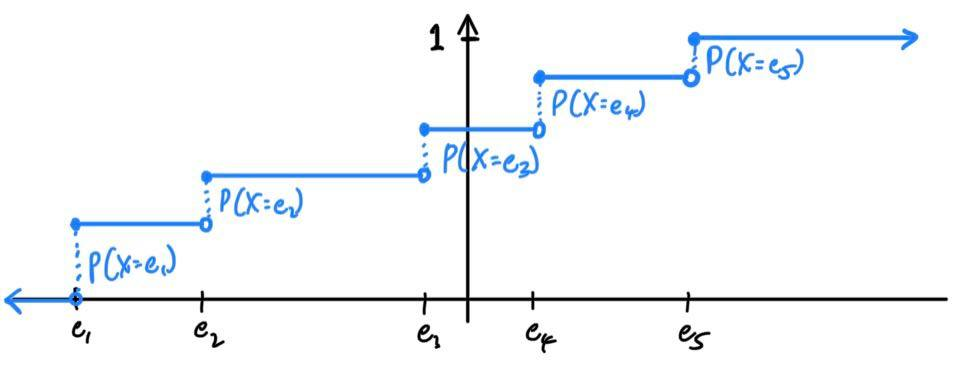
\includegraphics[scale=0.25]{img/Discrete_CDF.jpg}
    \end{center}
    If $E$ was countable, then it would have countably infinite discontinuities. Now we'll give some examples of discrete random variables, and in here we'll completely ignore the sample space $\Omega$, since once we have a random variable $X$, we can just work in $(\mathbb{R}, \mathcal{R}, \mathbb{P}_X)$. Remember that we will write $P(X = x)$ as shorthand for $\mathbb{P}_X (\{x\})$. 

    \begin{definition}[Indicator/Bernoulli Random Variable]
      Given $(\Omega, \mathcal{F}, \mathbb{P})$, let $A \in \mathcal{F}$ be an event. A useful random variable is the \textbf{indicator random variable} $1_A: \Omega \longrightarrow \mathbb{R}$ defined  
      \begin{equation}
        1_A (\omega) = \begin{cases} 1 & \text{ if } \omega \in A \\ 0 & \text{ if } \omega \not\in A \end{cases}
      \end{equation}
      This is a random variable since the preimages of $\emptyset, \{0\}. \{1\}, \{0, 1\}$ are $\emptyset, A^c, A, \Omega$, which are all $\mathcal{F}$-measurable. Since the probability measure of $A$ is $\mathbb{P}(A) = p$, then $\mathbb{P}(A^c) = 1 - \mathbb{P}(A) = 1 - p$, and so we get the PMF 
      \begin{equation}
        p_{1_A} (x) = \begin{cases} 1 - p & \text{ if } x = 0 \\ p & \text{ if } x = 1 \end{cases}
      \end{equation}
      The CDF of this function will look like a step function 
      \begin{equation}
        F_{1_A} (x) = \begin{cases} 0 & \text{ if } x < 0  \\ P(A^c) & \text{ if } 0 \leq x < 1 \\ 1 & \text{ if } 1 \leq x \end{cases}
      \end{equation}
    \end{definition}

    \begin{example}[Uniform Random Variable]
      Given a finite set $E = \{e_i\}_{i=1}^n \subset \mathbb{R}$, we define the PMF as 
      \begin{equation}
        p_X (e_i) = \mathbb{P}(X = e_i) = \frac{1}{n} \; \forall i = 1, 2, \ldots n
      \end{equation}
      which induces the probability measure $\mathbb{P}_X (B) = \sum_{x \in E \cap B} p_X (x)$. 
    \end{example}

    The Bernoulli RV leads to the geometric and binomial random variables. 

    \begin{example}[Geometric Random Variable]
      Given $E = \mathbb{N}$, we can define the PMF associated with random variable $X \sim \mathrm{Geometric}(p)$ as 
      \begin{equation}
        p_X (k) =\mathbb{P}(X = k) = (1 - p)^{k-1} p \text{ for } k \in \mathbb{N}, \; p \in [0, 1]
      \end{equation}
      which induces the probability measure $\mathbb{P}_X (B) = \sum_{x \in E \cap B} p_X (x)$. We can interpret this as the number of times you have to (independently) toss a $p$-coin (probability of heads is $p$) until you get a heads. 
    \end{example}

    \begin{example}[Binomial Random Variable]
      We let $E = \mathbb{N}_0$ and define the PMF associated with random variable $X \sim \mathrm{Binomial}(n, p)$ as 
      \begin{equation}
        p_X (k) = \mathbb{P}(X = k) = \binom{n}{k} p^k (1 - p)^{n - k} \text{ for } k \in E, p \in [0, 1]
      \end{equation}
      We can interpret this as the number of heads occurring in a sequence of $n$ independent tosses of a $p$-coin. 
    \end{example}

    \begin{example}[Poisson Random Variable]
      We let $E = \mathbb{N}_0$ and define the PMF of $X \sim \mathrm{Poisson}(\lambda)$ as 
      \begin{equation}
        p_X (k) = \frac{e^{-\lambda} \lambda^k}{k!} \text{ for } k \in E, \; \lambda > 0
      \end{equation}
    \end{example}

    \begin{definition}[Negative Binomial Distribution]
      The negative binomial distribution, denoted NB$(r, p)$ is defined as
      \begin{equation}
        \mathbb{P}(X = x) \equiv \binom{k+r-1}{k} \, (1-p)^r \, p^k
      \end{equation}
      It can be interpreted as the distribution that models the number of successes in a sequence of iid Bernoulli-$p$ trials before a specified number $r$ failures occurs. 
    \end{definition}

    A slight generalization of a discrete random variable is a simple random variable. Recall that the indicator random variable is a function $1_A: \Omega \rightarrow \mathbb{R}$ defined 
    \begin{equation}
      1_A (\omega) \coloneqq \begin{cases} 1 & \text{ if } \omega \in A \\
      0 & \text{ if else } \end{cases}
    \end{equation}
    As simple random variable generalizes this into multiple sets that form a partition of $\Omega$. It is analogous to a simple function, introduced in measure theory. 

    \begin{definition}[Simple Random Variable]
      Let $\{A_i\}_i$ form a partition of probability space $\Omega$. A \textbf{simple random variable} $X$ is a random variable of the form 
      \begin{equation}
        X (\omega) = \sum_{i} a_i 1_{A_i} (\omega)
      \end{equation}
      that assigns value $a_i$ if the input $\omega \in A_i$. 
    \end{definition}

    Now, let's move on to continuous random variables. 

    \begin{definition}[Absolutely Continuous Measures]
      Let $\mu, \nu$ be measures defined on $(\Omega, \mathcal{F})$. We say that $\nu$ is \textbf{absolutely continuous} w.r.t. $\mu$ if for every $N \in \mathcal{F}$ s.t. $\mu(N) = 0$, we have $\nu(N) = 0$. 
    \end{definition}

    \begin{definition}[Continuous Random Variable]
      A random variable $X$ is \textbf{continuous} if its induced measure $\mathbb{P}_X: (\mathbb{R}, \mathcal{R}) \rightarrow [0, 1]$ is absolutely continuous w.r.t. the Lebesgue measure $\lambda: (\mathbb{R}, \mathcal{R}) \rightarrow \mathbb{R}$, i.e. if for every Borel set $N$ of Lebesgue measure $0$, we have $\mathbb{P}_X (N) = 0$ also. 
    \end{definition}

    A common misconception is that a random variable $X$ is continuous if the induced measure on every singleton set in $\mathcal{B}(R)$ is $0$, i.e. $\mathbb{P}_X (\{x\}) = 0$ for all $x \in \mathbb{R}$. The definition above implies this since the Lebesgue measure of every singleton set is $0$. 

    We introduce a theorem that is useful to know, but we won't prove it. 

    \begin{theorem}[Radon-Nikodym Theorem (Special Case)]
      Let $X$ be a continuous random variable. Then, there exists a nonnegative measurable function $f_X : \mathbb{R} \longrightarrow [0, \infty)$ s.t. for any $B \in \mathcal{R}$, we have 
      \begin{equation}
        \mathbb{P}_X (B) = \int_B f_X \, d\lambda
      \end{equation}
      where the above is the Lebesgue integral. Note that we must define using the Lebesgue integral because Riemann integral is not compatible with any Borel set. $f_X$ is called the \textbf{probability density function}, aka \textbf{PDF}. Furthermore, we can get $f_X$ from $\mathbb{P}_X$ by taking the \textbf{Radon-Nikodym derivative} (which we will not define now)
      \begin{equation}
        f_X = \frac{d \mathbb{P}_X}{d \lambda}
      \end{equation}
      which basically says that if we have a set of very small Lebesgue measure $d \lambda$ tending to $0$, then its probability measure $\mathbb{P}_X$ will also be very small, and the infinitesimal ratio of these two measures on an arbitrarily small set is $f_X$. Also, note that the integral does not change if the value of $f$ changes on sets of Lebesgue measure $0$, and so there is no unique PDF describing $\mathbb{P}_X$. It is unique up to sets of Lebesgue measure $0$, so when we refer to such a PDF $f_X$, we are really talking about an equivalence class of functions. 
    \end{theorem}

    This theorem guarantees the existence of some $f_X$ that completely describes the probability law $P_X$! Take a special case of when $B = (-\infty, x])$, and we can define the CDF as 
    \begin{equation}
      F_X (x) = P_X ((-\infty, x]) = \int_{(-\infty, x]} f_X \, d\lambda
    \end{equation}
    If the set of integration is an interval (and the function is continuous a.e.), then the Lebesgue integral and Riemann integral coincides, and we get the familiar formula 
    \begin{equation}
      F_X (x) = \int_{-\infty}^x f_X (t)\,dt
    \end{equation}
    and we can differentiate it to get back the PDF $f_X$ (or more accurately, some function that agrees with $f_X$ a.e.). We can show that the CDF of a continuous random variable $X$
    \begin{enumerate}
      \item is absolutely continuous, and 
      \item is differentiable almost everywhere, which means that its PDF will be defined almost everywhere (and we can fill in the undefined points however we want). 
    \end{enumerate}
    Note that the PDF $f_X$ itself has no interpretation as a probability (indeed, we can change its value at a countable number of points to anything we want). It is only when we integrate it over some Borel set that gives us a probability. 

    \begin{example}[Uniform Random Variable]
      Let us define the uniform probability measure $P_X$ on $(\mathbb{R}, \mathcal{R})$ with the CDF 
      \begin{equation}
        F_X = \begin{cases} 0 & \text{ if } x < 0 \\
        x & \text{ if } 0 \leq x \leq 1 \\
        1 & \text{ if } 1 < x \end{cases}
      \end{equation}
      It is differentiable almost everywhere except for at the two points $x = 0$ and $x = 1$. Therefore, the PDF $f_X$ is defined for all real numbers except $x = 0$ and $x = 1$. But it doesn't matter: we can assign any value $f_X$ we want on $0$ and $1$ since it won't affect the integral of it. In this example, we just set 
      \begin{equation}
        f_X = \begin{cases} 1 & \text{ if } 0 \leq x \leq 1 \\
        0 & \text{ if else} \end{cases} 
      \end{equation}
    \end{example}

    \begin{example}[Exponential Random Variable]
      The exponential random variable has the following CDF: 
      \begin{equation}
        F_X (x) = \begin{cases} 1 - e^{-\lambda x} & \text{ if } x \geq 0 \\ 0 & \text{ if } x < 0 \end{cases} \text{ for } \lambda > 0
      \end{equation}
      which is differentiable everywhere except at $x = 0$. Differentiating it (and assigning a convenient value at $x = 0$ $f(0) = \lambda$) gives the PDF 
      \begin{equation}
        f_X (x) = \begin{cases} \lambda e^{-\lambda x} & \text{ if } x \geq 0 \\ 0 & \text{ if else} \end{cases}
      \end{equation}
    \end{example}

    \begin{example}[Gaussian Random Variable]
      The PDF is easier to specify for the Gaussian, so we define the Gaussian RV as having PDF 
      \begin{equation}
        f_X (x) = \frac{1}{\sigma \sqrt{2 \pi}} \exp \bigg( -\frac{(x - \mu)^2}{2 \sigma^2} \bigg) \text{ for } \mu \in \mathbb{R}, \sigma > 0
      \end{equation}
      Note that this PDF decreases very quickly as we get further from $\mu$. The CDF cannot be written in closed form, and we call the CDF of the standard Gaussian the \textbf{error function}: 
      \begin{equation}
        \mathrm{Erf}(x) = F_X (x) = \int_{-\infty}^x \frac{1}{\sqrt{2 \pi}} e^{- t^2 / 2} \, dt
      \end{equation}
    \end{example}

    \begin{example}[Cauchy Random Variable (Standardized)]
      The Cauchy random variable gives the PDF 
      \begin{equation}
        f_X (x) = \frac{1}{\pi} \frac{1}{1 + x^2} \text{ for } x \in \mathbb{R}
      \end{equation}
      Integrating this gives the inverse tangent, which after scaling it down by $\pi$ satisfies the conditions of the CDF. Note that the Cauchy distribution falls off much more slowly around the mean (at a rate of $\frac{1}{1 + x^2}$, like a power law) than the Gaussian (which is even \textit{faster} than an exponential, it is at the rate of $e^{-x^2}$). If such a PDF falls off at a slow rate, like a power law, then this is called a \textit{heavy-tailed random variable}. 
    \end{example}

    \begin{example}[Gamma Random Variable]
      The PDF associated with random variable $X \sim \mathrm{Gamma}(n, \lambda)$ is defined 
      \begin{equation}
        f_X(x) = \frac{\lambda^n x^{n-1}}{\Gamma(n)} e^{-\lambda x} \text{ for } x \geq 0
      \end{equation}
      where $\Gamma$ is the gamma function, which is an extension of the factorial function to the domain of complex numbers. 
      \begin{equation}
        \Gamma(x) \coloneqq \int_{0}^\infty z^{x-1} e^{-z}\, dz, \;\;\;\;\; \text{Re}(x) > 0
      \end{equation}
    \end{example}

    \begin{example}[Beta Random Variable]
      The PDF associated with random variable $X \sim \mathrm{Beta}(\alpha, \beta)$, for positive reals $\alpha, \beta$, is defined 
      \begin{equation}
        f_X (x) \equiv \frac{x^{\alpha-1} \,(1-x)^{\beta-1}}{B(\alpha, \beta)}, \text{ where } B(\alpha, \beta) \equiv \frac{\Gamma(\alpha) \Gamma(\beta)}{\Gamma(\alpha + \beta)}
      \end{equation}
      and $\Gamma$ is the Gamma function. 
    \end{example}

    \begin{example}[Uniform RV defined on Cantor Set]
      The cantor set $C \subset [0, 1]$ is defined by removing $(1/3, 2/3)$ from $[0, 1]$ and then removing the middle third from each interval that remains. We define the distribution on this set by defining its CDF: We set 
      \begin{enumerate}
        \item $F(x) = 0$ for $x \leq 0$ and $F(x) = 1$ for $x \geq 1$. 
        \item $F(x) = 1/2$ for $x \in [1/3, 2/3]$, 
        \item $F(x) = 1/4$ for $x \in [1/9, 2/9]$ and $F(x) = 3/4$ for $x \in [7/9, 8/9]$, ... 
      \end{enumerate}
      and extend $F$ to all of $[0 ,1]$ using monotonicity. 
    \end{example} 

    \begin{example}[Dense Discontinuities]
      Let $q_1, q_2, \ldots$ be an enumeration of the rationals. Let $\alpha_i > 0$ have $\sum_{i=1}^\infty \alpha_i = 1$, and let 
      \begin{equation}
        F(x) = \sum_{i=1}^\infty \alpha_i 1_{[q_i, \infty)} (x)
      \end{equation}
      where $1_{[q_i, \infty)} (x) = 1$ if $x \in [q_i, \infty)$ and $0$ if otherwise. 
    \end{example}

    To summarize, once we have a random variable $X: \Omega \rightarrow \mathbb{R}$, we can throw away the sample space and work in $(\mathbb{R}, \mathcal{R}, \mathbb{P}_X)$ with the induced measure $\mathbb{P}_X$, which is known as the \textbf{probability distribution} of $X$.  
    \begin{enumerate}
      \item If $X$ is discrete, then let there be some at most countable set $E = \{e_i\}$ where $P(E) = 1$. it turns out that $\mathbb{P}_X$ can be completely defined by a probability mass function $p_X : \mathbb{R} \rightarrow \mathbb{R}$ defined 
      \begin{equation}
        p_X (x) = \mathbb{P}_X (\{x\}).
      \end{equation}
      Given that we have this PMF , we can define $\mathbb{P}_X$ as such: Given any Borel $B \in \mathcal{R}$, 
      \begin{equation}
        \mathbb{P}_X (B) = \sum_{x \in E \cap B} p_X (x)
      \end{equation}
      \item If $X$ is continuous, then the Radon-Nikodym Theorem asserts the existence of a nonnegative probability density function $f_X$ that completely describes the probability law $\mathbb{P}_X$. Given that we have this PDF, we can then define $\mathbb{P}_X$ as such: Given any Borel $B \in \mathcal{R}$, 
      \begin{equation}
        \mathbb{P}_X (B) = \int_B f_X \, d\lambda
      \end{equation}
    \end{enumerate}

  \subsubsection{Space of Measurable Functions}

    Now it turns out that the space of $\mathcal{F}$-measurable functions $X: \Omega \rightarrow \mathbb{R}$ forms a function space, which means that the set of all random variables on $\Omega$ forms a vector space. We formally show it here. 

    \begin{lemma}
      The set of all $\mathcal{F}$-measurable functions $X: (\Omega, \mathcal{F}) \rightarrow \mathbb{R}$ forms a vector space, denoted $L_\mathcal{F} (\Omega; \mathbb{R})$, or $L_\mathcal{F} (\Omega)$ for short. 
    \end{lemma}
    \begin{proof}

    \end{proof}

    Naturally, we can put the $L^p$-norm on this space, defined 
    \begin{equation}
      ||X||_p \coloneqq \bigg( \int_\Omega |X|^p \, d\mathbb{P} \bigg)^{1/p}
    \end{equation}
    Moreover, if $p = 2$, then we can put an inner product defined 
    \begin{equation}
      \langle X, Y \rangle = \bigg( \int_\Omega X Y \,d \mathbb{P} \bigg)^{1/2}
    \end{equation}

    \begin{definition}
      The Banach space of $\mathcal{F}$-measurable functions is denoted $L_\mathcal{F}^p (\Omega)$, and the Hilbert space is denoted $L_\mathcal{F}^2 (\Omega)$. 
    \end{definition}

    This means that if we have some probability space $(\Omega, \mathcal{F}, \mathbb{P})$ and  sub-$\sigma$-algebra $\mathcal{G} \subset \mathcal{F}$, then any $\mathcal{G}$-measurable function is also $\mathcal{F}$-measurable, since if the preimage of every $B \in \mathcal{R}$ is in $\mathcal{G}$, then it $B \in \mathcal{F}$. This immediately results in the following. 

    \begin{theorem}
      If $\mathcal{G}$ is a sub-$\sigma$-algebra of $\mathcal{F}$, then $L_\mathcal{G} (\Omega)$ is a subspace of $L_\mathcal{F} (\Omega)$. 
    \end{theorem}

    This means that as we get coarser and coarser random variables, the space in which these random variables live in get smaller and smaller, until we get to the constant random variables, which form a $1$-dimensional line in $L_\mathcal{F} (\Omega)$. The origin is simply the constant $0$ random variable. 

\subsection{Independence}

  \begin{definition}[Independence of $2$ Events]
    Given probability space $(\Omega, \mathcal{F}, \mathbb{\mathbb{P}})$, events $A, B \in \mathcal{F}$ are said to be \textbf{independent under $\mathbf{\mathbb{P}}$} if 
    \begin{equation}
      \mathbb{P}(A \cap B) = \mathbb{P}(A) \, \mathbb{P}(B)
    \end{equation}
    This leads to the immediate property that if $\mathbb{P}(B) > 0$, with $A, B$ independent, then 
    \begin{equation}
      \mathbb{P}(A \mid B) = \mathbb{P}(A)
    \end{equation}
  \end{definition}

  Note that $A$ and $B$ may be independent under one measure, but not under another measure. The property that $\mathbb{P}(A \mid B) = \mathbb{P}(A)$ is \textit{not} the definition of independence, since it has the more restricting property that $\mathbb{P}(B) > 0$, so only refer to the definition that $\mathbb{P}(A \cap B) = \mathbb{P}(A) \, \mathbb{P}(B)$. This is the true definition of independent events that we should rely on, not the one that says that $A$ and $B$ are independent if "one does not affect the other." This old definition is misleading and false. For example, take the probability space $[0, 1]$, with Borel $\sigma$-algebra, and Lebesgue measure $\mathbb{P} = \lambda$, and let $A = \mathbb{Q}$ and $B = \mathbb{R} \setminus \mathbb{Q}$. Then, contradictory to our old definition, $A$ and $B$ are independent since $\mathbb{P}(A \cap B) = \mathbb{P}(A) \, \mathbb{P}(B) = 0$! By the definition, an event $A$ is independent of itself if $\mathbb{P}(A) = 0$ or $1$ (e.g. $A$ is rationals, irrationals, cantor set, $\emptyset$, $\Omega$, etc.). 

  \begin{definition}[Independence of $n$ Events]
    Given probability space $(\Omega, \mathcal{F}, \mathbb{P})$, 
    \begin{enumerate}
      \item Let us have a finite collection of events $A_1, A_2, \ldots, A_n \in \mathcal{F}$. They are \textbf{independent} if for all nonempty $I_0 \subset \{1, 2, \ldots n\}$, 
      \begin{equation}
        \mathbb{P} \bigg( \bigcap_{i \in I_0} A_i \bigg) = \prod_{i \in I_0} \mathbb{P}(A_i)
      \end{equation}
      Note that it is not enough to just prove that 
      \begin{equation}
        \mathbb{P}(A_1 \cap \ldots \cap A_n) = \prod_{i=1}^n \mathbb{P}(A_i)
      \end{equation}
      We must verify this for all $2^n$ possible choices (to be precise, we don't need to prove for $I_0 = \emptyset$ and $I_0 = \{A_i\}$), so for $2^n - n - 1$ choices. 
      
      \item Let $\{A_i\}_{i \in I}$ be a collection of events indexed by a possibly uncountable $I$. They are independent if for all nonempty and finite $I_0 \subset I$, we have 
      \begin{equation}
        \mathbb{P} \bigg( \bigcap_{i \in I_0} A_i \bigg) = \prod_{i \in I_0} \mathbb{P}(A_i)
      \end{equation}
    \end{enumerate}
  \end{definition}

  Now when we are trying to compare two $\sigma$-algebras, the measure defined for one may not even be defined on the other. To ensure that a measure is defined on both, it makes sense to take its $\sigma$-algebra and construct two sub-$\sigma$-algebras, which $\mu$ is guaranteed to be defined on. 

  \begin{definition}[Independence of $\sigma$-Algebras]
    Let us have probability space $(\Omega, \mathcal{F}, \mathbb{P})$. 
    \begin{enumerate}
      \item Let $\mathcal{F}_1, \mathcal{F}_2$ be two sub-$\sigma$-algebras of $\mathcal{F}$. $\mathcal{F}_1$ and $\mathcal{F}_2$ are independent if for any $A_1 \in \mathcal{F}_1, A_2 \in \mathcal{F}_2$, $A_1$ and $A_2$ are independent. 
      \item Let $\{ \mathcal{F}_i\}_{i \in I}$ be an arbitrary collection of sub-$\sigma$-algebras of $\mathcal{F}$, indexed by possibly uncountable $I$. Then, they are independent if for any choices of $A_i \in \mathcal{F}_i$ for $i \in I$, $\{A_i\}_{i \in I}$ are independent events. 
    \end{enumerate}
  \end{definition}

  \begin{definition}[Independent Random Variables]
    Two random variables $X, Y$ are \textbf{independent} if $\sigma(X)$ and $\sigma(Y)$ are independent $\sigma$-algebras. That is, for any Borel sets $B_1, B_2 \in \mathcal{R}$, the events $X^{-1}(B_1)$ and $Y^{-1}(B_2)$ are independent: 
    \begin{equation}
      \mathbb{P}\big[ X^{-1}(B_1) \cap Y^{-1}(B_2) \big] = \mathbb{P}(X^{-1}(B_1)) \, \mathbb{P}(Y^{-1}(B_2))
    \end{equation}
    or by abusing notation, 
    \begin{equation}
      \mathbb{P}(X \in B_1, Y \in B_2) = \mathbb{P}(X \in B_1) \, \mathbb{P}(Y \in B_2)
    \end{equation}
  \end{definition}

  If $X, Y$ are independent, then we can say something about the CDFs 
  \begin{equation}
    F_{X, Y} (x, y) = F_X (x) \, F_Y (y)
  \end{equation}
  In fact, we can say something stronger. 

  \begin{theorem}
    $X$ and $Y$ are independent RVs if and only if 
    \begin{equation}
      F_{X, Y} (x, y) = F_X (x) \, F_Y (y)
    \end{equation}
  \end{theorem}

  Moving onto multiple variables, we can define that $X_1, X_2, \ldots, X_n$ are independent RVs if $\sigma(X_1), \ldots, \sigma(X_n)$ are independent $\sigma$-algebras. 

\subsection{Functions of Random Variables}

  In many applications, it happens that we are interested not in the value of the random variable $X$, but a function of it. That is, given a probability space $(\Omega, \mathcal{F}, \mathbb{P})$, let us have a random variable $X: \Omega \rightarrow \mathbb{R}$. We can then define another function $f: \mathbb{R} \rightarrow \mathbb{R}$ and consider the potential random variable $f \circ X : \Omega \rightarrow \mathbb{R}$. We say potential because we don't know yet whether $f \circ X$ is measurable (i.e. the preimage of every Borel set in $\mathbb{R}$ is in $\mathcal{F}$). This condition suffices if $f$ itself is a measurable function, i.e. for every Borel set $B \in \mathcal{R}$, its preimage $f^{-1} (B)$ is Borel in $\mathbb{R}$, and by measurablility of $X$, its preimage under $X$ is $\mathcal{F}$-measurable, making $f \circ X$ a viable random variable. With this new random variable $f \circ X$, we would now like to answer the question: What is the probability law $\mathbb{P}_{f \circ X}$ of $\mathbb{R}$? 

  This also works for joint random variables, which we will learn later. Given a joint random variable $(X_1, X_2, \ldots X_n): \Omega \rightarrow \mathbb{R}^n$, we can define a measurable function $f: \mathbb{R}^n \longrightarrow \mathbb{R}$ and define the scalar random variable $f \circ (X_1, \ldots X_n)$ on $\Omega$. But again, we want to find what the CDF of this composition. 

  \subsubsection{Maximum/Minimum of Random Variables}

    Let $X_1, X_2, \ldots, X_n$ be random variables of $(\Omega, \mathcal{F}, \mathbb{P})$ with joint CDF $F_{X_1 \ldots X_n} (x_1, \ldots, x_n)$. Let $Y_n = \min (X_1, \ldots, X_n)$ and $Z_n = \max(X_1, \ldots, X_n)$. Note that $Y_n$ and $Z_n$ are also functions of $\Omega$ to $\mathbb{R}$. To prove that they are random variables, we just have to prove that $\min$ and $\max$ are measurable functions from $\mathbb{R}^n$ to $\mathbb{R}$, which we can do by proving that the preimage of all semi-infinite interval $(-\infty, x]$ are Borel in $\mathbb{R}^n$. 
    \begin{enumerate}
      \item The preimage of $(-\infty, x]$ under $\max$ is just the set of all $n$-vectors whose max is less than $x$, which is just the semi-infinite cuboid $(-\infty, x]^n \subset \mathbb{R}^n$, which is Borel in $\mathbb{R}^n$. 
      \item The preimage of $(-\infty, x]$ under $\min$ is the set of all $n$-vectors whose min is less than $x$, i.e. at least one element must be less than $x$. But this is just the complement of all vectors that have elements all greater than $x$, which is $\mathbb{R}^n \setminus (x, +\infty)^n \subset \mathbb{R}^n$, which is Borel in $\mathbb{R}^n$. 
    \end{enumerate}
    Now we must determine the CDF of $Y_n$ and $Z_n$. 
    \begin{enumerate}
      \item We have 
      \begin{align*}
        F_{Z_n} (z) & = \mathbb{P}(\{ \omega \mid Z_n (\omega) \leq z \}) \\
        & = \mathbb{P}(\{ \omega \mid X_1 (\omega) \leq z, \ldots, X_n (\omega) \leq z\}) \\
        & = F_{X_1 \ldots X_n} (z, \ldots, z)
      \end{align*}
      where the last equality is describes simply the joint CDF of the joint distribution $(X_1, \ldots, X_n)$. If we assume independence of $X_i$'s, it simplifies out to 
      \begin{equation}
        \prod_{i} F_{X_i} (z)
      \end{equation}
      and if iid, then we have $[F_{X} (z) ]^n$, where $X$ is the common distribution. 
      \item For $Y_n$, we work with complements again and have 
      \begin{align*}
        F_{Y_n} (y) & = \mathbb{P}(\{ \omega \mid Y_n (\omega) \leq y \}) \\ 
        & = 1 - \mathbb{P}(\{ \omega \mid Y_n (\omega) > y \}) \\
        & = 1 - \mathbb{P}(\{ \omega \mid X_1 (\omega) > y, \ldots X_n (\omega) > y \}) \\
      \end{align*}
      where $\mathbb{P}(\{ \omega \mid X_1 (\omega) > y, \ldots X_n > y \})$ can be calculated from the joint distribution. If we assume independence of $X_i$, it simplifies out to 
      \begin{equation}
        1 - \prod_{i} \mathbb{P}(\{\omega \mid X_i(\omega) > y \}) = 1 - \prod_{i} \big( 1 - F_{X_i} (y) \big)
      \end{equation}
      and if iid, then we have $1 - [1 - F_{X} (y)]^n$. 
    \end{enumerate}

    \begin{example}[Uniforms]
      Let $X_1, X_2$ be iid distributed as $\mathrm{Uniform}[0, 1]$, and let $Z = \max(X_1, X_2)$ with $Y = \min(X_1, X_2)$, i.e. $Z$ is the greater of the two and $Y$ is the lesser. We would expect the PDF of $Z$ to have more mass towards $1$ and the PDF of $Y$ to have more mass towards $0$. Our common CDF is 
      \begin{equation}
        F_{X} (x) = \begin{cases} 0 & \text{ if } x < 0 \\
        x & \text{ if } 0 \leq x \leq 1 \\
        1 & \text{ if } 1 < x \end{cases}
      \end{equation}
      Let's calculate the CDF of $Z$. 
      \begin{align*}
        F_{Z} (z) & = \mathbb{P}(\{\omega \mid Z(\omega) \leq z\}) \\
        & = \mathbb{P}(\{ \omega \mid X_1 (\omega) \leq z, X_2 (\omega) \leq z\}) \\
        & = F_{X_1, X_2} (z, z) \\
        & = [F_{X} (z)]^2 = \begin{cases} 0 & \text{ if } x < 0 \\
        x^2 & \text{ if } x \in [0, 1] \\
        1 & \text{ if } 1 < x \end{cases}
      \end{align*}
      This CDF is differentiable everywhere except the two points $0$ and $1$, so we can get the PDF to be $f_Z (z) = 2 z$ for $z \in (0, 1)$ and $0$ otherwise. For the values of $f_Z$ at $0$ and $1$, we can fill it in with anything we want (since the measure of these sets are $0$), so we will just defined $f_Z (0) = 0$ and $f_Z(1) = 2$, getting 
      \begin{equation}
        f_Z (z) = \begin{cases} 2 z & \text{ if } z \in [0, 1] \\
        0 & \text{ if else} \end{cases}
      \end{equation}
      Let's calculate the CDF of $Y$. 
      \begin{align*}
        F_{Y} (y) & = \mathbb{P}(\{ \omega \mid Y(\omega) \leq y\}) \\
        & = 1 - \mathbb{P}(\{ \omega \mid Y(\omega) > y\}) \\
        & = 1 - \mathbb{P}(\{\omega \mid X_1 (\omega) > y, X_2 (\omega) > y \}) \\
        & = 1 - \mathbb{P}(\{\omega \mid X_1 (\omega) > y\}) \, \mathbb{P}(\{ X_2 (\omega) > y \}) \\ 
        & = 1 - [1 - F_X (y)]^2 = \begin{cases} 0 & \text{ if } y < 0 \\
        1 - (1 - y)^2 & \text{ if } y \in [0, 1] \\
        1 & \text{ if } y > 1 \end{cases} 
      \end{align*}
      and differentiating it (with setting any values of the PDF at the nondifferentiable points $0$ and $1$) gives 
      \begin{equation}
        f_Y (y) = \begin{cases} 2 - 2y & \text{ if } y \in [0, 1] \\
        0 & \text{ if else} \end{cases}
      \end{equation}
    \end{example}

    \begin{example}[Exponentials]
      Let $X_1, X_2, \ldots, X_n$ be independent exponential random variables with parameters $\lambda_1, \ldots, \lambda_n$, respectively (not identical!). Then, for each $X_i$, its CDF is 
      \begin{equation}
        F_{X_i} (x) = 1 - e^{-\lambda_i x} \text{ for } x \geq 0
      \end{equation}
      and let $Y = \min(X_1, \ldots, X_n)$. Then, we have 
      \begin{align*}
        F_Y (y) & = 1 - \prod_{i=1}^n [ 1 - F_{X_i} (y)] \\
        & = 1 - \prod_{i=1}^n e^{-\lambda_i x} \\
        & = 1 - e^{- ( \sum_{i=1}^n \lambda_i ) x}
      \end{align*}
      which is the CDF of an exponential distribution. So, 
      \begin{equation}
        Y \sim \mathrm{Exponential}(\lambda_1 + \ldots + \lambda_n)
      \end{equation}
      This is nice, since the minimum of a bunch of exponentials is an exponential. However, this is not the case for the maximum. 
    \end{example}

    This has nice practical applications. For example, recall the memoryless property of the exponential, which nicely models radioactive decay. If we have $n$ elements each decaying at some $\mathrm{Exponential}(\lambda_i)$ rate, then we can model the time at which the first alpha particle will emit amongst all $n$ elements will also be an exponential. These processes where the inter-emission times are exponentials are called Poisson process, which we will discuss later. 

    \begin{definition}[Order Statistic]
      Let $X_1, X_2, ..., X_n$ be a finite collection of independent, identically distributed random variables. Suppose that they are continuously distributed with density $f$ and CDF $F$. Define the random variable $X_{(k)}$ to be the $k$th ranked value, called the \textbf{$k$th order statistic}. This means that 
      \begin{equation}
        X_{(1)} = \min\{X_1, X_2, ..., X_n\}, \;\; X_{(n)} = \max\{X_1, X_2, ..., X_n\}
      \end{equation}
      and in general, for any $k \in \{1, 2, ..., n\}$, 
      \begin{equation}
        X_{(k)} = X_j \text{ if } \sum_{l=1}^n \mathbb{I}_{X_l < X_j} = k - 1
      \end{equation}
      which means that exactly $k-1$ of the values of $X_l$ are less than $X_j$. Since $F$ is continuous, 
      \begin{equation}
        X_{(1)} < X_{(2)} < ... < X_{(n)}
      \end{equation}
      holds with probability $1$. This leads us to define the random variable $X_{(k)}$ representing the $k$th order statistic.
      \begin{equation}
        f_{(k)} (y) = \begin{cases} 
        n \, \binom{n-1}{k-1} y^{k-1} (1-y)^{n-k} & y \in (0, 1) \\
        0 & y \not\in (0,1)
        \end{cases}
      \end{equation}
      That is, $X_{(k)}$ has the Beta$(k, n-k_1)$ distribution. 
    \end{definition}

  \subsubsection{Convolutions and Sums of Random Variables}

    Now given two random variables $X, Y: \Omega \rightarrow \mathbb{R}$ that each push their own probability laws $\mathbb{P}_X, \mathbb{P}_Y$ onto $\mathbb{R}$, their sum $Z = X + Y$ is also a random variable that pushes its own probability law $\mathbb{P}_Z$. We must actually prove that $Z$ is a random variable, which we can do by proving that the preimage of every $(-\infty, x]$ is $\mathcal{F}$-measurable. Equivalently (by complementation), we must prove that the preimage of every $(x, +\infty)$ (that is, all sets of form $\{ \omega \mid Z(\omega) > z\}$) is $\mathcal{F}$-measurable. Now we can write $z$ as the sum of two numbers $z = q + (z - q)$, where $q \in \mathbb{R}$, and say that 
    \begin{equation}
      \{ \omega \mid Z(\omega) > z\} = \bigcup_{q \in \mathbb{R}} \{ \omega \mid X (\omega) > q , \; Y(\omega) > z - q\}
    \end{equation}
    But using the fact that $\mathbb{Q}$ is dense in $\mathbb{R}$, we can turn this from an uncountable union to a countable union and say 
    \begin{align}
      \{ \omega \mid Z(\omega) > z\} & = \bigcup_{q \in \mathbb{Q}} \{ \omega \mid X (\omega) > q , \; Y(\omega) > z - q\} \\
      & = \bigcup_{q \in \mathbb{Q}} \big( \{\omega \mid X(\omega) > q\} \cap \{ \omega \mid Y(\omega) > z - q\} \big) 
    \end{align}
    and since I have a countable union of (an intersection of) these $\mathcal{F}$-measurable sets, $\{ \omega \mid Z(\omega) > z\}$ is $\mathcal{F}$-measurable, and we are done. This equation above even gives us a hint of how to compute the CDF of $Z$. 

    \begin{theorem}
      Given random variables $X_1, X_2, \ldots, X_n$ of probability space $(\Omega, \mathcal{F}, \mathbb{P})$, 
      \begin{enumerate}
        \item $X_1 + \ldots + X_n$ is a random variable.
        \item $X_1 \cdot \ldots \cdot X_n$ is a random variable. 
      \end{enumerate}
    \end{theorem}

    For simplicity, we will only consider jointly discrete or jointly continuous random variables. The probability law $\mathbb{P}_Z$ can be confusing to define, since given some Borel set $B \in \mathcal{R}$, we must now look at the preimage under the \textit{sum} $X + Y$. A simpler way to approach this is to consider the joint distribution $X, Y$ and look at its distribution, which we call the \textbf{convolution} of $X$ and $Y$. This is especially simple to consider for discrete random variables. 

    \begin{definition}[Sums of Discrete Random Variables]
      Take two discrete random variables $X, Y$ with their joint PMF $p_{X, Y} (x, y)$ and their sum $Z = X + Y$. We can see that the PMF of $Z$ is 
      \begin{equation}
        p_Z (z) = \sum_{(x, y) \,:\, x + y = z} p_{X, Y} (x, y) = \sum_{x \in \mathcal{X}} p_{X, Y} (x, z - x)
      \end{equation}
      which by abuse of notation, we denote
      \begin{equation}
        \mathbb{P}(Z = z) = \sum_{x \in \mathcal{X}} \mathbb{P}(X = x, Y = z - x)
      \end{equation}
      The CDF is very simple, since we just have to sum over all $(x, y)$ such that their sum is less than $z$: 
      \begin{equation}
        F_Z (z) = \sum_{(x, y) \,:\, x + y \leq z} p_{X, Y} (x, y)
      \end{equation}
      which by abuse of notation, we write 
      \begin{equation}
        \mathbb{P}(Z \leq z) = \sum_{(x, y) \,:\, x + y \leq z} \mathbb{P}(X = x, Y = y)
      \end{equation}
      If $X$ and $Y$ are independent, then their joint distribution is the product of their singular distributions, and so we have 
      \begin{equation}
        p_Z (z) = \sum_x p_X (x) \, p_Y (z - x) \coloneqq p_X \ast p_Y
      \end{equation}
      where $p_Z = p_X \ast p_Y$ is called the convolution of $p_X$ and $p_Y$. By abuse of notation, 
      \begin{equation}
        \mathbb{P}(Z = z) = \sum_{x \in \mathcal{X}} \mathbb{P}(X = x) \, \mathbb{P}(Y = z - x)
      \end{equation}
    \end{definition}

    \begin{example}[Sums of Poisson RVs]
      Let $X_1$ and $X_2$ be independent Poisson random variables with parameters $\lambda_1, \lambda_2 > 0$, and let $Z = X_1 + X_2$. The PMF of each $X_i$ is 
      \begin{equation}
        p_{X_i} (k) = \frac{e^{-\lambda_i} \lambda_i^k}{k!} \text{ for } k \in \mathbb{Z}
      \end{equation}
      and taking the convolution gives the PMF of $Z$: 
      \begin{align*}
        p_Z (z) & = (p_{X_1} \ast p_{X_2}) (z) \\
        & = \sum_{k=-\infty}^{+\infty} \frac{e^{-\lambda_1} \lambda_1^k}{k!} \cdot \frac{e^{-\lambda_2} \lambda_2^{z - k}}{(z - k)!} \\
        & = \sum_{k=0}^{z} \frac{e^{-\lambda_1} \lambda_1^k}{k!} \cdot \frac{e^{-\lambda_2} \lambda_2^{z - k}}{(z - k)!} \\ 
        & = \frac{e^{-(\lambda_1 + \lambda_2)}}{z!} \sum_{k=0}^z \binom{z}{k} \lambda_1^k \lambda_2^{z - k} \\
        & = \frac{e^{-(\lambda_1 + \lambda_2)} (\lambda_1 + \lambda_2)^z}{z!} 
      \end{align*}
      for $z \in \mathbb{N}_0$, which is the PMF of another Poisson. So, $Z \sim \mathrm{Poisson}(\lambda_1 + \lambda_2)$. 
    \end{example}

    This has a nice visualization, since the joint distribution of $X$ and $Y$ over $\mathbb{R}^2$ is being "summed up/integrated" over the diagonals of $\mathbb{R}^2$, i.e. the lines where $x + y = z$ for some $z$, sort of like marginalizing over these diagonals. This creates a new "diagonally marginal distribution" $Z$. 

    \begin{definition}[Sums of Continuous Random Variables]
      Take two continuous random variables $X, Y$ with their joint PDF $f_{X, Y} (x, y)$ and their sum $Z = X + Y$. To calculate the CDF, we must basically integrate the joint PDF over the borel set $\{(x, y) \in \mathbb{R}^2 \mid x + y \leq z\}$. 
      \begin{align*}
        \mathbb{P}(Z \leq z) = F_Z (z) & = \int_{(x, y) \,:\, x + y \leq z} f_{X, Y} (x, y) \,dy\,dx \\
        & = \int_{-\infty}^{+\infty} \int_{-\infty}^{z - x} f(x, y) \,dy \,dx
      \end{align*}
      We can see that the PDF of $Z$ is 
      \begin{equation}
        f_{Z} (z) = \int_{\mathbb{R}} f_{X, Y} (x, z - x) \, dx
      \end{equation}
      If $X$ and $Y$ are independent, then 
      \begin{equation}
        f_{Z} (z) = \int_{\mathbb{R}} f_{X} (x) \, f_Y (z - x) \,dx \coloneqq f_X \ast f_Y
      \end{equation}
      where $f_Z = f_X \ast f_Y$ is the convolution of $f_X$ and $f_Y$. 
    \end{definition}

    \begin{definition}[Convolution]
      Given two functions $f, g: \mathbb{R} \longrightarrow \mathbb{R}$, the \textbf{convolution} of $f$ and $g$ is a new function $f \ast g$ defined  
      \begin{equation}
        (f \ast g) (t) \coloneqq \int_\mathbb{R} f(t)\, g(t - \tau) \, d \tau
      \end{equation}
    \end{definition}

    Usually, when we take convolutions, it is not pretty and even for nice distributions like two Gaussians, convolving them is quite complicated. What we can do is transform them (using Laplace, Fourier, etc.) to make calculations easier and more elegant, which we will talk about later.  

    \begin{example}
      Let $X_1$ and $X_2$ be independent exponential with parameters $\lambda_1, \lambda_2$, with individual PDFs $f_{X_i} (x) = \lambda_i e^{-\lambda_i x}$ for $x \geq 0$. Let $Z = X_1 + X_2$. Then, 
      \begin{align*}
        f_Z (z) = (f_{X_1} \ast f_{X_2})(z) & = \int_{-\infty}^\infty \lambda_1 e^{-\lambda_1 x} \, \lambda_2 e^{-\lambda_2 (z -x)} \, dx \\
        & = \int_{0}^z \lambda_1 e^{-\lambda_1 x} \, \lambda_2 e^{-\lambda_2 (z -x)} \, dx \\ 
        & = \lambda_1 \lambda_2 e^{-\lambda_2 z} \int_0^z e^{(\lambda_2 - \lambda_1) x}\,dx \\
        & = \begin{cases} \frac{\lambda_1 \lambda_2}{\lambda_2 - \lambda_1} \big( e^{-\lambda_1 z} - e^{-\lambda-2 z} \big) & \text{ if } \lambda_1 \neq \lambda_2 \\
        \lambda^2 z e^{-\lambda z} & \text{ if } \lambda_1 = \lambda_2 = \lambda \end{cases} 
      \end{align*}
      The distribution for when $\mu_1 = \mu_2$ is called the Erlang distribution, which has many applications, but the other case is an ugly form and not studied very well. 
    \end{example}

    \begin{theorem}[Sums of Discrete Variables]
      Assume that $X$ and $Y$ are independent. 
      \begin{enumerate}
        \item $X \sim$ Binomial$(n, p)$, $Y \sim$ Binomial$(m, p)$ $\implies X + Y \sim$ Binomial$(n + m, p)$. 
        \item $X \sim$ Poisson$(\lambda)$, $Y \sim$ Poisson$(\gamma)$ $\implies X + Y \sim$ Poisson$(\lambda + \gamma)$. 
        \item If $X_1, ..., X_n$ are Geometric$(p)$, then $X_1 + ... + X_n$ is NB$(n, p)$. 
      \end{enumerate}
    \end{theorem}

    \begin{theorem}[Sums of Densities]
      Assume that $X$ and $Y$ are independent. 
      \begin{enumerate}
        \item $X \sim$ Normal$(\mu_1, \sigma_1^2)$, $Y \sim$ Normal$(\mu_2, \sigma_2^2)$ $\implies X + Y \sim$ Normal $(\mu_1 + \mu_2, \sigma_1^2 + \sigma_2^2)$. 
        \item If $X_1, X_2, ..., X_n$ are Exponential$(\lambda)$, then $X_1 + ... + X_n \sim$ Gamma$(n, \lambda)$.
        \item $X \sim$ Gamma$(n, \lambda)$, $Y \sim$ Gamma$(m, \lambda)$ $\implies X + Y \sim$ Gamma$(n + m, \lambda)$. 
        \item $X \sim$ Gamma $(n, \lambda)$, $Y \sim$ Exponential $(\lambda)$ $\implies X + Y \sim$ Gamma$(n+1, \lambda)$. 
      \end{enumerate}
    \end{theorem}

  \subsubsection{Sum of Random Number of Random Variables}

    Now we consider a random variable where the number of terms we are summing is a random variable. Let $\{X_i\}_i$ be a countable sequence of independent random variables with CDF $F_{X_i}$. Let $N$ be a positive integer-valued random variable with PMF $p_N(n) = \mathbb{P}(N = n)$. Assume that $N$ is independent of $X_i$'s. Now, consider the function 
    \begin{equation}
      S_N \coloneqq \sum_{i=1}^N X_i
    \end{equation}
    To interpret this, consider the sample space $\Omega$. We have all $X_i$'s and $N$ defined on the same $\Omega$. Once $\omega \in \Omega$ realizes, the $\{X_i\}$'s will realize as a sequence of numbers, and $N$ will realize as a positive integer. We simply sum them up according to the rule $S_N$, and by this definition, $S_N$ is a real-valued function on $\Omega$. We first have to prove that $S_N$ is a random variable (since we only know that a \textit{fixed} sum of random variables is a random variable), and then we must find the CDF of $S_N$ $\mathbb{P}(S_N \leq x)$. 

    First, note that the realization of $N$ partitions the sample space as 
    \begin{equation}
      \Omega = \bigsqcup_{n = 1}^\infty \{\omega \mid N(\omega) = n\}
    \end{equation}
    Once I have this partition, I can invoke the partition rule and write 
    \begin{align*}
      \mathbb{P}(S_N \leq x) & = \sum_{k=1}^\infty \mathbb{P}(S_N \leq x \mid N = k) \, \mathbb{P}(N = k) \\
      & = \sum_{k=1}^\infty \mathbb{P}(S_k \leq x \mid N = k) \, \mathbb{P}(N = k) & (\text{conditioned on } N = k) \\
      & = \sum_{k=1}^\infty \mathbb{P}(S_k \leq x) \, \mathbb{P}(N = k) & (N \text{ is indep. of } X_i \text{s})
    \end{align*}
    where $\mathbb{P}(N = k)$ is known since we know the PMF of $N$, and the CDFs $\mathbb{P}(S_k \leq x)$ can be computed by computing the deterministic sums and computing their CDF. 

    \begin{example}
      Let $X_i$'s be iid $\mathrm{Exponential}(\lambda)$, and $N \sim \mathrm{Geometric}(p)$. We know that the deterministic sum of iid exponentials gives an Erlang. So, $S_N = \sum_{i=1}^N X_i$, and its CDF is 
      \begin{equation}
        \mathbb{P}(S_N \leq x) = \sum_{k=1}^\infty \mathbb{P}(S_k \leq x) \, \mathbb{P}(N = k)
      \end{equation}
      where $\mathbb{P}(N = k) = (1 - p)^{k - 1} p$. The PDF of the Erlang is 
      \begin{equation}
        p_{S_k} (x) = \frac{\lambda^n x^{n-1}}{(n - 1)!} e^{-\lambda x}
      \end{equation}
      and doing the brute force calculations gives a clean $S_N \sim \mathrm{Exponential}(\lambda p)$. 
    \end{example}

  \subsubsection{General Transformations of Random Variables}

    Now we will look at more general transformations that are not just minimum, maximum, deterministic sums, or random sums. Let us have a probability space $(\Omega, \mathcal{F}, \mathbb{P})$, a random variable $X: \Omega \rightarrow \mathbb{R}$, and a measurable function $f: \mathbb{R} \rightarrow \mathbb{R}$. Now given that we know the CDF (and therefore distribution) of $X$, we want to find the CDF of random variable $Y = f(X) = f \circ X$ (which we have established as a random variable already due to measurability of $f$): $F_Y (y) = \mathbb{P}(Y \leq y)$, which is just $\mathbb{P}_Y ((-\infty, y])$ (where $\mathbb{P}_Y$ is the probability law on $Y$). But rather than trying to take the preimage of the entire composite random variable $Y$ and calculating $\mathbb{P}\big( Y^{-1}((-\infty, y]) \big)$ under the probability on $\mathcal{F}$, let's just take the preimage one step at a time. Note that $f^{-1} \big( (-\infty, y] \big) = \{x \in \mathbb{R} \mid f(x) \leq y\}$. We can then write the CDF of $Y$ in terms of the probability law of $X$: 
    \begin{align*}
      F_Y (y) & = \mathbb{P}_X \big( f^{-1} ((-\infty, y]) \big) \\
      & = \mathbb{P}_X \big( \{x \in \mathbb{R} \mid f(x) \leq y\} \big) \\
      & = \mathbb{P} \big( X^{-1} \circ f^{-1} ((-\infty, y]) \big) 
    \end{align*}
    Depending on how complicated $f$ is, this may be easy or not, but conceptually, this is no problem. But theoretically, this is as far as we can go. Let's move onto some examples. We start with a practical way to generate a Gaussian distribution, which is how most modern software computes. 

    \begin{example}[Box-Muller Transform]
      Given that you have a uniform random number generator in $[0, 1]$, you can generate a normal $N(0, 1)$ by transforming it using the inverse CDF of the normal. This is usually computationally heavy since the inverse CDF of the Gaussian requires expensive operations. An easier way is to use the \textbf{Box-Muller transform}, where you take two uniforms $u_1, u_2$ and transform it as 
      \begin{align*}
          x_1 & = \sqrt{-2 \ln(u_1)} \cos(2 \pi u_2) \\
          x_2 & = \sqrt{-2 \ln(u_1)} \sin(2 \pi u_2)
      \end{align*}
      Once you have $x \sim N(0, 1)$, you can use $\mu + \sigma x \sim N(\mu, \sigma^2)$. You can extend this to a $n$-dimensional normal distribution $\mathbf{x} \sim N(\mathbf{0}, \mathbf{I})$ and transform it to get $\boldsymbol{\mu} + \boldsymbol{\Sigma}^{1/2} \mathbf{x} \sim N(\boldsymbol{\mu}, \boldsymbol{\Sigma})$. 
    \end{example}

    \begin{example}[Chi-Squared Distribution]
      Let $X \sim \mathcal{N}(0, 1)$ and $Y = f(X) = X^2$. Note that $X$ takes values in $(-\infty, +\infty)$ and $Y$ in $[0, +\infty)$. Then, we can write 
      \begin{align*}
        F_Y (y) & = \mathbb{P}(Y \leq y) \\ 
        & = \mathbb{P}_Y ( (-\infty, y]) \\
        & = \mathbb{P}_Y (  [0, y]) & (\text{range of } Y) \\
        & = \mathbb{P}_X ( f^{-1} ([0, y]) ) & (\text{work in prob. law of } X) \\
        & = \mathbb{P}_X ( [-\sqrt{y}, \sqrt{y}] ) \\
        & = \int_{-\sqrt{y}}^{\sqrt{y}} f_X (x) \,dx 
      \end{align*}
      Rewriting this in our abuse of notation notation, we have 
      \begin{align*}
        F_Y (y) & = \mathbb{P}(Y \leq y) \\
        & = \mathbb{P}(X^2 \leq y) \\
        & = \mathbb{P}( -\sqrt{y} \leq X \leq \sqrt{y}) \\
        & = 2 \mathbb{P}(0 \leq X \leq \sqrt{y}) & (\text{Symmetry of Gaussian})\\
        & = \frac{2}{\sqrt{2} \pi} \int_0^{\sqrt{y}} e^{-x^2 / 2} \,dx 
      \end{align*}
      and this is clearly differentiable, since it is written like an integral. Doing so gives the PDF
      \begin{equation}
        f_Y (y) = \frac{1}{\sqrt{2 \pi y}} e^{-y/2} \text{ for } y \geq 0
      \end{equation}
      This describes the PDF of a \textbf{Chi-Squared} distribution. 
    \end{example}

    \begin{example}[Log-Normal Distribution]
      Let $X \sim \mathcal{N}(0, 1)$ and $Y = f(X) = e^X$. Note that the range of $f$ is $(0, +\infty)$. So, 
      \begin{align*}
        F_Y (y) & = \mathbb{P}(Y \leq y) \\
        & = \mathbb{P}_Y ((-\infty, y]) \\
        & = \mathbb{P}_Y ( (0, y]) \\ 
        & = \mathbb{P}_X ( f^{-1} ((0, y]) ) \\
        & = \mathbb{P}_X ( (-\infty, \ln{y}] ) \\
        & = \int_{-\infty}^{\ln{y}} f_X (x)\,dx 
      \end{align*}
      Rewriting this in our abuse of notation notation, we have 
      \begin{align*}
        F_Y (y) & = \mathbb{P}(e^X \leq y) \\
        & = \mathbb{P}(X \leq \ln(y)) \\ 
        & = \int_{-\infty}^{\ln(y)} \frac{1}{\sqrt{2} \pi} e^{-x^2/ 2} \,dx 
      \end{align*}
      We can differentiate this to get 
      \begin{equation}
        f_Y (y) = \frac{1}{y \sqrt{2 \pi}} e^{-\frac{(ln{y})^2}{2}} \text{ for } y \geq 0
      \end{equation}
      This describes the PDF of a \textbf{log-normal} distribution. 
    \end{example}

    We now show a more specific formula under more specific assumptions about the transformation. Suppose $X$ is a \textit{continuous} random variable with density $f_X$ and $g: \mathbb{R} \rightarrow \mathbb{R}$ a monotonic differentiable function. Then, the CDF of the random variable $Y = g(X)$ can be written in the probability law of $X$, which can then by written as an integral by invoking the Radon-Nikodym theorem: 
    \begin{align*}
      \mathbb{P}(Y \leq y) & = \mathbb{P}_X (f^{-1} ((-\infty, y]) \\
      & = \int_{x \,:\, g(x) \leq y} f_X (x) \,dx
    \end{align*}
    Note that we can now talk about the actual inverse $g^{-1}$ since differentaible and monotonic implies invertibility. 
    \begin{enumerate}
      \item Assuming $g$ is monotonically increasing, we can use the change of variables $x = g^{-1} (t)$ and $g(x) = t \implies g^\prime (x) \,dx = dt$ to get the above integral as 
      \begin{equation}
        \int_{-\infty}^{g^{-1} (y)} f_X (x) \,dx = \int_{-\infty}^t \frac{f_X \big( g^{-1} (t) \big)}{g^\prime \big( g^{-1} (t)\big)} \,dt 
      \end{equation}
      but since this is simply the CDF of $Y$, the PDF must equal 
      \begin{equation}
        f_Y (y) = \frac{f_X (g^{-1} (y) )}{g^\prime (g^{-1} (t))}
      \end{equation}
      \item If $g$ is monotonically decreasing, we get 
      \begin{equation}
        f_Y (y) = \frac{f_X (g^{-1} (y) )}{- g^\prime (g^{-1} (t))}
      \end{equation}
    \end{enumerate}
    In general, we can consider both cases by putting an absolute value 
    \begin{equation}
      f_Y (y) = \frac{f_X (g^{-1} (y) )}{|g^\prime (g^{-1} (t))|}
    \end{equation}
    and $g^\prime (g^\prime (y))$ is the Jacobian, the same one that we use when we perform a change of variables in integration. 

    \begin{example}[Log-Normal Revisited]
      Given $X \sim \mathcal{N}(0, 1)$ and $Y = e^X$ (which is monotonically increasing), we can simply plug in the formula to get the PDF: 
      \begin{equation}
        f_Y (y) = \frac{f_X (g^{-1} (y) )}{|g^\prime (g^{-1} (t))|} = \frac{f_X (\ln{y}) }{ | e^{\ln{y}} |} = \frac{1}{\sqrt{2 \pi} y} e^{-(\ln{y})^2 / 2}
      \end{equation}
      for $y > 0$. This domain is important since $\ln{y}$ is only defined for $y > 0$. 
    \end{example}

    \begin{example}
      Given $X \sim \mathcal{N}(0, 1)$ and $Y = f(X) = X^2$, we cannot use the formula since $f$ is not monotonic on the range of $X$, which is $(-\infty, +\infty)$.  
    \end{example}

    \begin{example}
      Given $X \sim \mathrm{Exponential}(\lambda)$ and $Y = f(X) = X^2$, it may seem like the formula is not applicable here, but $f$ \textit{is} monotonic on the range of $X$, which is $[0, + \infty)$. 
    \end{example}

    However, there is much less chance of error by deriving using first principles, so I would recommend using it always rather than these formulas. 

    Let's do the $n$-dimensional version of this. Given random variables $X_1, X_2, \ldots, X_n$ iid random variables with joint density $f_{X_1 \ldots X_n} (x_1, \ldots, x_n)$, we define the transformation $g: \mathbb{R}^n \rightarrow \mathbb{R}^n$ as 
    \begin{equation}
      \begin{bmatrix} Y_1 \\ \vdots \\ Y_N \end{bmatrix} = \begin{bmatrix} g_1 (X_1) \\ \vdots \\ g_n (X_N) \end{bmatrix}
    \end{equation}
    Then, the PDF of $Y$ will be 
    \begin{align*}
      f_{Y_1 \ldots Y_n} (y_1, \ldots, y_n) & = f_{X_1 \ldots X_n} \big( \mathbf{g}^{-1} (\mathbf{y}) \big) \cdot | \mathbf{J}(\mathbf{y})| \\
      & = f_{X_1 \ldots X_n} \big( g_1^{-1}(y_1), \ldots, g_n^{-1} (y_n) \big) \cdot | \mathbf{J}(\mathbf{y})| \\
    \end{align*}
    where 
    \begin{equation}
      \mathbf{J}(y) = \mathrm{det}\begin{pmatrix} 
      \frac{\partial x_1}{\partial y_1} & \ldots & \frac{\partial x_n}{\partial y_1} \\
      \vdots & \ddots & \vdots \\ 
      \frac{\partial x_1}{\partial y_n} & \ldots & \frac{\partial x_n}{\partial y_n} \end{pmatrix}
    \end{equation}


\section{Integration}

  \subsection{Construction of the Riemann Integral}

    We shall first define the integral using the familiar notation of Riemann sums. 

    \begin{definition}[Partitions with Distinguished Points]
      A \textbf{partition} $P$ of a closed interval $[a, b]$, $a < b$, is a finite system of points $x_0, \ldots, x_n$ of the interval such that
      \[a = x_0 < x_1 < x_2 < \ldots < x_n = b\]
      The intervals $[x_{i-1}, x_i]$, $i = 1, 2, \ldots, n$, are called the \textbf{intervals} of the partition $P$. The largest of the lengths of the intervals of the partition $P$, denoted $\lambda(P)$, is called the \textbf{mesh} of the partition. 

      A \textbf{partition with distinguished points} $(P, \xi)$ on the closed interval $[a, b]$ is a partition $P$ of $[a,b]$ along with the set of $n$ points 
      \[\xi_1 \in [x_0, x_1], \xi_2 \in [x_1, x_2], \ldots, \xi_n \in [x_{n-1}, x_n]\]
      The $n$-tuple of $\xi_i$'s is denoted by the single letter $\xi$
      \[\xi = (\xi_1, \xi_2, \ldots, \xi_n)\]
    \end{definition}

    This naturally leads to the following construction. 

    \begin{definition}[Riemann Sums]
      If a function $f$ is defined on a closed interval $[a, b]$ and $(P, \xi)$ is a partition with distinguished points on this closed interval, the sum
      \[\sigma(f; P, \xi) \equiv \sum_{i=1}^n f(\xi_i)\, \Delta x_i, \text{ where } \Delta x_i = x_i - x_{i-1},\]
      is the \textbf{Riemann sum} of the function $f$ corresponding to the partition $(P, \xi)$ with distinguished points on $[a, b]$. 
      \begin{center}
          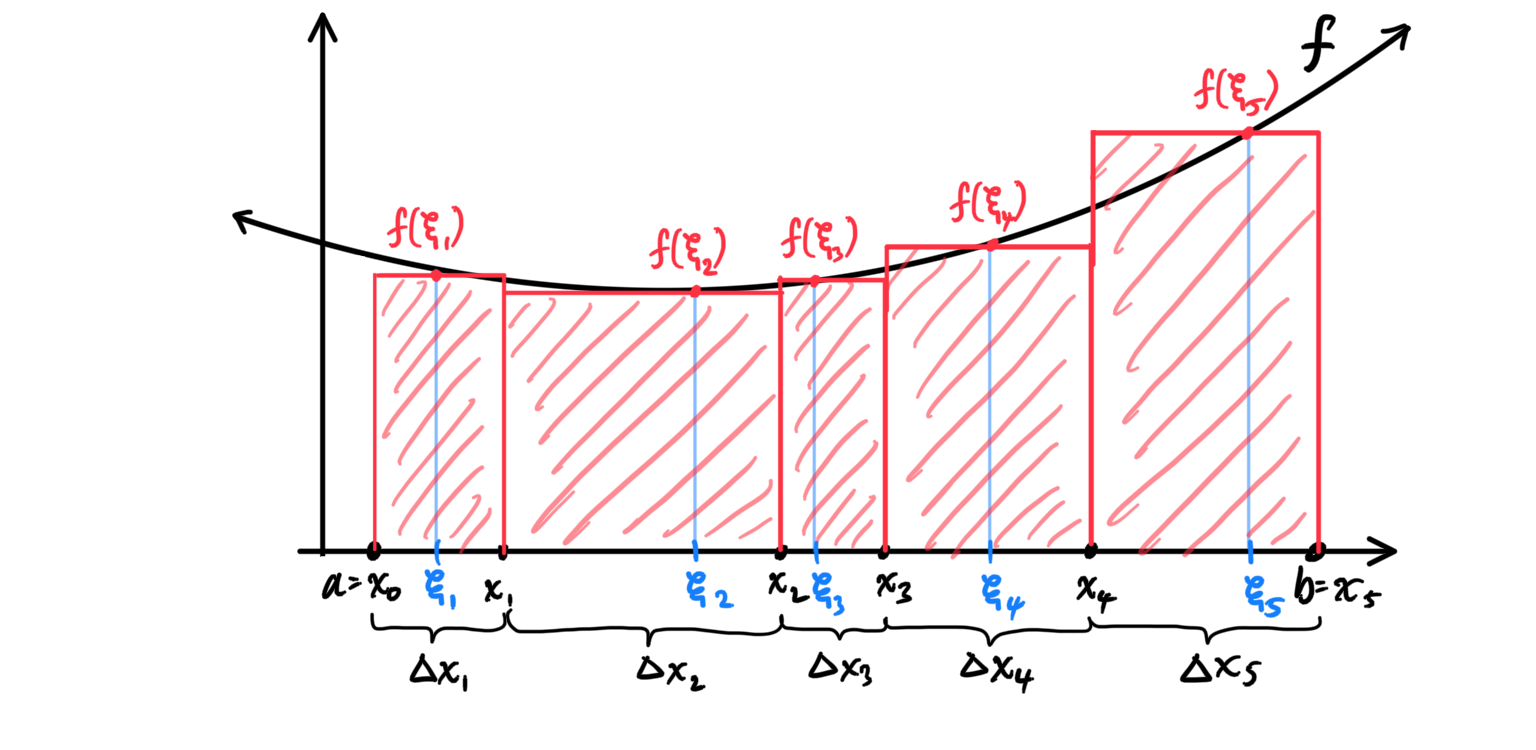
\includegraphics[scale=0.25]{img/Riemann_Sum_with_Partitions_Points.PNG}
      \end{center}
      Thus, when a function $f$ is fixed, the Riemann sum $\sigma (f; P, \xi)$ is a mapping that takes in a partition with distinguished points $p = (P, \xi)$ on the closed interval $[a, b]$ and outputs a number representing the total area of the Riemann sums. That is, for a fixed $f$ and some input $p = (P, \xi)$, we can define the function 
      \[\Phi: \mathcal{P} \longrightarrow \mathbb{R}, \;\;\; \Phi(p) \equiv \sigma(f; p) \equiv \sigma(f; (P, \xi))\]
      that takes in a partition with distinguished points on $[a,b]$ and outputs the corresponding Riemann sum for that fixed $f$. 
    \end{definition}

    \begin{definition}[Riemann Integral]
      The number $\int_a^b f(x)\,dx$ is the \textbf{Riemann integral} of the function $f$ on the closed interval $[a, b]$ if for every $\epsilon>0$ there exists a $\delta>0$ such that
      \[\Bigg| \int_a^b f(x)\,dx - \sum_{i=1}^n f(\xi_i) \Delta x_i \Bigg| < \epsilon\]
      for any partition $(P, \xi)$ with distinguished points on $[a, b]$ whose mesh $\lambda(P)$ is less than $\delta$. We can view this as a limit where $n \rightarrow \infty$, but there is a problem since we can increase the partition within different subsets of $[a,b]$, leading to multiple values of convergence. 
      \begin{center}
          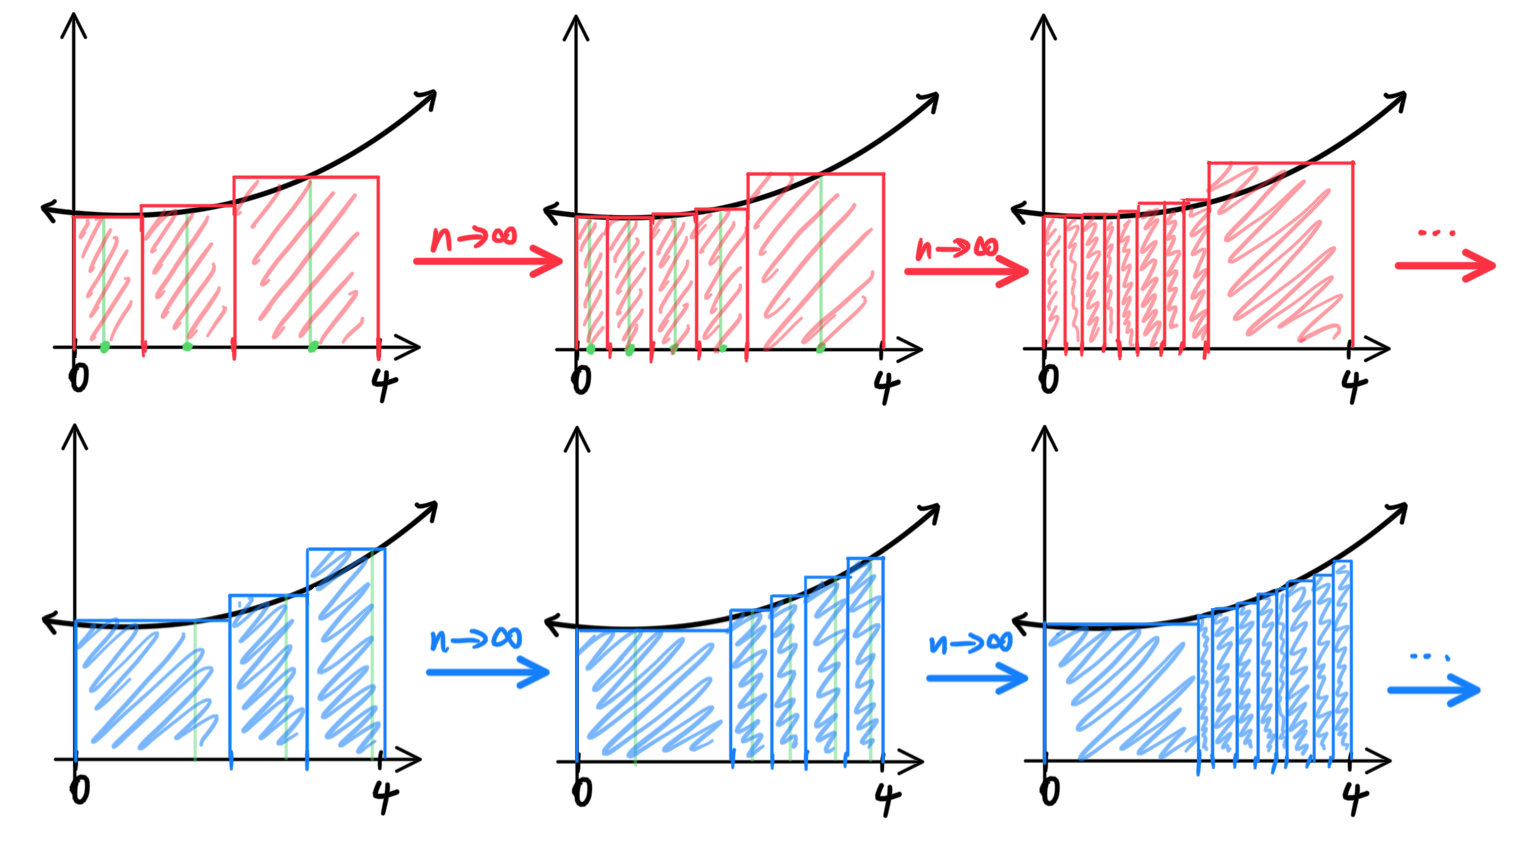
\includegraphics[scale=0.28]{img/Riemann_Integral_Converging_onto_2_Numbers.PNG}
      \end{center}
      Rather, we can set the mesh $\lambda(P)$ to approach $0$, which would take care of the problems. We can visualize this by imagining the lengths of the rectangles converging "uniformly."
      \begin{center}
          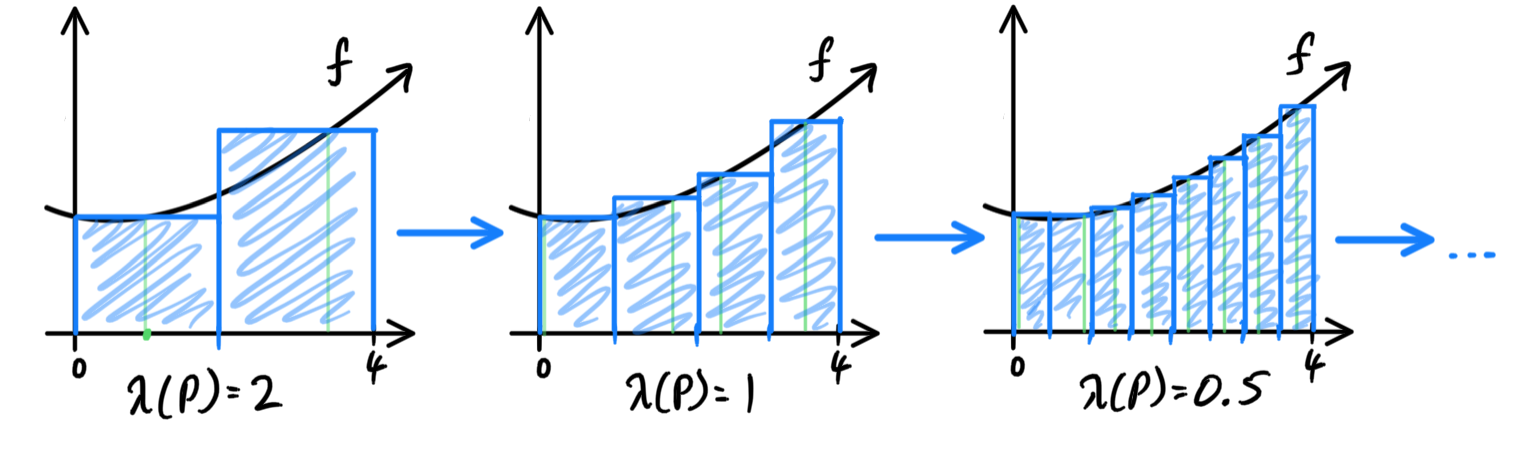
\includegraphics[scale=0.28]{img/Riemann_Integral_Limit_Mesh_goes_to_0.PNG}
      \end{center}
      Therefore, we can culminate by defining the Riemann integral of $f(x)$ over $[a,b]$ as 
      \[\int_a^b f(x)\,dx \equiv \lim_{\lambda(P) \rightarrow 0} \sum_{i=1}^n f(\xi_i) \lambda x_i\]
    \end{definition}

  \subsubsection{Conditions for Integrability}

    \begin{definition}[Riemann Integrable Functions]
      A function $f$ is \textbf{Riemann integrable} on the closed interval $[a, b]$ if 
      \[\int_a^b f(x)\,dx \equiv \lim_{\lambda(P) \rightarrow 0} \sum_{i=1}^n f(\xi_i) \lambda x_i\]
      is defined, i.e. if the limit of the right-hand side of Riemann sums exists as $\lambda(P) \rightarrow 0$ (that is, the Riemann integral of $f$ is defined). 

      Furthermore, the set of Riemann-integrable functions on a closed interval $[a, b]$ is denoted $\mathcal{R}[a,b]$. 
    \end{definition}

    Remember that the Riemann integral, as complicated as the formula is, is still a limit of a function. That means that we can apply the Cauchy criterion to it to determine convergence. 

    \begin{lemma}[Cauchy Criterion on Existence of Riemann Integral]
      Given a function $f$, the integral of $f$ over $[a, b]$, defined
      \[\int_a^b f(x)\,dx \equiv \lim_{\lambda(P) \rightarrow 0} \sum_{i=1}^n f(\xi_i) \lambda x_i\]
      exists if and only if for every $\epsilon>0$, there exists a $\delta>0$ such that 
      \[\big| \sigma(f; P^\prime, \xi^\prime) - \sigma(f; P^{\prime\prime}, \xi^{\prime\prime} \big| < \epsilon\]
      or, what is the same, 
      \[\Bigg| \sum_{i=1}^{n^\prime} f(\xi_i^\prime) \Delta x_i^\prime - \sum_{i=1}^{n^{\prime\prime}} f^(\xi_i^{\prime\prime}) \Delta x_i^{\prime\prime} \Bigg| < \epsilon\]
      for any partitions $(P^\prime, \xi^\prime)$ and $(P^{\prime\prime}, \xi^{\prime\prime})$ with distinguished points on the interval $[a, b]$ with
      \[\lambda(P^\prime), \lambda(P^{\prime\prime}) < \delta\]
      In words, this means that for any $\epsilon>0$ that we choose, there always exists a $\delta>0$ such that \textbf{any} two Riemann sums with mesh size \textbf{both} smaller than $\delta$ will have an error difference of less than $\epsilon$. \begin{center}
          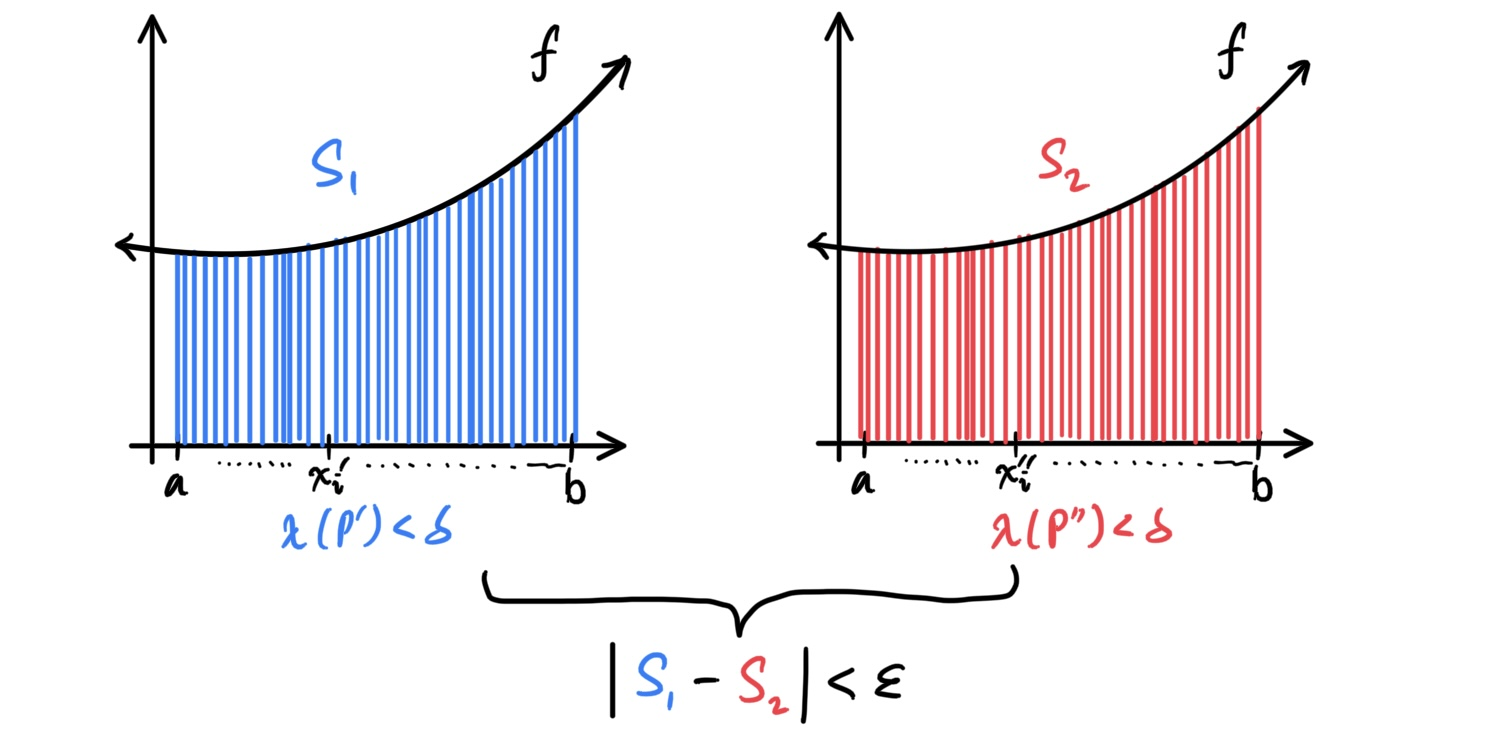
\includegraphics[scale=0.25]{img/Cauchy_Criterion_of_Riemann_Integral.jpg}
      \end{center}
    \end{lemma}

    \begin{theorem}[Necessary Condition for Integrability]
    A necessary condition for $f$ defined on a closed interval $[a, b]$ to be Riemann integrable on $[a, b]$ is that $f$ be bounded on $[a, b]$. That is, 
    \[f \in \mathcal{R}[a, b] \implies f \text{ is bounded on } [a, b]\]
    We can clearly see the necessity of $f$ being bounded by looking at the contrapositive of the following statement. 
    \end{theorem}

    \begin{theorem}[Refinement]
    Given a partition $P$ on interval $[a, b]$, recall that we have points $x_0, \ldots, x_n$ such that
    \[a = x_0 < x_1 < \ldots < x_n = b\]
    Here we introduce new notation: 
    \begin{enumerate}
      \item $\Delta_i$ denotes the interval $[x_{i-1}, x_i]$
      \item $\Delta x_i$ denotes the difference $x_i - x_{i-1}$, i.e. the length of $\Delta_i$
    \end{enumerate}
    If a partition $\Tilde{P}$ of the closed interval $[a, b]$ is obtained from the partition $P$ by the addition of new points to $P$, we call $\Tilde{P}$ a \textbf{refinement} of $P$. 

    When a refinement $\Tilde{P}$ of a partition $P$ is constructed, some (perhaps all) of the closed intervals $\Delta_i = [x_{i-1}, x_i]$ of the partition $P$ themselves undergo partitioning. 
    \[x_{i-1} = x_{i0} < x_{i1} < \ldots < x_{in_i} = x_i\]
    In that connection, it will be useful to label to points of $\Tilde{P}$ by double indices, where in the notation $x_{ij}$ the first index $i$ means that 
    \[x_{ij} \in \Delta_i = [x_{i-1}, x_i]\]
    and the second index $j$ is the ordinal number of the point on the closed interval $\Delta_i = [x_{i-1}, x_i]$. Therefore, it is natural to set the notations
    \begin{enumerate}
      \item $\Delta_{ij} = [x_{i j-1}, x_{ij}]$
      \item $\Delta x_{ij} = x_{ij} - x_{ij-1}$
    \end{enumerate}
    This means that 
    \[\Delta x_i = \Delta x_{i1} + \Delta x_{i2} + \ldots + \Delta x_{in_i}\]
    which can be visualized below
    \begin{center}
      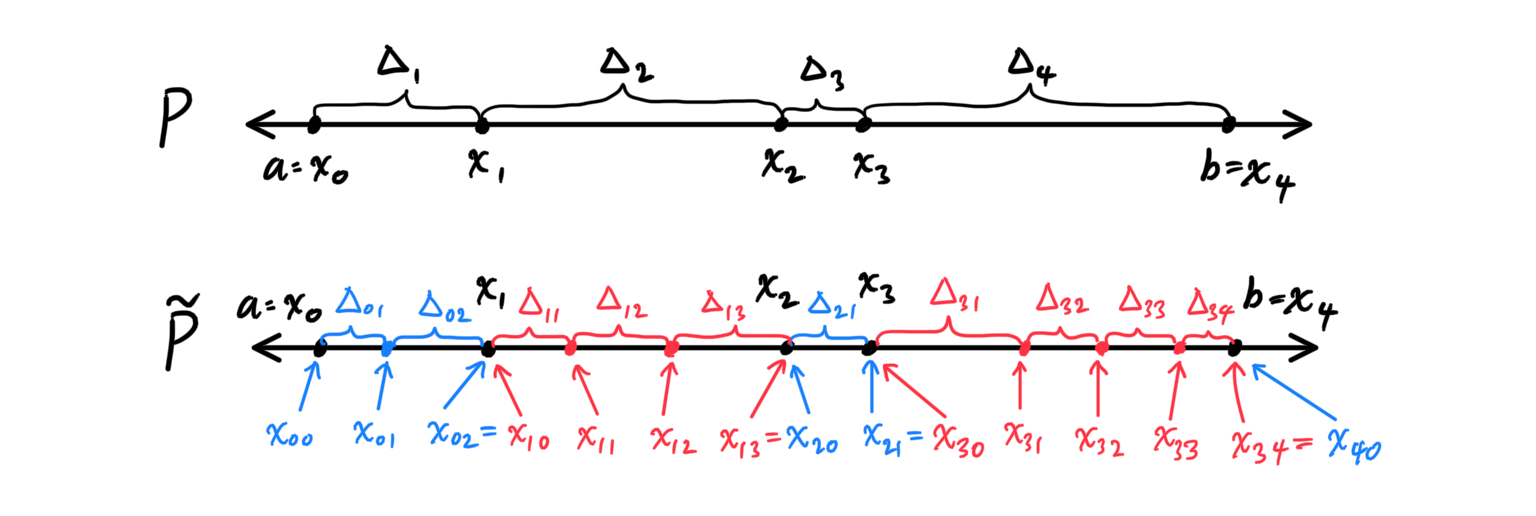
\includegraphics[scale=0.25]{img/Refinement_Definition_Analysis.PNG}
    \end{center}
    \end{theorem}

    \begin{example}[Union of Partitions as a Refinement]
    For some interval $[a, b]$, given partitions $P^\prime$ ($a = x_0 < \ldots < x_n = b$) and $P^{\prime\prime}$ ($a = y_0 < \ldots < y_n = b$), the union of the two partitions $\Tilde{P} = P^\prime \cup P^{\prime\prime}$ is a refinement of both $P^\prime$ and $P^{\prime\prime}$. 
    \begin{center}
        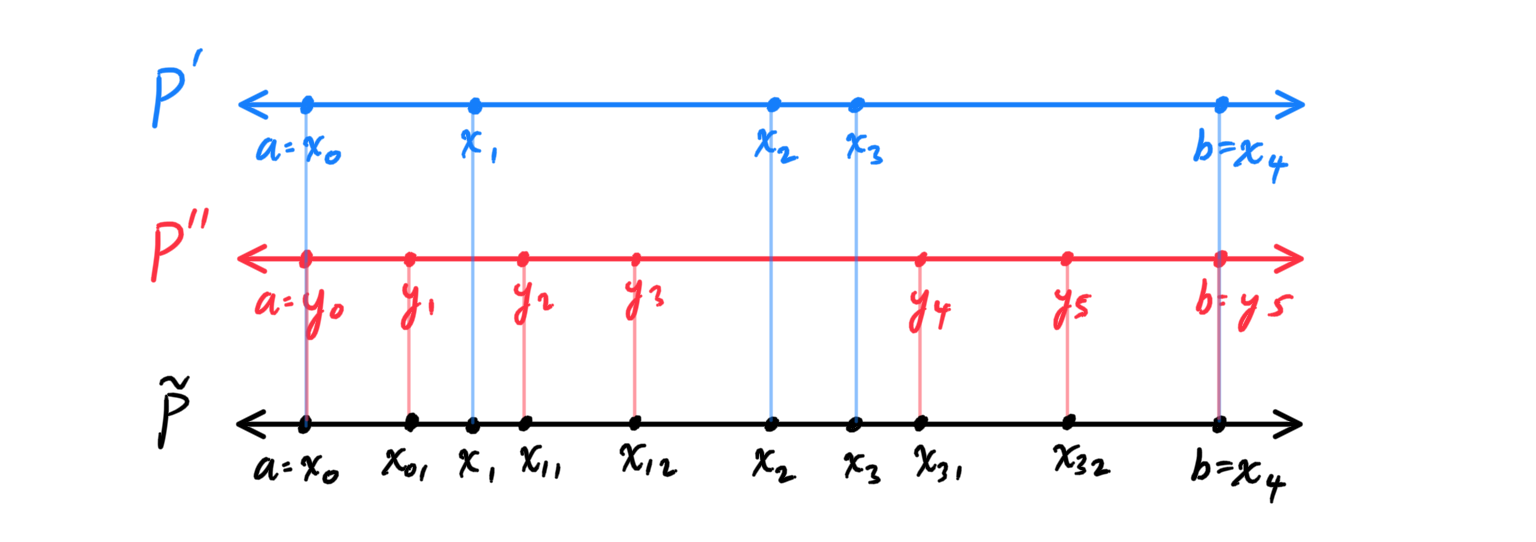
\includegraphics[scale=0.25]{img/Refinement_as_Union_of_Partitions.PNG}
    \end{center}
    \end{example}
    
    Recall that $\omega(f; E)$ denotes the oscillation of the function $f$ on the set $E$; that is, 
    \[\omega(f; E) \equiv \sup_{x^\prime, x^{\prime\prime} \in E} \big| f(x^\prime) - f(x^{\prime\prime})\big|\]
    In particular, $\omega(f; \Delta_i)$ is the oscillation of $f$ on the closed interval $\Delta_i$. 

    \begin{theorem}[Sufficient Condition for Integrability]
    Let $f$ be a bounded on a closed interval $[a, b]$ such that for every $\epsilon > 0$ there exists a number $\delta>0$ such that
    \[\sum_{i=1}^n \omega(f; \Delta_i) \Delta x_i < \epsilon\]
    for any partition $P$ of $[a, b]$ with mesh $\lambda(P) < \delta$. This is equivalent to saying that
    \[\lim_{\lambda(P) \rightarrow 0} \sum_{i = 1}^n \omega (f; \Delta_i) \, \Delta x_i = 0\]
    Then, $f$ is integrable. We can visualize
    \[\sum_{i=1}^n \omega(f; \Delta_i) \Delta x_i\]
    as the following sum of rectangles below. 
    \begin{center}
        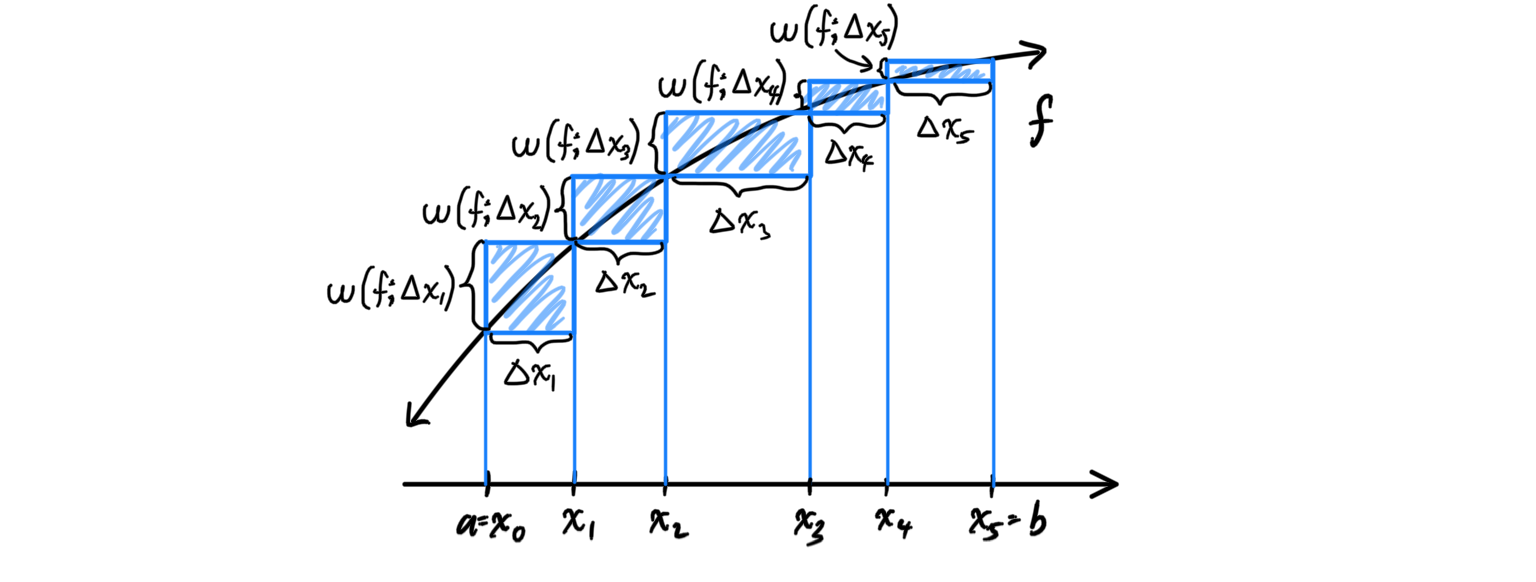
\includegraphics[scale=0.25]{img/Sufficient_Condition_for_Integrability.PNG}
    \end{center}
    What the theorem states, visually, is that as we make all the rectangles smaller and smaller (by putting a limit on the mesh $\lambda(P)<\delta$), we can make the sum of all these rectangles also arbitrarily small. 
    \end{theorem}

    \begin{corollary}[Integrability of Continuous Functions]
    Every continuous function on a closed interval is integrable on that closed interval. That is, 
    \[f \in C[a, b] \implies f \in \mathcal{R}[a, b]\]
    \end{corollary}

    We can actually make a stronger claim. 

    \begin{corollary}[Integrability of Discontinuous Functions]
    If a bounded function $f$ on a closed interval $[a, b]$ is continuous everywhere except at a finite set of points, then $f \in \mathcal{R}[a, b]$. 
    \end{corollary}

    \begin{corollary}[Integrability of Monotonic Functions]
    A bounded monotonic function on a closed interval is integrable on that interval. 
    \begin{center}
        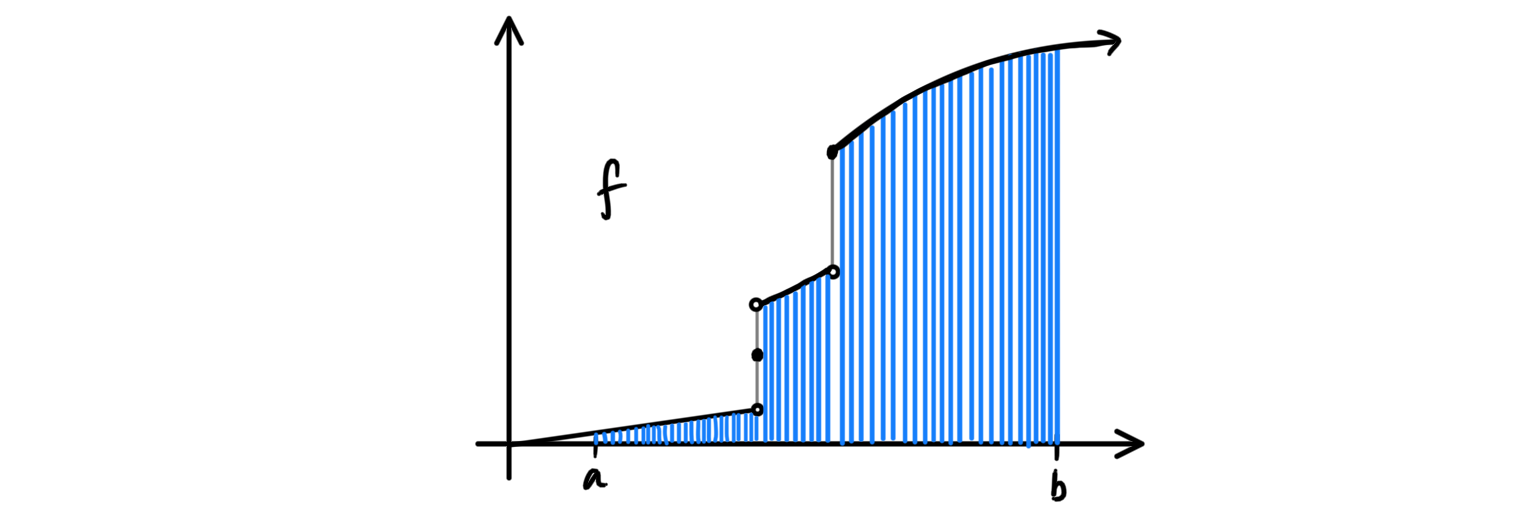
\includegraphics[scale=0.25]{img/Integrability_of_Monotonic_Function.PNG}
    \end{center}
    \end{corollary}

    \begin{definition}[Upper, Lower Riemann Sums]
      Let $f: [a, b] \longrightarrow \mathbb{R}$ be a real-valued function that is defined and bounded on the closed interval $[a, b]$, and let $P$ be a partition of $[a, b]$, and let $\Delta_i$ ($i = 1, 2, \ldots, n$) be the intervals of the partition $P$. Let 
      \begin{align*}
          m_i &= \inf_{x \in \Delta_i} f(x) \\
          M_i &= \sup_{x \in \Delta_i} f(x)
      \end{align*}
      be the infimum and supremum of $f$ over $\Delta x_i$. Then, the sums
      \begin{align*}
          s(f; P) & \equiv \sum_{i = 1}^n m_i \, \Delta x_i \\
          S(f; P) & \equiv \sum_{i=1}^n M_i \, \Delta x_i
      \end{align*}
      are respectively called the \textbf{lower} and \textbf{upper Riemann sums} of the function $f$ on the interval $[a, b]$ corresponding to the partition $P$ of that interval. 

      Given an arbitrary partition $(P, \xi)$ with distinguished points on $[a, b]$, it is clear that
      \[s(f; P) = \inf_{\xi} \sigma(f; P, \xi) \leq \sigma(f; P, \xi) \leq \sup_{\xi} \sigma(f; P, \xi) = S(f; P)\]
    \end{definition}

    \begin{theorem}
    A bounded real-valued function $f: [a, b] \longrightarrow \mathbb{R}$ is Riemann integrable on $[a, b]$ if and only if the following limits exist and are equal to each other. 
    \[\underline{I} \equiv \lim_{\lambda(P) \rightarrow 0} s(f; P) = \lim_{\lambda(P) \rightarrow 0} S(f; P) \equiv \overline{I}\]
    When the relation is true, then the integral is this common value. 
    \[\int_a^b f(x) \,dx = \underline{I} = \overline{I}\]
    \end{theorem}

    Note that this condition of the upper and lower Riemann sums converging to the same value and the condition that 
    \[\lim_{\lambda(P) \rightarrow 0} \sum_{i = 1}^n \omega (f; \Delta_i) \, \Delta x_i = 0\]
    are the same. For we can see that the rectangles visualized from the equation above are the exact same rectangles formed by $S(f; P) - s(f; P)$! 
    \begin{center}
        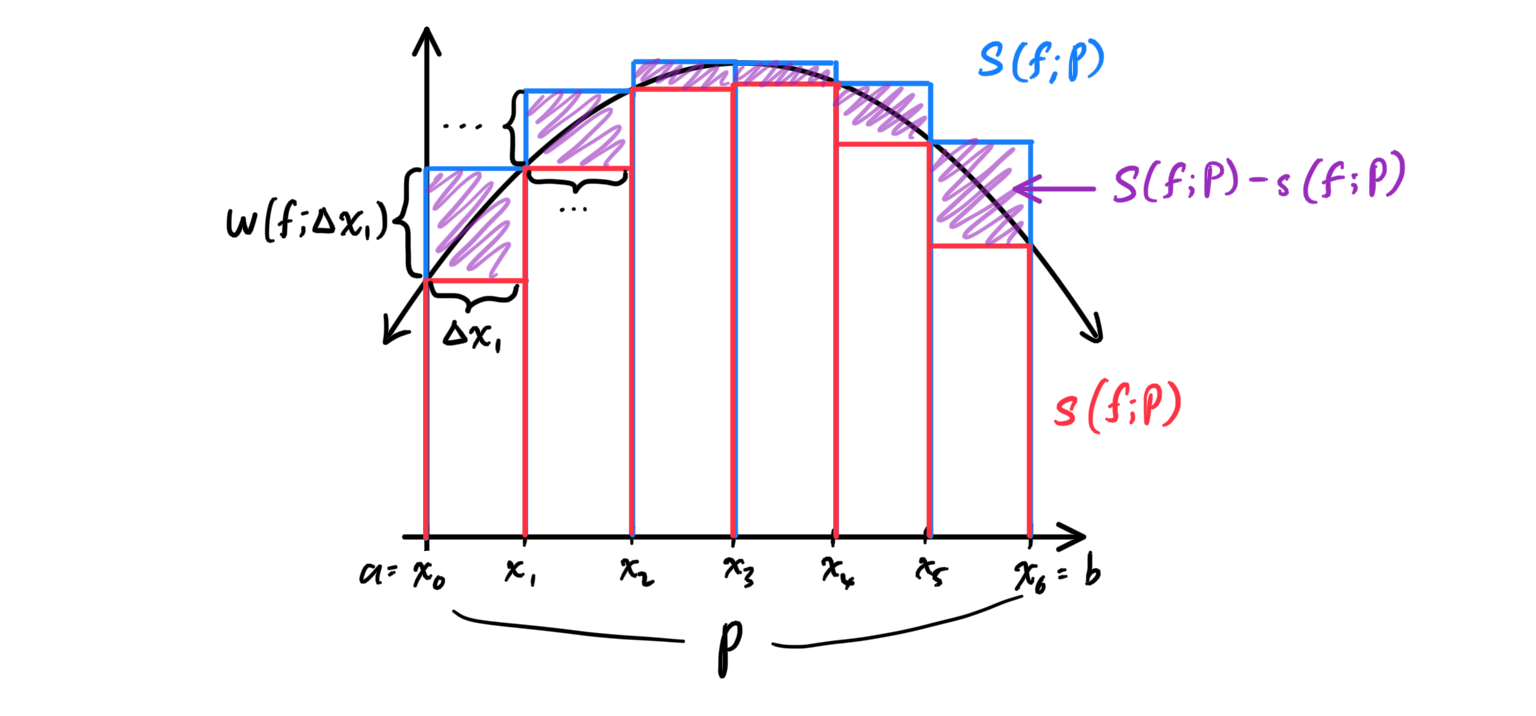
\includegraphics[scale=0.3]{img/Equivalent_Conditions_for_Integrability.PNG}
    \end{center}

    \subsubsection{The Vector Space of Riemann Integrable Functions}

    \begin{theorem}[The Vector Space of Integrable Functions]
    The set of Riemann integrable functions $\mathcal{R}[a, b]$ over closed interval $[a, b]$ is a vector space. That is, given $f, g \in \mathcal{R}[a, b]$ and $\alpha \in \mathbb{R}$, then
    \begin{enumerate}
      \item $(f + g) \in \mathcal{R}[a, b]$ 
      \item $(\alpha f) \in \mathcal{R}[a, b]$
    \end{enumerate}
    Furthermore, 
    \begin{enumerate}
      \item $|f| \in \mathcal{R}[a, b]$
      \item The restriction of $f$ in any $[c, d] \subset [a, b]$, denoted $f \big|_{[c,d]}$, is in $\mathcal{R}[c,d]$
      \item $(f \cdot g) \in \mathcal{R}[a, b]$
    \end{enumerate}
    \end{theorem}
    \begin{proof}

    \end{proof}

    \subsubsection{Lebesgue's Criterion for Riemann Integrability}
    We give Lebesgue's version of an intrinsic description of a Riemann integrable function. 

    \begin{definition}[Measure]
      A set $E \subset \mathbb{R}$ has \textbf{(Lebesgue) measure zero} if for every number $\epsilon > 0$ there exists a covering of the set $E$ be an at most countable system $\{I_k\}$ of intervals, the sum of whose lengths 
      \[\sum_{k=1}^\infty |I_k| \leq \epsilon\]
      This means that the above series summing up the lengths of the intervals is an absolutely convergent series. 
    \end{definition}

    \begin{lemma}
      We can deduce measures of basic sets. 
      \begin{enumerate}
        \item A finite number of points are sets of measure zero. 
        \item The union of a finite or countable number of sets of measure zero is a set of measure zero. \item A subset of a set of measure zero is itself a set of measure zero. 
        \item A closed interval $[a, b]$ with $a<b$ is not a set of measure zero. 
      \end{enumerate}
    \end{lemma}

    \begin{definition}
      If a property holds at all points of a set $X$ except possible the points of a set of measure zero, we say that this property holds \textbf{almost everywhere on $X$} or \textbf{at almost every point of $X$}. 
    \end{definition}

    Now, we can state Lebesgue's criterion for integrability, which nicely summarizes what we have so far. 

    \begin{theorem}[Lebesgue's Criterion for Integrability]
    A function defined on a closed interval is Riemann integrable on that interval if and only if it is bounded and continuous at almost every point. 
    \end{theorem}

    \begin{example}[Non-Integrability of the Dirichlet Function]
    The Dirichlet function
    \[\mathcal{D}(x) \equiv \begin{cases}
    1, & \text{ for } x \in \mathbb{Q} \\
    0, & \text{ for } x \in \mathbb{R} \setminus \mathbb{Q}
    \end{cases}\]
    on the interval $[0,1]$ is not integrable on that interval. We state two different reasons why. 
    \begin{enumerate}
      \item For any partition $P$ of $[0,1]$ we can find in each interval $\Delta_i$ both a rational point $\xi^\prime_i$ and an irrational point $\xi_i^{\prime\prime}$. Then, we can see that the lower and upper Riemann sums do not necessarily converge to each other since
      \[\sigma(f; P, \xi^\prime) = \sum_{i=1}^n 1 \cdot \Delta x_i = 1 \text{ while } \sigma(f;P, \xi^{\prime\prime}) = \sum_{i=1}^n 0 \cdot \Delta x_i = 0\]
      as $\lambda(P) \rightarrow 0$. 
      \item From the point of view of the Lebesgue criterion the nonintegrability of the Dirichlet function is obvious since $\mathcal{D}(x)$ is discontinuous at every point of $[0, 1]$, which is not a set of measure zero. 
    \end{enumerate}
    \end{example}

    Notice that by the Lebesgue criterion, integrability is a weaker condition than continuity. That is, 
    \[f \text{ continuous } \implies f \text{ Riemann integrable}\]
    but not necessarily the other way around. It turns out that this has consequences when determining the composition of functions. 

    \begin{proposition}[Integrable + Continuous Composition]
    Let $f: I_1 = [a, b] \longrightarrow\mathbb{R}$ be a function that is integrable on $[a, b]$, with Im$\,f = [c, d] = I_2$. Define a continuous (remember, continuity is stronger than integrability) function $g: [c, d] \longrightarrow \mathbb{R}$. Then the composition
    \[g \circ f: [a, b] \longrightarrow \mathbb{R}\]
    is clearly defined and continuous at all the points of $[a, b]$ where $f$ is continuous. But since $f$ is integrable, the union of all the discontinuities in $[a, b]$ must have measure zero, and so it follows that since $[a, b]$ is the same  
    \[g \circ f \in \mathcal{R}[a, b]\]
    Therefore, we can found out that 
    \[f \text{ integrable and } g \text{ continuous} \implies g \circ f \text{ integrable}\]
    as visualized in the commutative diagram below. 
    \[
      \begin{tikzcd}
        I_1 \arrow[r, "f"] \arrow[rr, bend left, "g \circ f"] & I_2 \arrow[r, "g"] & \mathbb{R}
      \end{tikzcd}
    \]
    However, contrary to intuition, 
    \[f \text{ integrable and } g \text{ integrable} \centernot\implies g \circ f \text{ integrable}\]
    \end{proposition}

    We present a counterexample. 
    \begin{example}
    Consider the functions
    \[|sgn|(x) \equiv \begin{cases}
    1 & x \neq 0 \\
    0 & x = 0
    \end{cases}\]
    and the Riemann function 
    \[\mathcal{R}(x) \equiv \begin{cases}
    \frac{1}{n} & x = \frac{m}{n} \in \mathbb{Q}, \gcd(m, n) = 1 \\
    0 & x \in \mathbb{R} \setminus \mathbb{Q}
    \end{cases}\]
    We can see that $\mathcal{R}$ is continuous at all irrational points and discontinuous at all rational points except $0$, meaning that it is integrable ($\mathbb{Q}$ has measure zero). Then, the composition of these two functions is precisely the Dirichlet function
    \[\mathcal{D}(x) = |sgn| \circ \mathcal{R}\]
    which is not integrable. 
    \end{example}

  \subsection{Basic Properties of the Integral}

    One of the most basic properties of the integral is that it is a linear map. 
    \begin{lemma}[Linearity of the Integral]
      Given closed interval $[a, b] \subset \mathbb{R}$, the Riemann integration function 
      \[\int_a^b: \mathcal{R}[a, b] \longrightarrow \mathbb{R}\]
      is a linear functional living within the dual space $\mathbb{R}^* [a, b]$. That is, given $f, g \in \mathcal{R}[a, b]$, a linear combination of them $\alpha f + \beta g$ is also integrable on $[a,b]$, and 
      \[\int_a^b (\alpha f + \beta g)(x)\,dx = \alpha \int_a^b f(x)\,dx + \beta \int_a^b g(x)\,dx\]
    \end{lemma}
    \begin{proof}
    It is clear from basic algebraic transformation that the Riemann sums for the integral expressions on both sides are equal. 
    \[\sum_{i=1}^n (\alpha f + \beta g) (\xi_i) \Delta x_i = \alpha \sum_{i=1}^n f(\xi_i) \Delta x_i + \beta \sum_{i=1}^n g(\xi_i) \Delta x_i\]
    Taking the limit as $\lambda(P) \rightarrow 0$ on both sides leads to the respective Riemann integrals. 
    \end{proof}


    The next property of the Riemann integral is its additive property \textbf{on the interval of integration}. Note that the value of the integral 
    \[\int_a^b f(x) \,dx \equiv \lim_{\lambda(P) \rightarrow 0} \sigma(f; P, \xi)\]
    depends on both the integrand and the closed interval over which the integral is taken. 

    \begin{lemma}[Properties of the Interval of Integration]
      If $a < b < c$ and $f \in \mathcal{R}[a, c]$, then $f \big|_{[a,b]} \in \mathcal{R}[a, b]$, $f \big|_{[b,c]} \in \mathcal{R}[b, c]$, and the following equality holds 
      \[\int_a^c f(x)\,dx = \int_a^b f(x)\, dx + \int_b^c f(x)\,dx\]
      From these we set
      \[\int_a^b f(x)\,dx \equiv - \int_b^a f(x)\,dx\]
      and 
      \[\int_a^a f(x)\,dx \equiv 0\]
    \end{lemma}

    \begin{theorem}[Symmetry of the Riemann Integral]
    Let $a, b, c \in \mathbb{R}$ and let $f$ be integrable over the largest closed interval having two of these points as endpoints. Then, the restriction of $f$ to each of the other closed intervals is also integrable over those intervals and the following equality holds. 
    \[\int_a^b f(x)\,dx + \int_b^c f(x)\,dx + \int_c^a f(x)\,dx = 0\]
    This property can be abstractified to those of additive interval functions, which will be shown soon. 
    \end{theorem}

    We finally end with an important property of the integral which, as seen later, allows us to define inner products on function spaces. 
    \begin{theorem}
    If $a \leq b$ and $f \in \mathcal{R}[a, b]$, then $|f| \in \mathcal{R}[a, b]$, and 
    \[\Bigg| \int_a^b f(x)\,dx \Bigg| \leq \int_a^b |f|(x)\,dx\]
    \end{theorem}

    \subsubsection{Mean Value Theorem of the Integral}

    \begin{lemma}[Monotonicity of the Integral]
      If $a \leq b, f_1, f_2 \in \mathcal{R}[a, b]$, and $f_1 (x) \leq f_2 (x)$ for every $x \in [a, b]$, then
      \[\int_a^b f_1 (x)\,dx \leq \int_a^b f_2 (x)\,dx\]
      \begin{center}
          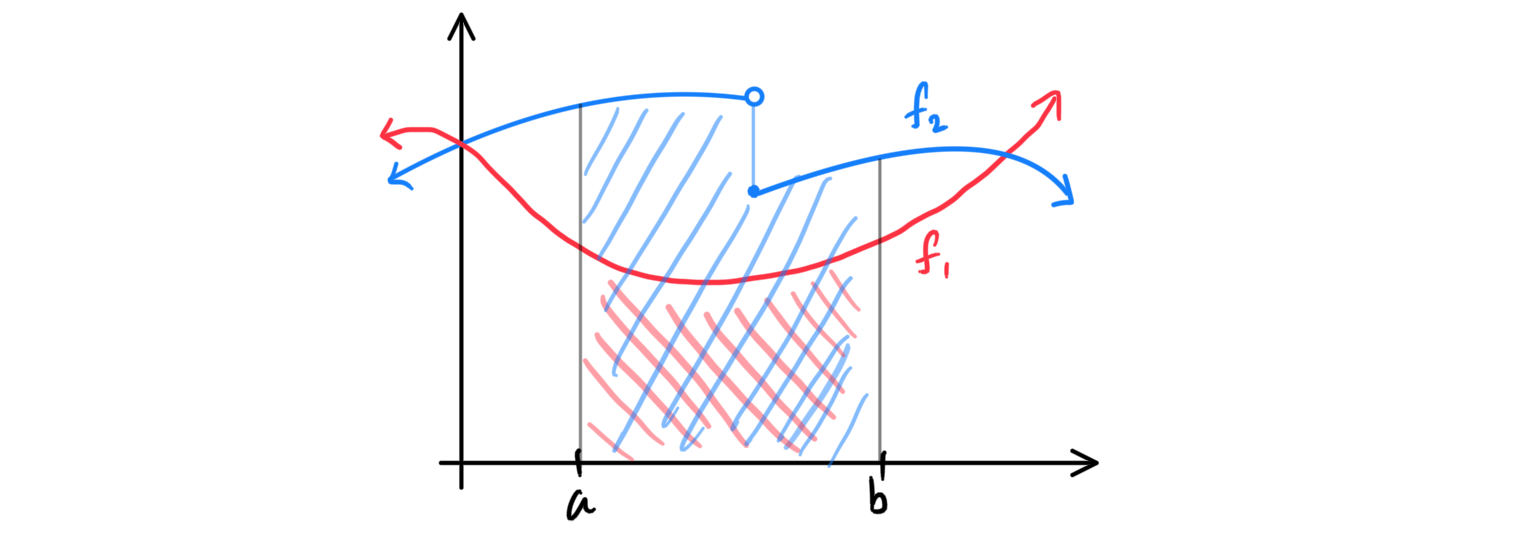
\includegraphics[scale=0.27]{img/Monotonicity_of_Integral.PNG}
      \end{center}
      This immediately implies that given constants $m, M$ such that $m \leq f(x) \leq M$ at each $x \in [a, b]$, we have
      \[m \cdot (b - a) \leq \int_a^b f(x)\,dx \leq M \cdot (b-a)\]
      This is very easily visualized below. 
      \begin{center}
          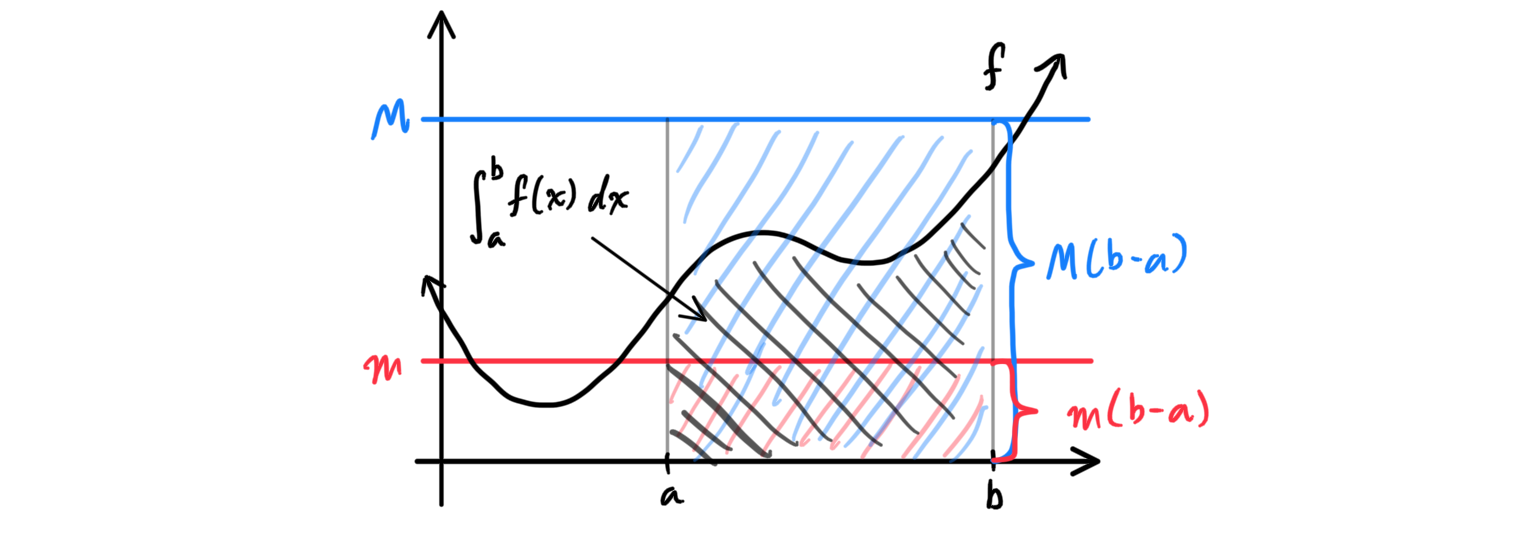
\includegraphics[scale=0.27]{img/Monotonicity_of_Intergral_2.PNG}
      \end{center}
      In particular, if $0 \leq f(x)$ on $[a, b]$, then
      \[0 \leq \int_a^b f(x)\,dx\]
    \end{lemma}

    \begin{theorem}[Mean Value Theorem of the Integral]
    Given $f \in \mathcal{R}[a, b]$, with 
    \[m = \inf_{x \in [a, b]} f(x) \text{ and } M = \sup_{x \in [a, b]} f(x)\]
    then there exists a number $\mu \in [m, M]$ such that
    \[\int_a^b f(x)\,dx = \mu \cdot (b - a)\]
    Furthermore, if $f \in C[a, b]$ (that is, continuous on $[a, b]$), it immediately follows by the intermediate value theorem that there exists a point $\xi \in [a, b]$ such that
    \[\int_a^b f(x)\,dx = f(\xi) (b - a)\]
    \begin{center}
        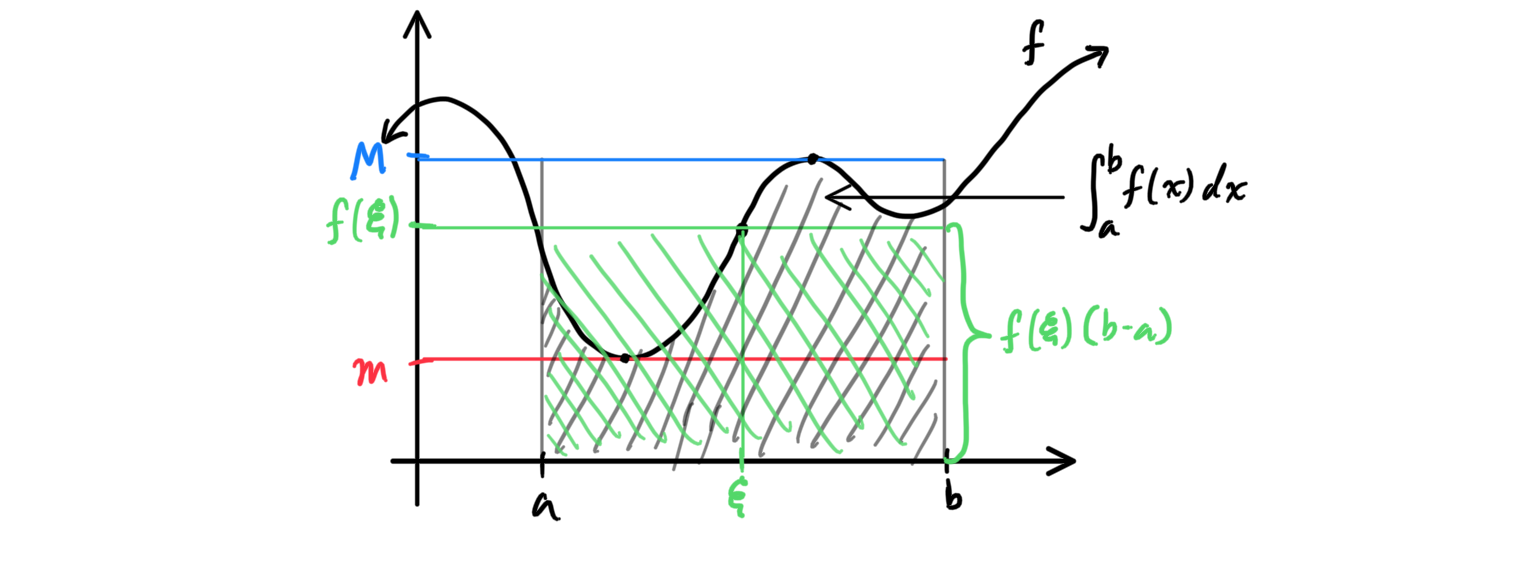
\includegraphics[scale=0.27]{img/Mean_Plus_Intermediate_Value_Theorem_Integral.PNG}
    \end{center}
    \end{theorem}

    Due to the length of the proof, we ask the reader to take it for granted the following theorem. 

    \begin{theorem}[Bonnet's Formula]
    If $f, g \in \mathcal{R}[a, b]$ and $g$ is a monotonic function on $[a, b]$, then there exists a point $\xi \in [a, b]$ such that
    \[\int_a^b (f \cdot g) (x)\,dx = g(a) \int_a^\xi f(x)\,dx + g(b) \int_\xi^b f(x)\,dx\]
    \end{theorem}

  \subsection{Connections between Integrals, Primitives, Derivatives}

    \begin{definition}[Integral with Variable Upper Limit]
      Let $f \in \mathcal{R}[a, b]$, and let us choose an $x \in [a, b]$ in order to construct the function
      \[F(x) \equiv \int_a^x f(t)\,dt\]
      which is called an \textbf{integral with variable upper limit}. Note that since $[a, x] \subset [a, b]$, it follows that $f \big|_{[a,x]} \in \mathcal{R}[a, x]$ and therefore the function $x \mapsto F(x)$ is unambiguously defined for $x \in [a, b]$. 
      \begin{center}
          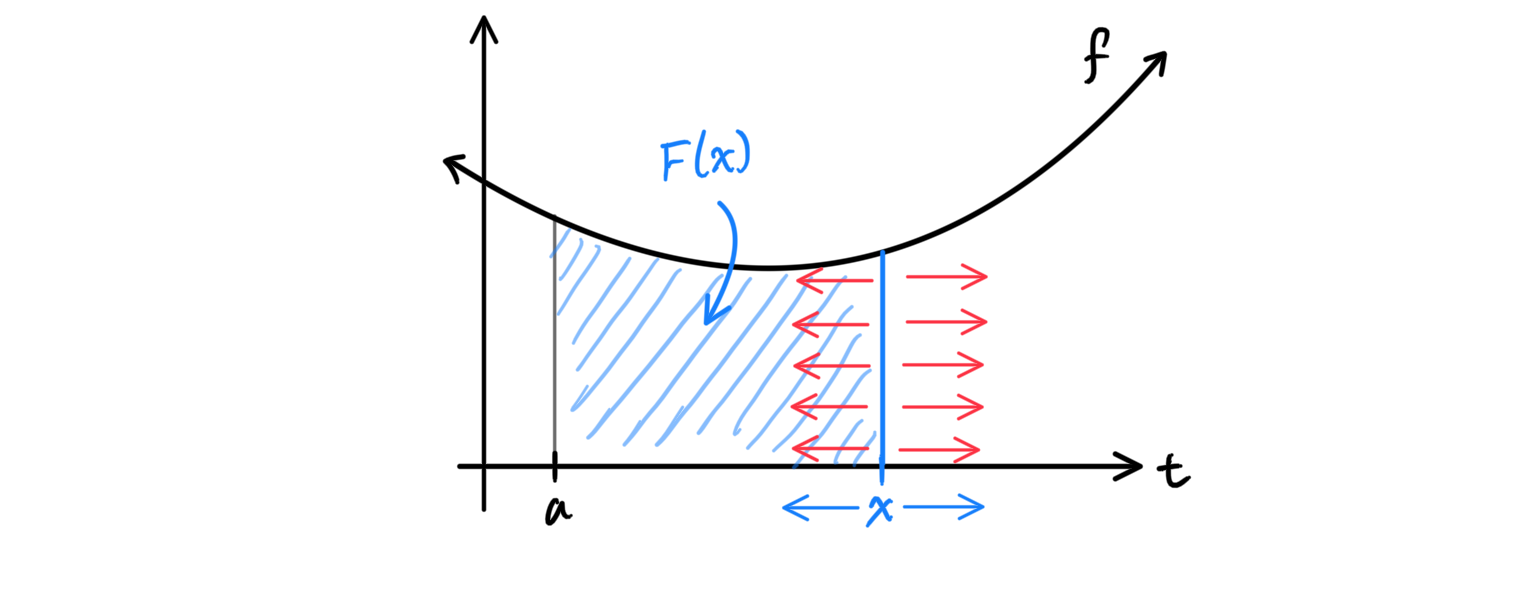
\includegraphics[scale=0.27]{img/Integral_with_Variable_Upper_Limit.PNG}
      \end{center}
      Furthermore, $F(x)$ is continuous on $[a, b]$. Since $f$ is integrable on $[a, b]$, it is bounded by a constant $C$ such that
      \[|f(t)| \leq C \text{ on } [a, b]\]
      It follows from the additive properties of the integral and boundedness theorem that 
      \[|F(x + h) - F(x)| \leq C|h|\]
      if $x, x + h \in [a, b]$, as visualized. This means that for any $\delta$-neighborhood of $F(x)$, we can find an arbitrary small $h$ such that the $C|h|$-neighborhood of $F(x)$ is completely contained in the $\delta$-neighborhood. But by the inequality above, this means that there exists an $\epsilon = h$-neighborhood of $x$ such that its entire image is contained within the $C|h|$-neighborhood, which itself is contained within the $\delta$-neighborhood. This shows that $F$ is continuous. 
    \end{definition}

    \begin{theorem}[First Fundamental Theorem of Calculus]
    Let $f \in \mathcal{R}[a, b]$ be continuous at point $x \in [a, b]$ (resp. continuous on closed interval $[a, b]$). Let $F$ be the function, defined for all $x \in [a, b]$ by 
    \[F(x) \equiv \int_a^x f(t)\,dt\]
    Then, $f$ is continuous and differentiable at $x$ (resp. uniformly continuous on $[a, b]$ and differentiable on $(a, b)$), 
    \[F^\prime (x) = f(x)\]
    at $x$ (resp. for all $x \in [a, b]$). This is an amazing fact, because visually, it tells us that the rate at which the integral $F$ is increasing at $x$ (represented by the increasing area under the curve of $f$) is equal to the value of $f$ at the point $x$ itself! 
    \begin{center}
        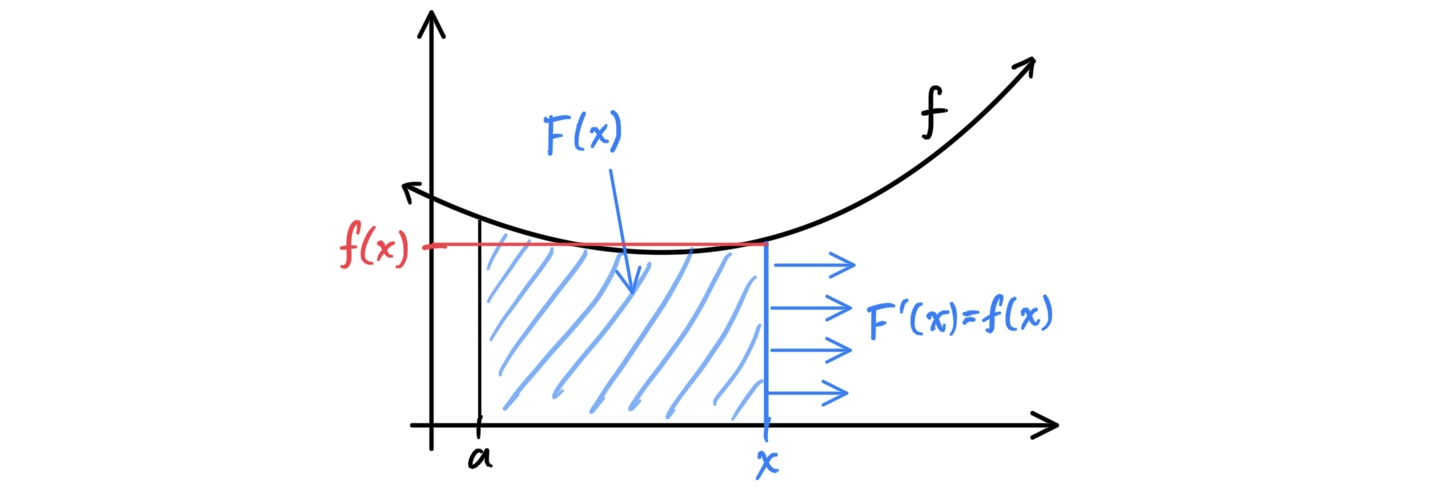
\includegraphics[scale=0.25]{img/First_Fundamental_Theorem_Analysis.jpg}
    \end{center}
    \end{theorem}
    \begin{proof}
    Let $x, x + h \in [a, b]$, and let us estimate the difference $F(x+h) - F(x)$. It follows from the continuity of $f$ at $x$ that $f(t) = f(x) + \Delta(t)$, where $\Delta(t) \rightarrow 0$ as $t \rightarrow x$. If point $x$ is held fixed, the function 
    \[\Delta(t) = f(t) - f(x)\]
    is integrable on $[a, b]$, being the difference of the integrable function $t \mapsto f(t)$ and the constant $f(x)$. Let us denote
    \[M(h) \equiv \sup_{t \in [x, x+h]} |\Delta(t)|\]
    which means that $M(h)$ is the largest difference between $f(x)$ and $f(t)$ in the interval $[x, x+h]$. 
    \begin{center}
        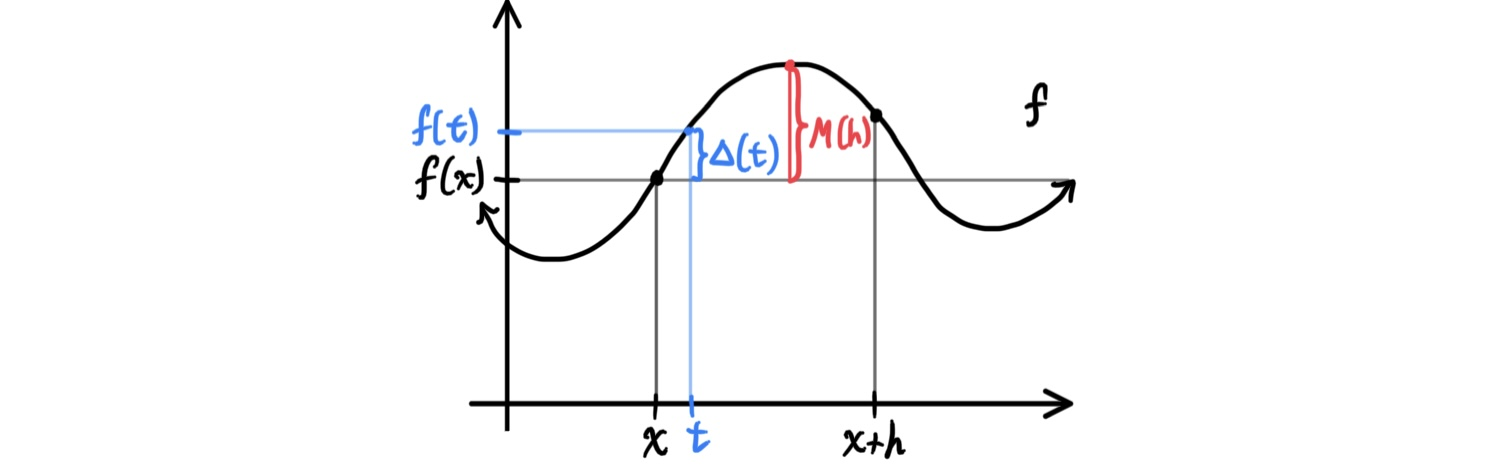
\includegraphics[scale=0.25]{img/Proof_First_Fundamental_Theorem_Analysis.jpg}
    \end{center}
    Clearly $M(h) \rightarrow 0$ as $h \rightarrow 0$. We can now find
    \begin{align*}
        F(x + h) - F(x) & = \int_a^{x+h} f(t)\,dt - \int_a^x f(t)\,dt \\
        & = \int_x^{x+h} f(t)\,dt \\
        & = \int_x^{x+h} \big( f(x) + \Delta(t)\big)\,dt \\
        & = \int_x^{x+h} f(x)\,dt + \int_x^{x+h} \Delta(t)\,dt \\
        & = f(x) h + \alpha(h) h
    \end{align*}
    where we have set 
    \[\int_x^{x+h} \Delta(t)\,dt = \alpha(h) h\]
    where $\alpha$ is infinitesimal as $h \rightarrow 0$, since 
    \[\Bigg| \int_x^{x+h} \Delta(t)\,dt \Bigg| \leq \Bigg| \int_x^{x+h} |\Delta(t)|\,dt \Bigg| \leq \Bigg| \int_x^{x+h} M(h)\,dt \Bigg| = M(h) |h| = \alpha(h)|h|\]
    Therefore, we have shown that if the function $f$ is continuous at a point $x \in [a, b]$, then for displacements $h$ from $x$ such that $x +h \in [a, b]$, the following equality holds.
    \[F(x + h) - F(x) = f(x) h + \alpha(h) h\]
    where $\alpha(h) \rightarrow 0$ as $h \rightarrow 0$, and by definition, this means that $F(x)$ is differentaible on $[a, b]$ at the point $x \in [a, b]$ and that $F^\prime(x) = f(x)$. 
    \end{proof}

    \begin{corollary}
    Every bounded function $f: [a, b] \longrightarrow \mathbb{R}$ on the closed interval $[a, b]$ and has only a finite number of points of discontinuity has a primitive, and every primitive of $f$ on $[a, b]$ has the form 
    \[\mathcal{F}(x) \equiv \int_a^x f(t)\,dt + c\]
    where $c$ is a constant. 
    \end{corollary}

    \begin{theorem}[Second Fundamental Theorem of Calculus]
    Let $f$ be a real-valued function on a closed interval $[a, b]$ with $\mathcal{F}$ any primitive of $f$ on $[a, b]$. If $f$ is Riemann-integrable (i.e. $f$ bounded with finite points of Lebesgue measure zero) on $[a, b]$, then 
    \[\int_a^b f(x)\,dx  = \mathcal{F} \big|_a^b \equiv \mathcal{F}(b) - \mathcal{F}(a)\]
    \begin{center}
        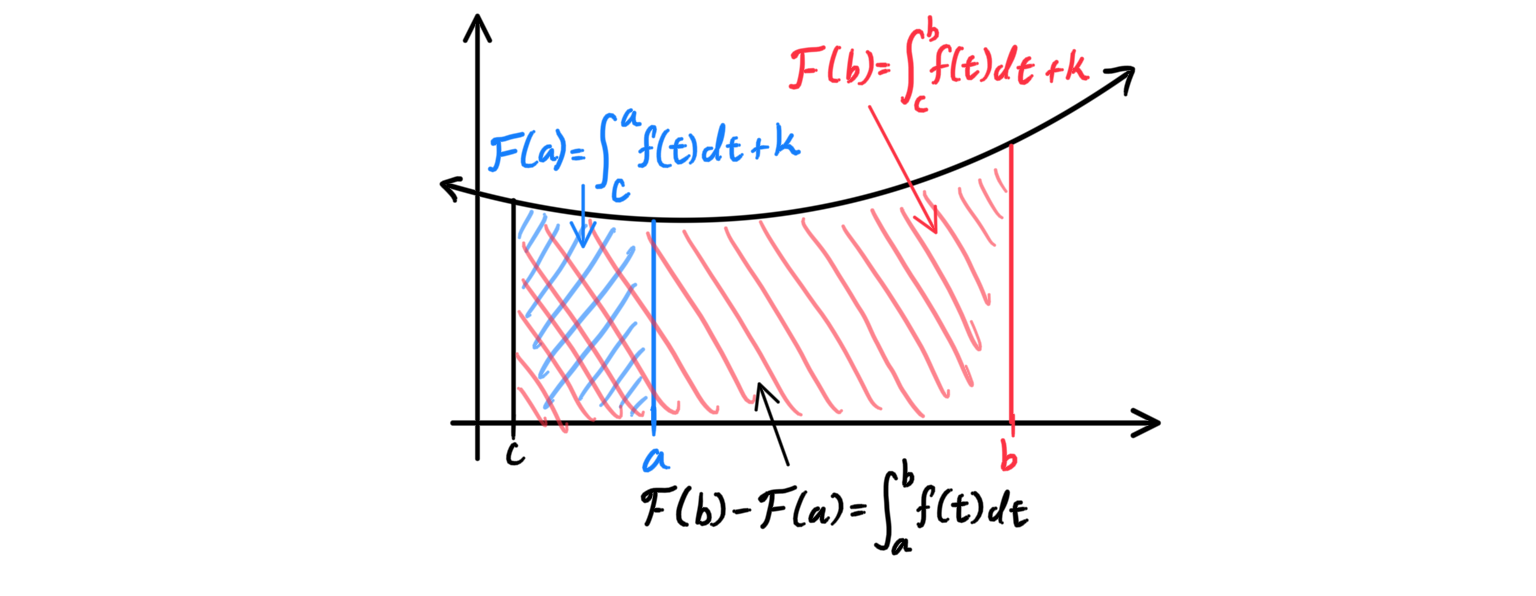
\includegraphics[scale=0.25]{img/Second_Fundamental_Theorem_Analysis.PNG}
    \end{center}
    \end{theorem}
    \begin{proof}
    We already know that a bounded function on a closed interval having a finite number of discontinuities is integrable, and by the corollary, we are guaranteed an existence of a primitive $\mathcal{F}(x)$ of the function $f$ on $[a, b]$ with the form 
    \[\mathcal{F} (x) \equiv \int_a^x f(t)\,dt + c\]
    Setting $x = a$, we find that $c = \mathcal{F}(a)$, and so 
    \[\mathcal{F}(x) \equiv \int_a^x f(t)\,dt + \mathcal{F}(a)\]
    Evaluating $\mathcal{F}$ at $x = b$ gives
    \[\int_a^b f(t)\,dt = \mathcal{F}(b) - \mathcal{F}(a)\]
    \end{proof}

    \subsubsection{Integration by Parts and Taylor's Formula}
    \begin{theorem}[Definite Integration by Parts]
    If the functions $u(x)$ and $v(x)$ are continuously differentiable on a closed interval with endpoints $a$ and $b$, then
    \[\int_a^b (u \cdot v^\prime)(x)\,dx = (u \cdot v)\big|^b_a - \int_a^b (v \cdot u^\prime)(x)\,dx\]
    which is customarily written in the form as
    \[\int_a^b u\,dv = u \cdot v \big|_a^b - \int_a^b v\,du\]
    \end{theorem}
    \begin{proof}
    By the product rule of differentiation, we have
    \[(u \cdot v)^\prime (x) = (u^\prime \cdot v)(x) + (u \cdot v^\prime) (x)\]
    where by hypothesis, $u^\prime \cdot v, u \cdot v^\prime$ are continuous and hence integrable on $[a, b]$. Using the linearity of the integral and the 2nd fundamental theorem of calculus, we get
    \[(u \cdot v) (x) \big|^b_a = \int_a^b (u^\prime \cdot v)(x)\,dx + \int_a^b (u \cdot v^\prime) (x)\,dx\]
    \end{proof}

    \begin{theorem}[Integral Form of the Remainder]
    If $f: E \longrightarrow \mathbb{R}$ has continuous derivatives up to order $n$ on the closed interval $[a, x]$, then Taylor's formula holds
    \[f(x) = f(a) + \frac{f^\prime (a)}{1!} (x - a) + \ldots + \frac{f^{(n-1)}(a)}{(n-1)!} (x - a)^{n-1} + r_{n-1}(a; x)\]
    where 
    \[r_{n-1} (a;x) = \frac{1}{(n-1)!} \int_a^x f^{(n)} (t) (x - t)^{n-1} \,dt\]
    This form is called \textbf{Taylor's formula with the integral form of the remainder}. 
    \end{theorem}
    \begin{proof}
    Using the 2nd fundamental theorem and the definite integration by parts formula, we can carry out the following chain of transformations, assuming continuity and differentiability when needed. 
    \begin{align*}
        f(x) - f(a) & = \int_a^x f^\prime (t) \,dt \\
        & = - \int_a^x f^\prime(t) (x - t)^\prime \,dt \\
        & = -f^\prime (t) (x - t)\big|_a^x + \int_a^x f^{\prime\prime} (t) (x - t) \,dt \\
        & = f^\prime (a) (x - a) - \frac{1}{2} \int_a^x f^{\prime\prime} (t) \big( (x - t)^2\big)^\prime \,dt \\
        & = f^\prime (x - a) - \frac{1}{2} f^{\prime\prime} (t) (x - t)^2 \big|_a^x + \frac{1}{2} \int_a^x f^{\prime\prime\prime} (t) (x - t)^2\,dt \\
        & = f^\prime(a) (x - a) + \frac{1}{2} f^{\prime\prime} (a) (x - a)^2 - \frac{1}{2 \cdot 3} \int_a^x f^{\prime\prime\prime} (t) \big((x - t)^3\big)^\prime\,dt \\
        & = \ldots \\
        & = f^\prime (a) (x - a) + \ldots + \frac{1}{(n-1)!} f^{(n-1)} (a)(x - a)^{n-1} + r_{n-1}(a;x)
    \end{align*}
    where $r_{n-1}(a;x)$ is given by the integral formula mentioned. 
    \end{proof}

    \subsubsection{Change of Variables in Integration}
    We now show and prove the method what we call "u-substitution" for definite integration. 

    \begin{theorem}[Change of Variable]
    If $\varphi: [\alpha, \beta] \longrightarrow [a, b]$ is a continuously differentiable mapping such that $\varphi(\alpha) = a$ and $\varphi(\beta) = b$, then for any continuous function $f(x)$ on $[a, b]$ the function $f\big(\varphi(t)\big) \varphi^\prime (t)$ is continuous on the closed interval $[\alpha, \beta]$ and 
    \[\int_a^b f(x)\,dx = \int_\alpha^\beta f\big(\varphi(t)\big) \varphi^\prime(t)\,dt\]
    \begin{center}
        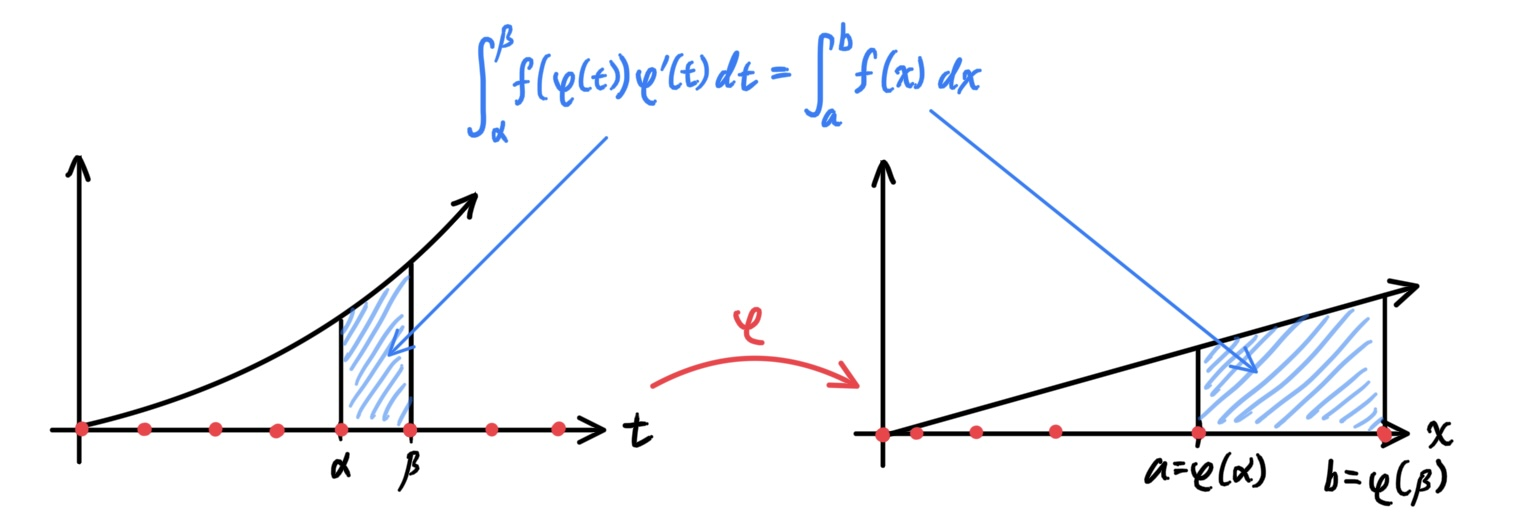
\includegraphics[scale=0.25]{img/Change_of_Variable_Analysis_Integral.jpg}
    \end{center}
    \end{theorem}
    \begin{proof}
    We prove a slightly weaker form of the theorem with the additional hypothesis that $\varphi$ is strictly monotonic. 
    \end{proof}

    \subsubsection{Additive Interval Functions and the Integral}
    In this section we take a step back and construct the integral in a more abstract sense, using the concepts of an additive interval function. 

    \begin{definition}[Additive Interval Function]
      An \textbf{additive (oriented) interval function} is a function 
      \[(\alpha, \beta) \mapsto I(\alpha, \beta) \in \mathbb{R}\]
      that assigns a number $I(\alpha, \beta)$ to each ordered pair of points $(\alpha, \beta)$ of a fixed closed interval $[a, b]$ in such a way that the following equality holds for any triple of points $\alpha, \beta, \gamma \in [a, b]$. 
      \[I(\alpha, \gamma) = I(\alpha, \beta) + I(\beta, \gamma)\]
      Notice that the integral holds this property, shown in the theorem on the symmetric property of the integral. It follows that all additive interval functions are anticommutative: 
      \[I(\alpha, \beta) + I(\beta, \alpha) = 0\]
      which immediately results in
      \[I(\alpha, \alpha) = 0\]
    \end{definition}

    \begin{lemma}[Generating Functions of Additive Interval Functions]
      For any function $x \mapsto \mathcal{F}(x)$ that maps points on the interval $[a, b]$ to $\mathbb{R}$, we set
      \[\mathcal{F}(x) \equiv I(a, x)\]
      and by additivity we have
      \[I(\alpha, \beta) = I(\alpha, \beta) - I(a, \alpha) = \mathcal{F}(\beta) - \mathcal{F}(\alpha)\]
      and thus, every additive oriented interval function has the form 
      \[I(\alpha, \beta) = \mathcal{F}(\beta) - \mathcal{F}(\alpha)\]
      By constructing $I$ in this manner, we say that \textbf{the function $\mathcal{F}$ generates the additive function $I$}. 
    \end{lemma}

    \begin{example}
    If $f \in \mathcal{R}[a, b]$, the function $\mathcal{F} = \int_a^x f(t)\,dt$ generates the additive function
    \[I(\alpha, \beta) = \mathcal{F}(\beta) - \mathcal{F}(\alpha) = \int_a^\beta f(t)\,dt - \int_a^\alpha f(t)\,dt = \int_\alpha^\beta f(t)\,dt\]
    \end{example}

    We conclude by stating a sufficient condition for an additive interval function to be generated by an integral. 
    \begin{theorem}
    Suppose the additive function $I(\alpha, \beta)$ defined for points $\alpha, \beta \in [a, b]$ has the property that, for some known function $f \in \mathcal{R}[a, b]$, 
    \[\inf_{x \in [\alpha, \beta]} f(x) (\beta - \alpha) \leq I(\alpha, \beta) \leq \sup_{x \in [\alpha, \beta]} f(x) (\beta - \alpha)\]
    holds for any closed interval $[\alpha, \beta] \subset [a, b]$ ($\alpha \leq \beta$). Then, the additive function $I$ must be the definite integral
    \[I(a, b) = \int_a^b f(x)\,dx\]
    \end{theorem}

    This theorem is extremely useful. It says that if we have any abstract additive interval function $I(\alpha, \beta)$ that satisfies the properties above, then it \textbf{must} be generated by an integral with variable upper limit, meaning that (by the previous example) $I$ itself must be a definite integral! 

    \subsubsection{Arc Length}
    When modeling systems in physics, one of the most fundamental tools we use are path functions that models the movement of a particle in $\mathbb{R}^3$. 

    \begin{definition}[Path]
      A \textbf{path} in $\mathbb{R}^3$ is a continuous mapping $r: [a, b] \subset \mathbb{R} \longrightarrow \mathbb{R}^3$ defined
      \[t \mapsto \big(x(t), y(t), z(t)\big)\]
      of an interval of the real line into $\mathbb{R}^3$ defined by the (continuous) scalar functions $x, y, z$. The endpoints 
      \[A = \big(x(a), y(a), z(a)\big) \text{ and } B = \big(x(b), y(b), z(b)\big)\]
      in $\mathbb{R}^3$ are called the \textbf{initial point} and \textbf{terminal point} of the path. Furthermore, a path is \textbf{closed} if its initial and terminal points coincide. 
    \end{definition}

    \begin{definition}[Support]
      If $\Gamma: I \longrightarrow \mathbb{R}^3$ is a path, the image $\Gamma(I) \subset \mathbb{R}^3$ is called the \textbf{support} of the path. 
    \end{definition}

    \begin{definition}[Simple Paths]
      A path $\Gamma: I \longrightarrow \mathbb{R}^3$ that is injective is called a \textbf{simple path}, or a \textbf{paramaterized curve}, and its support is called a \textbf{curve} in $\mathbb{R}^3$. 

      A closed path $\Gamma: [a, b] \longrightarrow \mathbb{R}^3$ is called a \textbf{simple closed path/curve} if the path $\Gamma: [a, b) \longrightarrow \mathbb{R}^3$ is simple. 
    \end{definition}

    \begin{definition}[Smooth Paths]
      A path $\Gamma: [a, b] \longrightarrow \mathbb{R}^3$ is $C^k$ smooth if the functions $x(t), y(t), z(t)$ are $C^k$ smooth. $\Gamma$ is \textbf{piecewise smooth} if the closed interval $[a, b]$ can be partitioned into a finite number of closed intervals on each of which the corresponding restriction of $\Gamma$ is smooth. 
    \end{definition}

    Now, we are ready to construct the length of a smooth path $\Gamma: [a, b] \longrightarrow \mathbb{R}^3$. Our initial ideas about the length $l[a, b]$ of the path traversed during the time interval $\alpha \leq t \leq \beta$ are as follows: 
    \begin{enumerate}
      \item If $\alpha < \beta < \gamma$, then $l$ is an additive interval function.
      \[l[\alpha, \gamma] = l[\alpha, \beta] + l[\beta, \gamma]\]
      \item If $v(t) = \big( x^\prime (t), y^\prime (t), z^\prime (t)\big)$ is the velocity of the point at time $t$, then 
      \[\int_{x \in [\alpha, \beta]} |v(t)| (\beta - \alpha) \leq l[\alpha, \beta] \leq \sup_{x \in [\alpha, \beta]} |v(t)| (\beta - \alpha)\]
    \end{enumerate}
    Thus, if the functions $x, y, z$ are continuously differentiable on $[a, b]$, this is sufficient condition (by the theorem in the previous subsection) that the additive function $l$ is an integral.

    \begin{definition}[Arc Length Integral]
      The length of a smooth path $\Gamma: [a, b] \longrightarrow \mathbb{R}^3$ is defined by 
      \[l[a, b] \equiv \int_a^b |\Gamma^\prime (t)|\,dt \equiv \int_a^b \sqrt{x^{\prime 2} (t) + y^{\prime 2} (t) + z^{\prime 2} (t)}\, dt\]
      We can visualize this by partitioning the interval $[a, b]$ into the intervals $\Delta_i$, each with point $\xi_i \in \Delta_i$. This would partition the path to $\Gamma(\Delta_i)$, each with points $\Gamma(\xi_i)$, and at each point $\Gamma(\xi_i)$, we can imagine the velocity vector of the curve. By taking the magnitude of this vector $\Gamma^\prime (\xi_i)$, we multiply it by the length of the interval $\Delta x_i$ to get one rectangle, creating an approximation for one partition of the path. 
      \begin{center}
          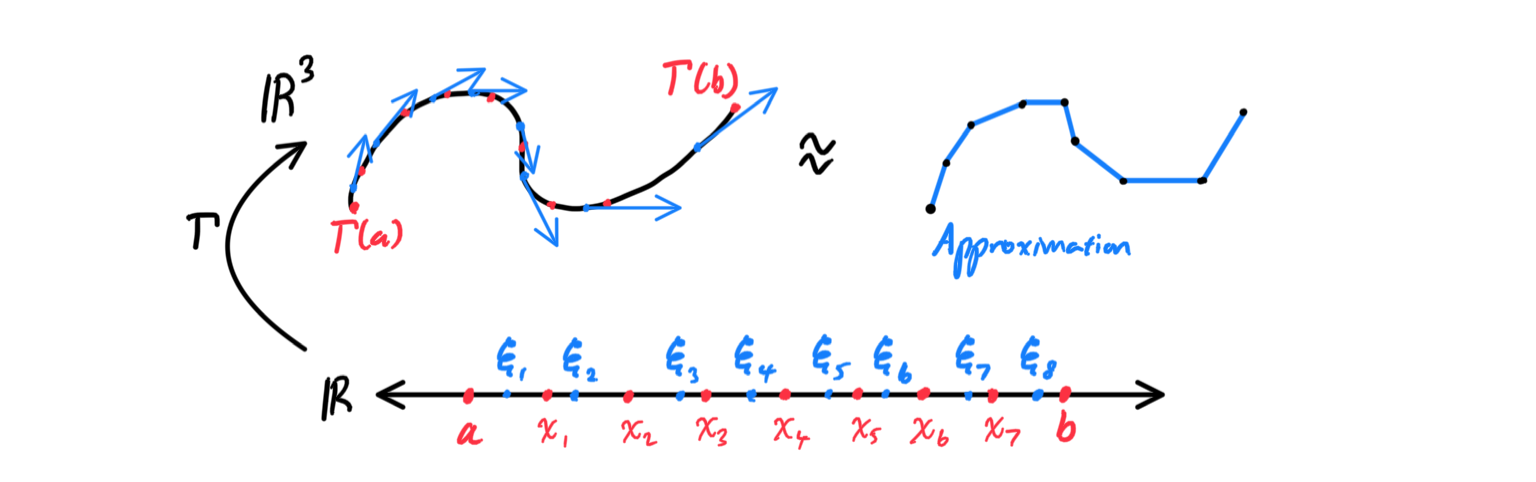
\includegraphics[scale=0.25]{img/Arc_Length_Integral.PNG}
      \end{center}
      An immediate result of this formula is the formula for the length of a graph of a function $f: [a, b] \longrightarrow \mathbb{R}$ in $\mathbb{R}^2$, by looking at the paramaterization $t \mapsto \Gamma(t) = \big(t, f(t)\big)$. 
      \[l[a,b] \equiv \int_a^b \sqrt{1 + (f^\prime (t))^2}\,dt\]
    \end{definition}

    The question on the effect of paramaterization on the integral now arises. 

    \begin{definition}[Admissible Change of Parameter]
      The path $\Tilde{\Gamma}: [\alpha, \beta] \longrightarrow \mathbb{R}^3$ is obtained from $\Gamma: [a, b] \longrightarrow \mathbb{R}^3$ by an \textbf{admissible change of parameter} if there exists a smooth mapping 
      \[T: [\alpha, \beta] \longrightarrow [a, b]\]
      such that $T(\alpha) = a, T(\beta) = b$, $T^\prime (\tau) > 0$ (that is, the reparamaterization $T$ is monotonic) on $[\alpha, \beta]$, and 
      \[\Tilde{\Gamma} = \Gamma \circ T\]
      The series of mappings can be represented with the following commutative diagram, where $I_{\alpha, \beta} = [\alpha, \beta] \subset \mathbb{R}$ and $I_{a, b} = [a, b] \subset \mathbb{R}$. 
      \[
        \begin{tikzcd}
          I_{\alpha, \beta} \arrow{r}{T} \arrow{rd}{\Tilde{\Gamma}}& I_{a, b} \arrow{d}{\Gamma}\\
           & \mathbb{R}^3
        \end{tikzcd}
      \]
      or with the more detailed visual below (Note that the points are labeled $0, 1, 2, 3, 4, 5$ do not represent numerical values, but rather the order in which the points are paramaterized. We can see from this ordering that $T$ is monotonic.)
      \begin{center}
          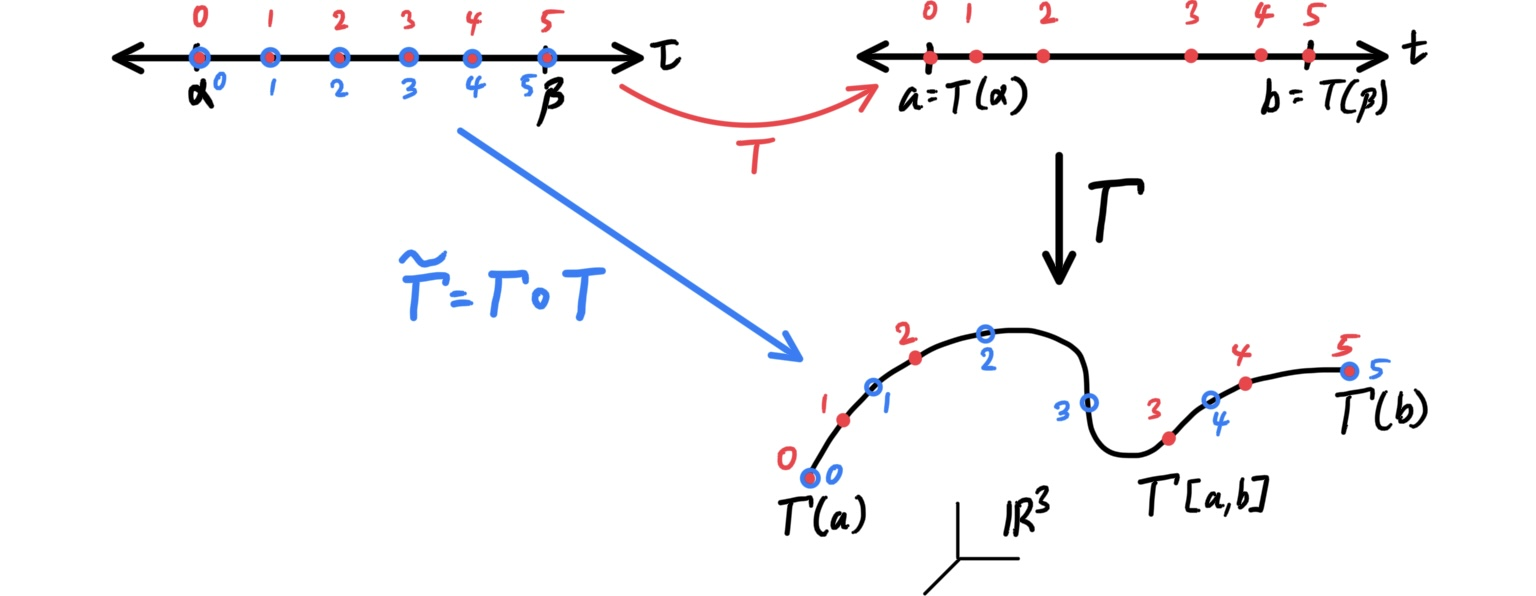
\includegraphics[scale=0.25]{img/Admissible_Change_of_Parameter.jpg}
      \end{center}
    \end{definition}

    \begin{theorem}[Invariance of Arclength Integral under Admissible Change of Parameters]
    If a smooth path $\Tilde{\Gamma}: [\alpha, \beta] \longrightarrow \mathbb{R}^3$ is obtained from a smooth path $\Gamma: [a, b] \longrightarrow \mathbb{R}^3$ by an admissible change of parameter, then the lengths of the two paths are equal. That is, a
    \[\int_a^b |\Gamma^\prime (t) |\,dt = \int_\alpha^\beta |\Tilde{\Gamma}^\prime (t)|\,dt \equiv \int_\alpha^\beta |(\Gamma \circ T)^\prime (t)|\,dt\]
    \end{theorem}

  \subsection{Improper Integrals}

    Due to some limitations of the Riemann integral, we cannot integrate over "singularities" where either the interval or the function is unbounded. We develop the tools of improper integration to deal with this problem; there are two types of improper integrals. 

    \begin{definition}[Improper Integral of Unbounded Interval]
      Suppose the function $x \mapsto f(x)$ is defined on the interval $[a, +\infty)$ and is integrable on every closed interval $[a, b]$ contained in that interval. Then, we call the following term
      \[\int_a^{+\infty} f(x)\,dx \equiv \lim_{b \rightarrow + \infty} \int_a^b f(x)\,dx\]
      the \textbf{improper Riemann integral of $f$ over the interval $[a, +\infty)$} and 
      \[\int_{-\infty}^b f(x)\,dx \equiv \lim_{a \rightarrow -\infty} \int_a^b f(x)\,dx \]
      the \textbf{improper Riemann integral of $f$ over the interval $(-\infty, b]$}.If the limit exists, then we say that the integral \textbf{converges} and \textbf{diverges} otherwise. 
    \end{definition}

    \begin{definition}[Improper Integral of Unbounded Function]
      Suppose the function $x \mapsto f(x)$ is defined on the interval $[a, B)$ and integrable on any closed interval $[a, b] \subset [a, B)$. Then, we call the following term
      \[\int_a^B f(x)\,dx \equiv \lim_{b \rightarrow B^-} \int_a^b f(x)\,dx\]
      the \textbf{improper Riemann integral of $f$ over interval $[a, B)$} and
      \[\int_A^b f(x)\,dx \equiv \lim_{a \rightarrow A^+} \int_a^b f(x)\,dx\]
      the \textbf{improper Riemann integral of $f$ over interval $(A,b]$}.
    \end{definition}

    For cohesiveness, we can combine these two definitions of improper integrals into the following one. 

    \begin{definition}[Improper Integrals]
      Let $[a, \omega)$ be a finite or infinite interval and $x \mapsto f(x)$ a function defined on that interval and integrable over every closed interval $[a, b] \subset [a, \omega)$. Then, by definition
      \[\int_a^\omega f(x)\,dx \equiv \lim_{b \rightarrow \omega} \int_a^b f(x)\,dx\]
      if this limit exists as $b \rightarrow \omega, b \in [a, \omega)$. Similarly, given the finite or infinite interval $(\omega, b]$ with $f$ integrable over every closed interval $[a, b] \subset (\omega, b]$, we have
      \[\int_\omega^b f(x)\,dx \equiv \lim_{a \rightarrow \omega} \int_a^b f(x)\,dx\]
      Note that if $\omega \in \mathbb{R}$ and $f \in \mathcal{R}[a, \omega]$, the improper integral is equivalent to the regular Riemann integral. 
      \[\int_a^\omega f(x) = \lim_{b\rightarrow \omega} \int_a^b f(x)\,dx\]
    \end{definition}

    \begin{lemma}[Properties of the Improper Integral]
      Suppose $f, g$ are functions defined on interval $[a, \omega)$ (without loss of generality, we let $\omega$ be the upper limit of integration) and integrable on every closed interval $[a, b] \subset [a, \omega)$. Suppose the improper integrals 
      \[\int_a^\omega f(x)\,dx \text{ and } \int_a^\omega g(x)\,dx\]
      are well-defined. 
      \begin{enumerate}
        \item For any $\lambda_1, \lambda_2 \in \mathbb{R}$ the function $(\lambda_1 f + \lambda_2 g)(x)$ is integrable in the improper sense on $[a, \omega)$ and
        \[\int_a^\omega (\lambda_1 f + \lambda_2 g)(x)\,dx = \lambda_1 \int_a^\omega f(x)\,dx + \lambda_2 \int_a^\omega g(x)\,dx\]
        \item For any $c \in [a, \omega)$, 
        \[\int_a^\omega f(x)\,dx = \int_a^c f(x)\,dx + \int_c^\omega f(x)\,dx\]
        \item If $\varphi: [\alpha, \gamma) \longrightarrow [a, \omega)$ is a smooth strictly monotonic mapping with $\varphi(\alpha) = a$ and $\varphi(\beta) \rightarrow \omega$ as $\beta \rightarrow \gamma^-$, then the improper integral of the function $t \mapsto (f \circ \varphi)(t) \varphi^\prime (t)$ over $[\alpha, \gamma)$ exists and 
        \[\int_a^\omega f(x)\,dx = \int_\alpha^\gamma (f \circ \varphi)(t) \varphi^\prime (t)\,dt\]
      \end{enumerate}
    \end{lemma}

    \subsubsection{Convergence of an Improper Integral}

      Note that by definition, an improper integral 
      \[\int_a^\omega f(x)\,dx \equiv \lim_{b \rightarrow \omega} \int_a^b f(x) \,dx\]
      is a limit of the function 
      \[\mathcal{F}(b) \equiv \int_a^b f(x)\,dx\]
      as $b \rightarrow \omega$. This means that we can use the Cauchy criterion to determine the convergence of this limit, and hence, existence of this improper integral. 

      \begin{theorem}[Cauchy Criterion for Convergence of an Improper Integral]
      If the function $x \mapsto f(x)$ is defined on the interval $[a, \omega)$ and integrable on every closed interval $[a, b] \subset [a, \omega)$, then the integral 
      \[\int_a^\omega f(x)\,dx\]
      converges if and only if for every $\epsilon > 0$ there exists $B \in [a, \omega)$ such that the relation
      \[\Bigg| \int_{b_1}^{b_2} f(x)\,dx \bigg| < \epsilon\]
      holds for any $b_1, b_2 \in [a, \omega)$ satisfying $B < b_1$ and $B < b_2$. 
      \end{theorem}
      \begin{proof}
      We have
      \[\int_{b_1}^{b_2} f(x)\,dx = \int_a^{b_2} f(x)\,dx - \int_a^{b_1} f(x)\,dx = \mathcal{F}(b_2) - \mathcal{F}(b_1)\]
      and therefore the condition is simply the Cauchy criterion for the existence of a limit for the function $\mathcal{F}(b)$ as $b \rightarrow \omega$. 
      \end{proof}

      \begin{definition}[Absolute Convergence of an Improper Integral]
        The improper integral 
        \[\int_a^\omega f(x)\,dx\]
        \textbf{converges absolutely} if the integral
        \[\int_a^\omega |f|(x)\,dx\]
        converges. Clearly, the inequality
        \[\Bigg| \int_{b_1}^{b_2} f(x)\,dx \Bigg| \leq \Bigg| \int_{b_1}^{b_2} |f|(x)\,dx \Bigg|\]
        implies that if an improper integral converges absolutely, then it converges. 
      \end{definition}

      This study of absolute convergence reduces to the study of convergence of integrals of nonnegative functions. The following lemma is useful in determining convergence of such functions. 

      \begin{lemma}
        Let there be a function $f$ defined on interval $[a, \omega)$ that is also integrable over every closed interval $[a, b] \subset [a, \omega)$. If $f(x) \geq 0$ on $[a, \omega)$, then the improper integral 
        \[\int_a^\omega f(x)\,dx\]
        exists if and only if the function 
        \[\mathcal{F}(b) \equiv \int_a^b f(x)\,dx\]
        is bounded on $[a, \omega)$. 
      \end{lemma}
      \begin{proof}
      It is clear that 
      \[\int_a^\omega f(x)\,dx = \lim_{b \rightarrow \omega} \mathcal{F}(b)\]
      If $f(x)\geq 0$, then the function $\mathcal{F}(b)$ is nondecreasing on $[a, \omega)$ and therefore has a limit as $b \rightarrow \omega$ only if it is bounded (since every monotonically increasing sequence that is bounded always converges). 
      \end{proof}

      This leads to the familiar integral test for convergence of a series. 

      \begin{theorem}[Integral Test for Convergence of a Series]
      If the function $x \mapsto f(x)$ is defined on the interval $[1, +\infty)$, nonnegative, nonincreasing, and integrable on each closed interval $[1, b] \subset [1, +\infty)$, then the series 
      \[\sum_{n=1}^\infty f(n) = f(1) + f(2) + \ldots\]
      and the integral 
      \[\int_a^{+\infty} f(x)\,dx\]
      either both converge or both diverge. 
      \end{theorem}

      We can use the comparison test analogue to determine convergence of improper integrals. 

      \begin{theorem}[Comparison Test for Convergence of Improper Integrals]
      Suppose the functions $f(x), g(x)$ are defined on the interval $[a, \omega)$ and integrable on any closed interval $[a, b] \subset [a, \omega)$. If 
      \[0 \leq f(x) \leq g(x)\]
      on $[a, \omega)$, then 
      \[\int_a^\omega g(x)\,dx \text{ converges} \implies \int_a^\omega f(x)\,dx \text{ converges}\]
      and the inequality 
      \[\int_a^\omega f(x)\,dx \leq \int_a^\omega g(x)\,dx\]
      holds. Also, 
      \[\int_a^\omega f(x)\,dx \text{ diverges} \implies \int_a^\omega g(x)\,dx \text{ diverges}\]
      \end{theorem}
    
    \subsubsection{Improper Integrals with Multiple Singularities}

      \begin{definition}[Improper Integral with Both Limits as Singularities]
        Given singularities $\omega_1, \omega_2$, the improper integral is defined
        \[\int_{\omega_1}^{\omega_2} f(x)\,dx \equiv \int_{\omega_1}^c f(x)\,dx + \int_c^{\omega_2} f(x)\,dx\]
        where $c$ is an arbitrary point in $(\omega_1, \omega_2)$. 
      \end{definition}

    \begin{example}[Gaussian Integral]
    The integral 
    \[\int_{-\infty}^{+\infty} e^{-x^2}\,dx = \sqrt{\pi}\]
    \end{example}


\section{Convergence} 

  \begin{definition}[Convergence in Measure]
    Let $(f_n)$ be a sequence of measurable and finite\footnote{We add finite condition since we avoid dealing with $+\infty - \infty$.} a.e. \textbf{$f_n \to f$ in measure} if for every $\eta > 0$, 
    \begin{equation}
      \lim_{n \to \infty} m \big( \{x \mid |f_n (x) - f(x)|  > \eta \}\big) = 0
    \end{equation}
    Colloquially, the set over which $f_n$ and $f$ differ too much is small. 
  \end{definition}

  So we have 3 types of convergence: uniform convergence, a.e. convergence, and now convergence in measure. Now we want to relate this convergence to the ones we already have. 

  \begin{theorem}
    Suppose $E$ is measurable, $m(E) < +\infty$, and $f_n \to f$ a.e. in $E$ (assume $f_n$ all measurable). Then , $f_n \to f$ in measure. 
  \end{theorem}
  \begin{proof}
    Observe that if $f_n \to f$ uniformly, then it converges in measure, because given some $\eta > 0$, $\exists N$ s.t. 
    \begin{equation}
      \{ x \mid |f_n (x) - f(x) | > \eta \} = \emptyset
    \end{equation}
    by definition. It doesn't go to $0$; it is $0$. You can guess why we started with this, because now we can directly use Egorov's theorem. Fix any $\epsilon > 0$. Find $E_0 \subset E$ s.t. $m (E \setminus E_0) < \epsilon$, and $f_n \to f$ uniformly on $E_0$. It follows that for all $\eta > 0$, 
    \begin{equation}
      m(\{x \mid |f_n (x) - f(x)| > \eta\}) \leq \epsilon 
    \end{equation}
    for all $n \geq N(\eta)$. Since this is true for every $\epsilon > 0$, so this implies
    \begin{equation}
      \lim_{n \to \infty} m(\{ x \mid |f_n (x) - f(x)| > \eta\}) = 0
    \end{equation} 
    for every $\eta > 0$. 
  \end{proof}

  A few remarks. First, if the measure of $E$ is infinite, this need not be true. Consider $f_n (x) = \chi_{[n, n+1]} (x)$. Then, this converges to $0$ pointwise, but it does not converge to $0$ in measure. There is always a measure $1$ set where $f$ is $1$. Where the proof breaks down is in Egorov's theorem, since it does not work when $m(E) = +\infty$. 

  The second remark is that the converse is not true. Consider $[0, 1]$ and the sequence of functions 
  \begin{equation}
    \chi_{[0, 1/2]}, \chi_{[1/2, 1]}, \chi_{[0, 1/4]}, \chi_{[1/4, 1/2]}, \chi_{[1/2, 3/4]}, \ldots 
  \end{equation}
  Then $f_n \to 0$ in measure since the size shrinks at the rate of $2^{-n}$. However, it doesn't converge a.e. since for any point $x \in [0, 1]$, the function will be $1$ eventually as we hit the subinterval containing $x$, like ``waves.'' So $f_n(x)$ diverges for all $x \in [0, 1]$. So indeed, convergence in measure is the weakest type of convergence. 

  Here is a sort-of converse. 

  \begin{theorem}[Riesz]
    Suppose $f_n \to f$ in measure. Then, there exists a subsequence $f_{n_k} \to f$ a.e. 
  \end{theorem}
  \begin{proof}
    For every $k$, find $n_k$ s.t. for all $n \geq n_k$,
    \begin{equation}
      m(\underbrace{\{x \mid |f_n(x) - f(x)| > 1/k\}}_{E_k}) < 2^{-k}
    \end{equation}
    Then, 
    \begin{equation}
      \sum_{k=1}^\infty m(E_k) < +\infty
    \end{equation}
    By Borel-Cantelli, the set of all $x$'s that are in infinitely many $E_k$ have measure $0$. So, almost everywhere, $x$ is only in a finite number of $E_k$. So for a.e., $x$, there exists $N(x)$ s.t. $x \not\in E_k$ for all $k \geq N(x)$. This means 
    \begin{equation}
      | f_{n_k} (x) - f(x)| < 1/k 
    \end{equation}
    for all $k \geq N(x)$. Therefore, $f_{n_k} (x) \to f(x)$ for a.e. $x$. 
  \end{proof}

  In the example above, we can just skip the functions that evaluate $x$ to $1$.  

  Practically, proving convergence in measure is still pretty good since we can pass in a subsequence that converges a.e. Here is a corollary. 

  \begin{corollary}
    Let $f_n \geq 0$, integrable on $E$. Then, 
    \begin{equation}
      \lim_{n \to +\infty} \int_E f_n \,dx = 0  \iff f_n \to 0 \text{ in measure}
    \end{equation}
    $f_n$ are tight and uniformly integrable. 
  \end{corollary}
  \begin{proof}
    We prove bidirectionally. 
    \begin{enumerate}
      \item $(\rightarrow)$. Tight, uniformly integrable is true be definition. Also, $f_n \to 0$ in measure by Chebyshev. 
        \begin{equation}
          m(\{x \mid f_n (x) > \eta\}) \leq \frac{1}{\eta} \int_E f_n \,dx 
        \end{equation}
      \item $(\leftarrow)$ For the opposite, we use the previous theorem. Find $f_{n_k}$ s.t. that it converges to $0$ a.e., and then use Vitali's convergence theorem. 
    \end{enumerate}
  \end{proof}

  In general, if $f_n \to 0$ in measure, it doesn't mean that the integral will go to $0$ since you can take larger and larger bumps. So we need extra assumptions. 

  \begin{lemma} 
    Suppose $f$ is bounded, and there exists measurable sequences of functions $\phi_n, \psi_n$ s.t. 
    \begin{equation}
      \psi_n (x) \leq f(x) \leq \psi_n(x) \quad \forall x \in E
    \end{equation}
    and 
    \begin{equation}
      \lim_{n \to +\infty} \int_E (\psi_n - \phi_n) = 0
    \end{equation}
    Then, there exists $\Tilde{phi}_n \to f$ and $\Tilde{psi}_n \to f$ a.e. 
  \end{lemma}
  \begin{proof}
    Define 
    \begin{equation}
      \Tilde{\phi}_n (x) = \max\{\phi_1 (x) , \ldots, \phi_n (x) \}, \quad \Tilde{\psi}_n (x) = \min\{\psi_1 (x) , \ldots, \psi_n (x) \}
    \end{equation}
    We still have $\Tilde{\phi}_n (x) \leq f(x) \leq \Tilde{\phi}_n (x)$ for all $n$ and for all $x$. Also, $\Tilde{\phi}_n (x)$ is increasing, $\Tilde{\psi}_n (x)$ is decreasing. Now define 
    \begin{equation}
      \phi^\ast (x) \coloneqq \lim_{n \to \infty} \Tilde{\phi}_n (x), \qquad \psi^\ast (x) \coloneqq \lim_{n \to \infty} \Tilde{\psi}_n (x)
    \end{equation}
    Observe that 
    \begin{equation}
      \int (\Tilde{\psi}_n - \Tilde{\phi}_n) \leq \int (\psi_n - \phi_n) \implies \int (\Tilde{\psi}_n - \Tilde{\phi}_n) \to 0 \text{ as } n \to \infty 
    \end{equation}
    Also, 
    \begin{equation}
      \int (\underbrace{\psi^\ast (x) - \phi^\ast(x)}_{\geq 0}) \,dx \leq \int (\Tilde{\psi}^\ast - \Tilde{\phi}^\ast) 
    \end{equation}
    for all $n$. Therefore, 
    \begin{equation}
      \int (\psi^\ast (x) - \phi^\ast (x)) = 0 \implies \psi^\ast (x) = \phi^\ast (x) \text{ a.e.}
    \end{equation}
    And so $f(x)$, which is sandwiched between $\psi^\ast$ and $\phi^\ast$, must be equal a.e. We didn't assume that $f$ was measurable, but these $\psi_n, \phi_n$ is measurable by assumption. 
  \end{proof}

  Now, we can prove this master theorem. 

  \begin{theorem}[Characterization of Lebesgue Integrability]
    Let $f$ be bounded on measurable set $E$ of finite measure. Then $f$ is Lebesgue integrable iff $f$ is measurable. 
  \end{theorem}
  \begin{proof}
    The backward implication is true in general. We want to show that $f$ is measurable. Recall that for bounded functions, we defined Lebesgue integrals with $\underline{L}f$ and $\overline{L}f$. Therefore, we can find simple $\phi_n, \psi_n$ s.t. $\phi_n \leq f \leq \psi_n$, and $\int \psi_n - \int \phi_n \leq 1/n$. Now we are exactly in the setting of the lemma, and so by the lemma, we can find measurable $\Tilde{\psi}_n (x) \to f$ a.e. (in fact, $\Tilde{\psi}$ will be simple). Since the limit of measurable functions is measurable, $f$ is measurable.
  \end{proof}

  This is a very reasonable criterion, and you can't really hope for more then Lebesgue measurability. This following theorem on Riemmann integrability is much more restrictive, while for above, measurable functions can be very wild. 

  \begin{theorem}[Characterization of Riemann Integrability]
    $f$ is Riemann integrable on $[a, b]$ if the set of its discontinuities has measure $0$. 
  \end{theorem}
  \begin{proof}
    Not stated. In book. 
  \end{proof}


  Oct 8. Now we will build the theory of differentiation on monotone functions. 

  \begin{definition}[]
    Given a set $E$, a collection $\mathcal{F}$ \textbf{covers $E$ in Vitali sense} if $\forall x \in E, \forall \epsilon > 0$, there exists $I \in \mathcal{F}$ s.t. $x \in I$, $\ell(I) < \epsilon$. 
  \end{definition}

  Note that we don't assume that $E$ is measurable. It is easy to see that a Vitali set can be uncountable (all subintervals of $[0, 1]$) and even countable (all subintervals with rational endpoints). Nevertheless, we can still select a finite set of intervals that almost covers $E$. 

  \begin{lemma}[Vitali Covering Lemma]
    Suppose $m^\ast (E) < +\infty$ and $\mathcal{F}$ covers $E$ in Vitali sense. Then, $\forall \epsilon > 0$, $\exists$ a disjoint finite collection $I_1, I_2, \ldots, I_n$ of intervals from $\mathcal{F}$ s.t. 
    \begin{equation}
      m^\ast \bigg( E \setminus \bigcup_{k=1}^n I_k \bigg) < \epsilon
    \end{equation}
  \end{lemma}
  \begin{proof}
    Since $m^\ast (E) < +\infty$, by definition $\exists$ open $O$ s.t. $E \subset O$, $m(O) < +\infty$. WLOG we can assume that all intervals in $\mathcal{F}$ lie in $O$.\footnote{We can just discard any interval that it not Vitali in $O$ and keep only those intervals in $O$ such that it would still be in a Vitali cover. Indeed, we can discard all $I \subset \mathcal{F}$ s.t. $I \not\subset O$. Given $x \in E, x \in O$, so $d(x, O^c) > 0$ for all $\epsilon > 0$, $\exists I \in F$ s.t. $\ell(I) < \epsilon$, $x \in I, I \subset O$ (just take $\ell(I), < \min(\epsilon, d(x, O^c))$). So even remaining intervals cover $E$ in Vitali sense. }

    Note two things. 
    \begin{enumerate}
      \item If $I_1, I_2, \ldots, I_n$ are disjoint and belong to $O$, then $\sum_{k=1}^n \ell(I_k) < +\infty$ since it is less than the measure of $O$ which is finite. 

      \item Second, if we have finite collection $\{I_k\}_{k=1}^n \in \mathcal{F}$ , define 
      \begin{equation}
        \mathcal{F}_n \coloneqq \{I \in \mathcal{F} \mid I \cap \bigcup_{k=1}^n I_k = \emptyset \}
      \end{equation}
      Then every $x \in E \setminus \bigcup_{k=1}^n I_k$ lies in some $I \in \mathcal{F}_n$. 
    \end{enumerate}

    The ideal is to define $I_1, \ldots, I_n \in \mathcal{F}$ s.t. they are disjiont and 
    \begin{equation}
      E \setminus \bigcup_{k=1}^n I_k \subset \bigcup_{k=n+1}^\infty 5 I_k \quad \forall n \label{inclusion}
    \end{equation}
    where $5I$ means that we keep the center of the interval fixed and scale it up by 5 times. If we do that, then $\forall \epsilon > 0$, find $n$ s.t. $\sum_{k=n+1}^\infty \ell(I_k) < \epsilon / 5$. Take $I_1, \ldots, I_n$ as our intervals 
    \begin{equation}
      m^\ast \bigg( E \setminus \bigcup_{k=1}^n I_k \bigg) \leq \sum_{k=n+1}^\infty \ell(5 I_k) < \epsilon
    \end{equation}
    So it remains to select these intervals $I_1, \ldots, I_n$. We will do this inductively. 
    \begin{enumerate}
      \item $I_1$ be any interval in $\mathcal{F}$ s.t. 
      \begin{equation}
        \ell(I_1) \geq \frac{1}{2} \sup_{I \in \mathcal{F}} \ell(I) 
      \end{equation}

      \item Once $I_1, \ldots, I_n$ have been selected, we select $I_{n+1}$ from $\mathcal{F}_n$ s.t. 
      \begin{equation}
        \ell(I_{n+1}) \geq \frac{1}{2} \sup_{I \in \mathcal{F}_n} \ell(I)
      \end{equation}
      So these intervals are clearly disjoint from the ones that we have selected earlier. So it remains to show \ref{inclusion}. Suppose $x \in E \setminus \cup_{k=1}^n I_k$. Then, $\exists I \in \mathcal{F}_n$ s.t. $x \in I$. 
    \end{enumerate}
    Suppose $I \in \mathcal{F}_m$ for all $m \geq n$. This is impossible since by construction, $\ell(I_m) \geq \frac{1}{2} \ell(I)$. This contradicts $\sum \ell(I_m)$ is finite. Therefore, $\exists m$ s.t. $I \in \mathcal{F}_{m-1}$ but $I \not\in \mathcal{F}_m$. This implies that $I \cap I_m \neq \empty$ (while the intersection with the previous ones were empty). But then, $I \subset 5 I_m$, since $\ell(I_m) \geq \frac{1}{2} \ell(I)$.\footnote{The $5$ is needed since we have $1/2$. So we are taking the midpoint $3/4$ of the interval $[1/2, 1] \subset [0, 1]$, which should be blown up by $5$. } 
  \end{proof}

  This may be a heavy proof, but this lemma seems to be very convenient. 

  \begin{definition}[Derivative]
    Given any $f$ and $x$ in the interior of its domain, we can define the \textbf{upper and lower derivative} as
    \begin{equation}
      \overline{D} f(x) \coloneqq \lim_{h \to 0} \sup_{0 < |t| < h} \frac{f(x + t) - f(x)}{t}, \qquad \underline{D} f(x) \coloneqq \lim_{h \to 0} \inf_{0 < |t| < h} \frac{f(x + t) - f(x)}{t} 
    \end{equation}
    If they are equal, then we can define the \textbf{derivative} as either one, and we say $f$ is \textbf{differentiable} at $x$. 
  \end{definition}

  Note that as $h$ goes to $0$, the first is nondecreasing and the second is nonincreasing, and clearly 
  \begin{equation}
    \underline{D} f(x) \leq \overline{D} f(x)
  \end{equation}

  \begin{lemma} 
    Suppose $f$ is increasing on $[a, b]$. Then $\forall \alpha > 0$, then, 
    \begin{equation}
      m^\ast \{ x \mid \overline{D} f(x) \geq \alpha \} \leq \frac{1}{\alpha} \big( f(b) - f(a) \big)
    \end{equation}
    and 
    \begin{equation}
      m^\ast \{ x \mid \overline{D} f(x) = \infty\} = 0
    \end{equation}
  \end{lemma}
  \begin{proof}
    Fix $\alpha > 0$, define $E_\alpha = \{ x \mid \overline{D} f(x) \geq \alpha\}$. Take any $\alpha^\prime < \alpha$, any $\epsilon > 0$. Consider all intervals $[c, d] \subset [a, b]$ s.t. $f(d) - f(c) > \alpha^\prime (d - c)$. This collection covers $E_\alpha$ in Vitali sense. Since no matter how small $h$ is, we can find $t$ so that this ratio term is bigger than $\alpha^\prime$. 

    Now, we can use the covering lemma to find a finite disjoint collection $\{[c_k, d_k]\}_{k=1}^n$ s.t. $m^\ast ( E \setminus \cup_{k=1}^n [c_k, d_k]) < \epsilon$. Then, 
    \begin{equation}
      m^\ast (E) \leq \sum_{k=1}^n (d_k - c_k) + \epsilon 
    \end{equation}
    by subadditivity of outer measure. Using the inequality, 
    \begin{equation}
      \leq \frac{1}{\alpha^\prime} \sum_{k=1}^n \big( f(d_k) - f(c_k) \big) + \epsilon
    \end{equation}
    But $f$ is monotone, so 
    \begin{equation}
      \leq \frac{1}{\alpha^\prime} \big( f(b) - f(a) \big) + \epsilon
    \end{equation}
    This is true for all $\alpha^\prime < \alpha$ for all $\epsilon > 0$, proving the first claim. The second part follows since it is an intersection of all sets for $\alpha = n$ for all $n \in \mathbb{N}$, which go to $0$. 
  \end{proof}

  Since we are using outer measure, we don't have to worry nor rely on about measurability. Also, there can be uncountable set at which $f$ is infinite, but it just guarantees outer measure $0$.  
  
  \begin{theorem}[Lebesgue]
    Suppose $f$ is increasing on $(a, b)$. Then, it is differentiable a.e. on $(a, b)$. 
  \end{theorem}
  \begin{proof}
    WLOG, $(a, b)$ is bounded.\footnote{Otherwise, we can always split it into a countable union of bounded intervals. } Consider the countable family of sets 
    \begin{equation}
      E_{\alpha, \beta} = \{x \mid \overline{D} f (x) > \alpha > \beta > \underline{D}f(x), \alpha, \beta \in \mathbb{Q} \}
    \end{equation}
    Note that if the derivatives aren't equal, we can always squeeze 2 rationals in, so 
    \begin{equation}
      \{x \mid \overline{D} f(x) > \underline{D} f(x) \} \subset \bigcup_{\alpha, \beta \in \mathbb{Q}} E_{\alpha, \beta}
    \end{equation}
    We want to prove that $m^\ast (E_{\alpha, \beta}) = 0 \quad \forall \alpha, \beta$. Let's find $O$ open s.t. $E_{\alpha, \beta} \subset O$ and $m(O) < m^\ast (E) + \epsilon$, where we will denote $E = E_{\alpha, \beta}$. 

    Consider all intervals $[c, d] \subset O$ s.t. $f(d) - f(c) < \beta (d - c)$. Since we know $\underline{D} f(x) < \beta$, these intervals cover $E$ in Vitali sense. So you find a disjoint subcollections $[c_k, d_k]$ for $k = 1, \ldots, n$ s.t. 
    \begin{equation}
      m^\ast \bigg( E \setminus \bigcup_{k=1}^n [c_k, d_k] \bigg) < \epsilon 
    \end{equation}
    Observe that 
    \begin{align}
      \sum_{k=1}^n \big( f(d_k) - f(c_k) \big) & < \beta \sum_{k=1}^n (d_k - c_k) \\ 
                                               & \leq \beta \big( m^\ast (E) + \epsilon \big)
    \end{align}
    On the other hand, we can apply the previous lemma to $E \cap [c_k, d_k]$ to get 
    \begin{equation}
      m^\ast (E \cap [c_k, d_k]) \leq \frac{1}{\alpha} \big( f(d_k) - f(c_k) \big) 
    \end{equation}
    and so 
    \begin{align}
      m^\ast (E) & \leq \frac{1}{\alpha} \sum_{k=1}^n \big( f(d_k) - f(c_k) \big) + \epsilon \\ 
                 & \leq \frac{\beta}{\alpha} \big( m^\ast(E) + \epsilon) + \epsilon, \quad \forall \epsilon > 0 
    \end{align}
    So, $m^\ast(E) \leq \frac{\beta}{\alpha} m^\ast (E)$, where $\frac{\beta}{\alpha} < 1$. Therefore $m^\ast (E) = 0$. 
  \end{proof}

  But being differentiable doesn't imply that fundamental theorem of calculus holds. So integrating the derivative won't get you back these functions (think of step functions). So we will have to specify a class of functions such that this holds. 

  \begin{corollary}
    Suppose $f$ is increasing on $[a, b]$. Then $f^\prime$ is integrable, and 
    \begin{equation}
      \int_a^b f^\prime \leq f(b) - f(a)
    \end{equation}
  \end{corollary}
  \begin{proof}
    Define 
    \begin{equation}
      D_n f(x) = \frac{f(x + 1/n) - f(x)}{1/n}
    \end{equation}
    by Lebesgue theorem, $D_n f \to f^\prime$ a.e. By Fatau, 
    \begin{equation}
      \int_a^b \leq \liminf \int_a^b D_n f = 
    \end{equation}
    where 
    \begin{align}
      \int_a^b D_n f & = n \int_{a + 1/n}^{b + 1/n} f(x) - n \int_a^b f(x) \\
                     & = n \bigg( \int_b^{b + 1/n} f(b) - \int_a^{a + 1/n} f(x) \bigg) \\ 
                     & \leq f(b) - f(a)
    \end{align}
    Here we extended $f(x)$ by $f(b)$ for $x \in [b, b + \frac{1}{n}]$. 
  \end{proof}

  \begin{example}
    If $f$ is not monotone but continuous, $f^\prime$ doesn't have to be integrable. Consider 
    \begin{equation}
      f(x) = x^2 \sin \Big( \frac{1}{x^2} \Big)
    \end{equation}
    on $[0, 1]$. Then 
    \begin{equation}
      f^\prime (x) 2 x \sin \Big( \frac{1}{x^2} \Big) - \frac{2}{x} \cos \Big( \frac{1}{x^2} \Big)
    \end{equation}
  \end{example}

\section{Conditional Expectation}

  Conditional expectation is extremely important, especially in the context of stochastic processes, which is talked about in more detail in another set of notes. 

  First, note that when we talk about the probability of event $A$ happening, or equivalently, the probability of $\omega \in A$, we can write this as the expected value of the indicator function $A$. 
  \begin{equation}
    \mathbb{P}(A) = \mathbb{E}[1_A]
  \end{equation}
  This will come in handy later in connecting conditional probability and expectation. 

  Now conditional expectation is quite tricky to understand at first. We will start by defining it given a $\sigma$-algebra and then given a random variable. 

  \begin{definition}[Conditional Expectation]
    Given a probability space $(\Omega, \mathcal{F}, \mathbb{P})$, a sub-$\sigma$-algebra $\mathcal{G} \subset \mathcal{F}$, and an $\mathcal{F}$-measurable random variable $X$ (with $\mathbb{E}[X] < \infty$), the \textbf{conditional expectation of $X$ given $\mathcal{G}$} is defined to be the $\mathcal{G}$-measurable random variable $Y = \mathbb{E}[X \mid \mathcal{G}]$ satisfying 
    \begin{equation}
      \int_A X \,d\mathbb{P} = \int_A Y \,d \mathbb{P}
    \end{equation}
    or equivalently, 
    \begin{equation}
      \mathbb{E}[X \cdot 1_A] = \mathbb{E}[Y \cdot 1_A]
    \end{equation}
    for all $A \in \mathcal{G}$. Any $Y$ satisfying these two conditions is said to be a \textbf{version} of $\mathbb{E}[X \mid \mathcal{F}]$. The critical detail to note here is that the conditional expectation $Y$, has the same expected value as $X$ does, not over just the whole $\mathcal{G}$, but \textit{in every subset $G$ of $\mathcal{G}$}. 
  \end{definition}

  We state without proof that $\mathbb{E}[X \mid \mathcal{G}]$ exists and is almost surely unique. For now, we can interpret this as the best approximation of the $\mathcal{F}$-measurable $X$ with the $\mathcal{G}$-measurable $Y$. Here is a useful analogy. Say that we have some "fine" function $X$ defined on the interval $[0, 1]$ with a fine Borel $\sigma$-algebra $\mathcal{F}$. 
  \begin{enumerate}
    \item If we are given some sub-$\sigma$-algebra $\mathcal{G}$ composed of $\emptyset, [0, 0.5], (0.5, 1], [0, 1]$, then $Y$ would be the step function defined constantly on these intervals. 
    \item If we are given a finer sub-$\sigma$-algebra $\mathcal{H}$ generated by $[0, 0.25), [0.25, 0.5), [0.5, 0.75), [0.75, 1]$, then this would give a $\mathcal{H}$-measurable function that is a better approximation of $X$. 
  \end{enumerate}
  \begin{center}
    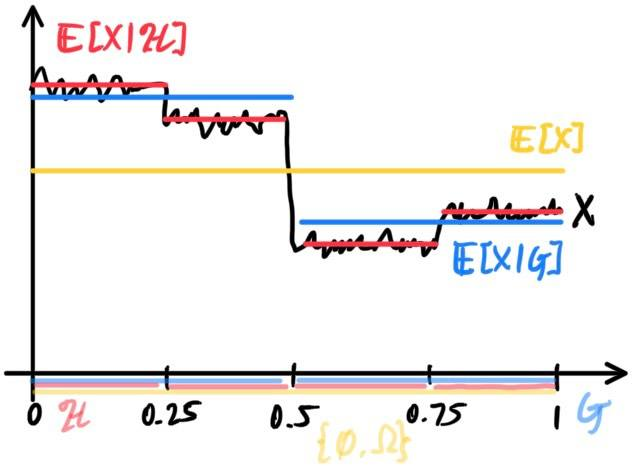
\includegraphics[scale=0.33]{img/function_approximation_conditional.jpg}
  \end{center}

  Therefore, we can see that if $\mathbb{E}[X \mid \mathcal{G}]$ is $\mathcal{F}$-measurable, then 
  \begin{equation}
    X = \mathbb{E}[X \mid \mathcal{G}]
  \end{equation}
  since its value coincides with $X$ for every event in $\mathcal{F}$. One way to think about it is that $\mathbb{E}[X \mid \mathcal{G}]$ is the conditional expectation of $X$ (which is "detailed" up to resolution $\sigma(\mathcal{G})$) taken with a camera of resolution $\mathcal{G}$. The finer (bigger) the $\sigma$-algebra is, the higher the resolution. 

\subsection{Properties of Conditional Expectation}

  \begin{theorem}[Tower Rule]
    The expectation of $X$ and its approximation always coincides. 
    \begin{equation}
      \mathbb{E}[X] = \mathbb{E}[\mathbb{E}[X \mid \mathcal{G}]]
    \end{equation}
  \end{theorem}

  \begin{lemma}
    Let $\mathbb{E}[|X|] , \mathbb{E}[|Y|] < \infty$. Then, 
    \begin{enumerate}
      \item Conditional expectation is linear
      \begin{equation}
        \mathbb{E}[a X + b Y \mid \mathcal{G}] = a \mathbb{E}[X \mid \mathcal{G}] + b \mathbb{E}[Y \mid \mathcal{G}]
      \end{equation}
      
      \item If $X \leq Y$, then 
      \begin{equation}
        \mathbb{E}[X \mid \mathcal{G}] \leq \mathbb{E}[Y \mid \mathcal{G}]
      \end{equation}
    \end{enumerate}
  \end{lemma}

  \begin{theorem}[Jensen's Inequality]
    If $\varphi$ is convex and $\mathbb{E}[|X|], \mathbb{E}[|\varphi(X)|] < \infty$, then 
    \begin{equation}
      \varphi(\mathbb{E}[X \mid \mathcal{G}]) \leq \mathbb{E}[\varphi(X) \mid \mathcal{G}]
    \end{equation}
  \end{theorem}

  \begin{theorem}
    Conditional expectation is a contraction in $L^p$, $p \geq 1$. 
  \end{theorem}

  \begin{theorem}
    If $X$ is $\mathcal{F}$-measurable and $\mathbb{E}[|Y|], \mathbb{E}[|XY|] < \infty$, then 
    \begin{equation}
      \mathbb{E}[XY \mid \mathcal{F}] = X \mathbb{E}[Y \mid \mathcal{F}]
    \end{equation}
  \end{theorem}

  \begin{theorem}
    Suppose $\mathbb{E}[X^2] < \infty$. Then, $\mathbb{E}[X \mid \mathcal{G}]$ is the $\mathcal{G}$-measurable function $Y$ that minimizes the mean squared error 
    \begin{equation}
      \mathbb{E}[ (X - Y)^2]
    \end{equation}
  \end{theorem}

  This gives a nice geometric interpretation of $\mathbb{E}[X \mid \mathcal{G}]$. Given that $X$ lives in the Hilbert space $L^2_\mathcal{F} (\Omega)$, $\mathbb{E}[X \mid \mathcal{G}]$ is the projection of $X$ onto the subspace $L^2_\mathcal{G} (\Omega)$. 
  \begin{center}
    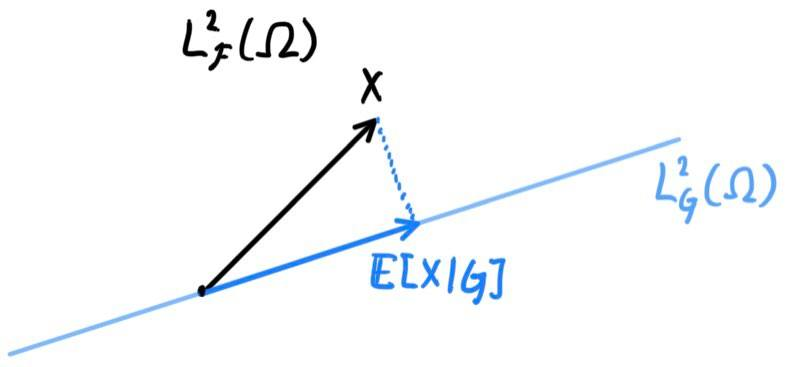
\includegraphics[scale=0.3]{img/Hilbert_Space_projection.jpg}
  \end{center}
  Therefore, we can change the way think about $\mathbb{E}[X]$. It is not just a value, but rather, we can think of it as our best prediction of $X$ given no information. Specifically, 
  \begin{equation}
    \mathbb{E}[X] = \mathbb{E}[X \mid \{\emptyset, \Omega\}]
  \end{equation}
  That is, letting $\mathcal{G}$ be the trivial $\sigma$-algebra, we must find the best approximation of $X$ that is $\mathcal{G}$-measurable. But any random variable that is $\mathcal{G}$-measurable must be constant, since if we take the preimage of any singleton set $\{x\} \in \mathcal{R}$, then it must be either $\emptyset$ ($X$ does not map to it) or $\Omega$ ($X$ maps all of $\Omega$ to it).

\subsection{Perfect Information vs No Information}

  Now let us state some properties on how certain $\sigma$-algebras can change the conditional expectation of certain random variables. 

  \begin{theorem}[Perfect Information]
    If $X$ is $\mathcal{G}$-measurable, then 
    \begin{equation}
      \mathbb{E}[X \mid \mathcal{G}] = X
    \end{equation}
    That is, the values of $X$ are defined on $\sigma(X) \subset \mathcal{F}$ and so has a detail level of $\sigma(X)$. But if we condition it on an even finer $\mathcal{G} \supset \sigma(X)$, then we are taking a picture of $X$ with something that has overly high resolution, and so our best approximation of $X$ is $X$ itself. Indeed, if $X$ lives in $L_\mathcal{G} (\Omega)$, then its projection onto $L_\mathcal{G} (\Omega)$ is $X$ itself. 
  \end{theorem}

  \begin{theorem}[Irrelevant Information]
    If $X$ is independent of $\mathcal{G}$, i.e. $\sigma(X)$ and $\mathcal{G}$ are independent $\sigma$-algebras, then 
    \begin{equation}
      \mathbb{E}[X \mid \mathcal{G}] = \mathbb{E}[X]
    \end{equation}
    That is, our best approximation of $X$ given information $\mathcal{G}$ is $\mathbb{E}[X]$ itself, i.e. if you don't know anything about $X$, then the best guess is the mean $\mathbb{E}[X]$. To see why, note that independence means that for all $A \in \mathcal{G}$ and $B \in \mathcal{R}$, 
    \begin{equation}
      \mathbb{P}(X^{-1} (B) \cap A) = \mathbb{P}(X^{-1}(B)) \cdot \mathbb{P}(A)
    \end{equation}
  \end{theorem}

  \begin{theorem}[Trivial Information]
    If $\mathcal{G} = \{\emptyset, \Omega\}$, then 
    \begin{equation}
      \mathbb{E}[X \mid \mathcal{G}] = \mathbb{E}[X]
    \end{equation}
    This makes sense since we're trying to measure $\sigma(X)$-measurable $X$ with the trivial $\mathcal{G}$, and the only function that is measurable w.r.t. the trivial $\sigma$-algebra is a constant function (since the preimage of every Borel set in $\mathcal{R}$ must be either $\Omega$ or $\emptyset$). This is the same as projecting $X$ to the line of constant functions in $L_\mathcal{F}(\Omega)$. 
  \end{theorem}

  \begin{theorem}
    If $\mathcal{F}_1 \subset \mathcal{F}_2$, then 
    \begin{enumerate}
      \item $\mathbb{E}[ \mathbb{E}[X \mid \mathcal{F}_1] \mid \mathcal{F}_2] = \mathbb{E}[X \mid \mathcal{F}_1]$. 
      \item $\mathbb{E}[ \mathbb{E}[X \mid \mathcal{F}_2] \mid \mathcal{F}_1] = \mathbb{E}[X \mid \mathcal{F}_1]$. 
    \end{enumerate}
    In other words, the smaller $\sigma$-algebra always wins. 
  \end{theorem}

  We can see this visually since in both cases, we are projecting $X$ onto $L^2_{\mathcal{F}_1} (\Omega)$ and onto $L^2_{\mathcal{F}_2} (\Omega)$, but either way, we end up in $L^2_{\mathcal{F}_1} (\Omega)$. Additionally, this is also consistent with our camera analogy, where $\mathbb{E}[X \mid \mathcal{G}]$ is like taking a picture of random variable $X$ with a camera of resolution $\mathcal{G}$. Conditional expectation is essentially an averaging/blurring operator. So, $\mathbb{E}[\mathbb{E}[X \mid \mathcal{G}] \mid \mathcal{H}]$ is like taking a picture of $X$ with resolution $\mathcal{H}$ and then with $\mathcal{G}$. The lower resolution would always win. 

\subsection{Computation of Conditional Expectation}

  \begin{definition}
    Given probability space $(\Omega, \mathcal{F}, \mathbb{P})$, the conditional expectation of $Y$ given $X$ is the random variable 
    \begin{equation}
      \mathbb{E}[X \mid Y] \coloneqq \mathbb{E}[X \mid \sigma(Y)]
    \end{equation}
    Note that since both $X$ and $Y$ are random variables, they are both $\mathcal{F}$-measurable. However, this doesn't mean that they may be $\mathcal{G}$-measurable for some sub-$\sigma$-algebra $\mathcal{G}$. So, as long as $\sigma(Y) \subset \sigma(X)$ (neither of which may be $\mathcal{F}$), we have some nontrivial approximation. 
  \end{definition}

  Now let's introduce a new way to think about expectation and conditional expectation in general. 
  \begin{enumerate}
    \item The first step is to think of $\mathbb{E}[X]$ not as a value $\mu$ but as the best estimate for the value of a random variable $X$ in the absence of any information. To minimize the squared error 
    \begin{equation}
      \mathbb{E}[ (X - e)^2] = \mathbb{E}[ X^2 - 2 e X + e^2] = \mathbb{E}[X^2] - 2 e \mathbb{E}[X] + e^2
    \end{equation}
    we differentiate with respect to $e$ to obtain $2e - 2 \mathbb{E}[X] = 0 \implies e = \mathbb{E}[X]$. For example, if I throw a fair die and you have to estimate its value $X$, according to the analysis above, your best bet is to guess $\mathbb{E}[X] = 3.5$ since $\Omega = \{1, 2, 3, 4, 5, 6\}$. On specific rolls of the die, this will be an over-estimate of an underestimate, but on the long run it minimizes the mean square error. 
    
    \item If we \textit{do} have additional information, then we use conditional expectation. Suppose that I tell you that $X$ is an even number. Then, I would guess that the possible values of $X$ are $\{2, 4, 6\}$, and so the our conditional expectation is $4$. Similarly, if I told you that $X$ is odd, then the conditional expectation is $3$. This additional information can be put into a random variable $Y: \Omega \rightarrow \mathbb{R}$ defined 
    \begin{equation}
      Y(\omega) = \begin{cases} 0 & \text{ if } \omega = 2, 4, 6 \\ 1 & \text{ if } \omega = 1, 3, 5 \end{cases}
    \end{equation}
    Then, we can say that $\mathbb{E}[X \mid Y = 0] = 4$ and $\mathbb{E}[X \mid Y = 1] = 3$. We can interpret this as the conditional expectation given the $\sigma$-algebra generated by these two sets $\{2, 4, 6\}$ and $\{1, 3, 5\}$. 
    
    \item Now, imagine that I roll the die and I tell you the parity of $X$. You should see that a single numerical response cannot cover both cases. You would respond $3$ if I tell you $X$ is odd ($Y = 1$) and $4$ if I tell you $X$ is even ($Y = 0$). A single numerical response is not enough because the particular piece of information I give you is \textit{itself random}. In fact, your response is necessarily a function of this particular piece of information, represented in our notation as 
    \begin{equation}
      g(Y) = \mathbb{E}[X \mid Y] = \begin{cases} 3 & \text{ if } Y = 1 \\ 4 & \text{ if } Y = 0 \end{cases}
    \end{equation}
    This is a function of $Y$, and it is consistent with our understanding of $\mathbb{E}[X \mid Y]$ as our "best estimate" of $X$ with random variable $Y$. 
    \begin{center}
      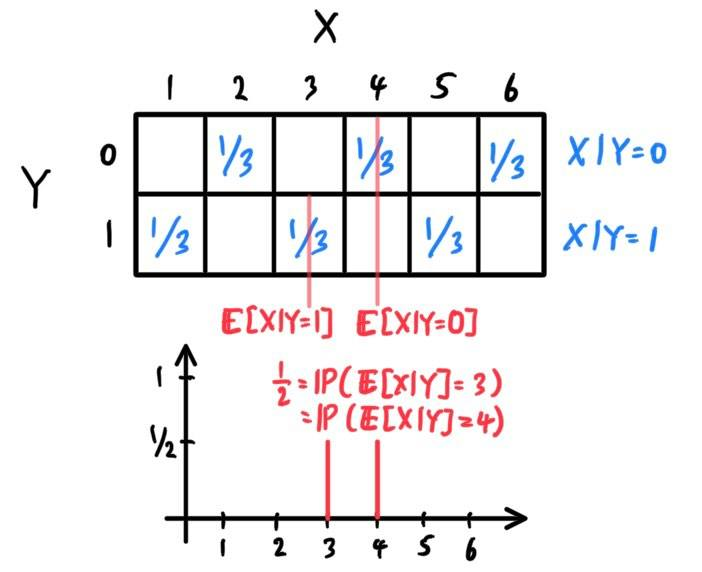
\includegraphics[scale=0.3]{img/conditional_expect_dice.jpg}
    \end{center}
  \end{enumerate}

  From the visual above, we can see that we take the joint distribution $X \times Y$, and for each value $Y = y$, we can estimate $X$ as $\mathbb{E}[X \mid Y = y]$. But now there is the additional uncertainty of what value $Y$ will take, which turns this value estimate $\mathbb{E}[X \mid Y = y]$ in a distribution $\mathbb{E}[X \mid Y]$. So, for the discrete case, 
  \begin{equation}
    \mathbb{P}\big( \mathbb{E}[X \mid Y] = \mathbb{E}[X \mid Y = y]) = \mathbb{P}(Y = y)
  \end{equation}

  Now we can talk about how to compute conditional expectation. In essence, the conditional expectation $\mathbb{E}[X \mid Y]$ is simply a function of a random variable $Y$ that is this best approximation. Given a joint random variable $(X, Y): \Omega \rightarrow \mathbb{R}^2$, we can fix a value of $Y = y$. Therefore, we are given the information that event $Y^{-1}(\{y\})$ happened, and so we can construct our conditional distribution $X \mid Y = y$, which defines a new probability measure. Taking the expectation of that gives us a number. 


  \begin{definition}[Discrete Conditional Expectation Given $Y = y$]
    Let $X, Y$ be discrete random variables, with joint random variable $(X, Y): \Omega \rightarrow \mathbb{R}^2$ and its joint PMF $p_{X, Y} (x, y)$. Recall that the conditional PMF is 
    \begin{equation}
      p_{X\mid Y}(x \mid y) \coloneqq \frac{p_{X, Y} (x, y)}{p_Y (y)}
    \end{equation}
    The \textbf{conditional expectation} of $X$ given $Y = y$ is 
    \begin{equation}
      \mathbb{E}[X \mid Y = y] = \sum_{x \in \mathcal{X}} x \, p_{X \mid Y} (x \mid y)
    \end{equation}
  \end{definition}

  \begin{definition}[Continuous Conditional Expectation Given $Y = y$]
    Let $X, Y$ be jointly continuous with joint PDF $f_{X, Y} (x, y)$. Recall that the conditional PDF is 
    \begin{equation}
      f_{X \mid Y} (x \mid y) \coloneqq \frac{f_{X, Y} (x, y)}{f_Y (y)}
    \end{equation}
    The \textbf{conditional expectation} of $X$ given $Y = y$ is 
    \begin{equation}
      \mathbb{E}[X \mid Y = y] = \int_{x \in \mathbb{R}} x \, f_{X \mid Y} (x \mid y) \, dx
    \end{equation}
    Again, we can set $\psi(y) \coloneqq \mathbb{E}[X \mid Y = y]$, which is a function of $y$ and therefore a random variable. 
  \end{definition}

  As a visual, we can take a "slice" of the joint distribution of some value of $Y$, look at the distribution of $X$ on this slice, and compute its expectation. That is, for every value of $Y = y$, there exists some (conditional) distribution of $X$ with PMF of $p_{X \mid Y} (x \mid y)$ or PDF of $f_{X \mid Y} (x \mid y)$. 
  \begin{center}
    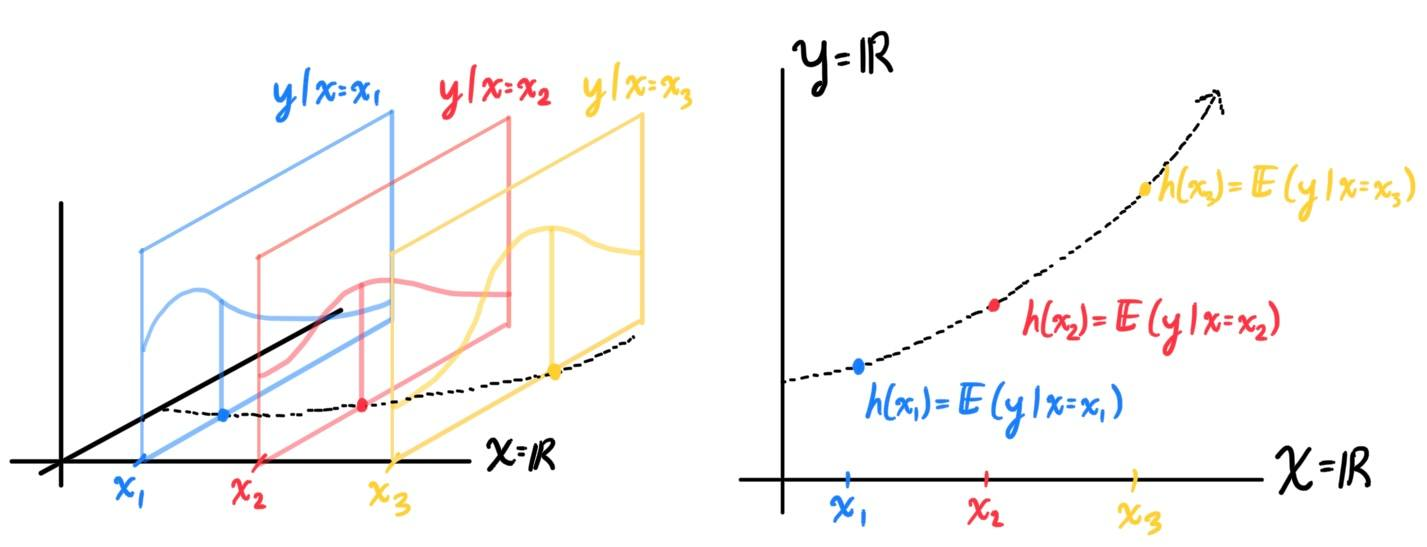
\includegraphics[scale=0.3]{img/conditional_exp.jpg}
  \end{center}
  So given a value of $Y = y$, we generally know something about $X$ (e.g. if I know humidity, I know something about the temperature) and want to find the best estimate of $X$. This is precisely the conditional expectation $\mathbb{E}[X \mid Y = y]$, and we can interpret this as a regression function $\psi(y) \coloneqq \mathbb{E}[X \mid Y = y]$, which predicts the expected value of $X$ given $Y = y$. 

  But since we don't know what exactly $Y$ is, this process is random itself, and it is only after this $Y$ is realized that we can provide the expected value of $X$. Thus, by replacing the little $y$'s with the big $Y$'s, we can construct a random variable that will estimate $X$ for us given $Y$, denoted $\mathbb{E}[X \mid Y] = \psi(Y)$. This turns out to be a $\sigma(Y)$-measurable random variable itself. 

  \begin{example}
    Let $f_{X, Y} (x, y) = \frac{1}{x}$ for $0 < y \leq x \leq 1$. Find $\mathbb{E}[Y \mid X]$. We first calculate the marginal density of $X$, which will allow us to calculate the conditional density of $Y$: 
    \begin{equation}
      f_X (x) = \int_0^x \frac{1}{x} \,dy = \frac{y}{x} \bigg|_0^x = 1 \implies f_{Y \mid X} (y \mid x) = \frac{f_{X, Y} (x, y)}{f_X (x)} = \frac{1/x}{1} = \frac{1}{x} \text{ for } 0 < y \leq x \leq 1
    \end{equation}
    Since the conditional density of $Y$ is not dependent on $x$, $Y$ is uniform from $0$ to $x$. Now calculate the expectation: 
    \begin{equation}
      \mathbb{E}[Y \mid X = x] = \int_0^x y \cdot \frac{1}{x} \,dy = \frac{x}{2}
    \end{equation}
    and so the conditional expectation is 
    \begin{equation}
      \mathbb{E}[Y \mid X] = \frac{1}{2} X
    \end{equation}
  \end{example}

  A fundamental result in statistical learning theory is that if we have two random variables $X$ and $Y$, the best predictor of $Y$ as a function of $X$ is the conditional expectation $\mathbb{E}[Y \mid X]$. 

  \begin{theorem}
    Let us have two random variables $X$ and $Y$, with $g(X) = \mathbb{E}[Y \mid X]$. Then, the function $g$ minimizes the cost function $\mathbb{E}[ (Y - h(X))^2]$. That is, 
    \begin{equation}
      \inf_{h \text{ meas.}} \mathbb{E}[( Y - h(X))^2] = \mathbb{E} [(Y - g(X))^2]
    \end{equation}
  \end{theorem}

  We restate the tower rule again. 

  \begin{theorem}[Tower Rule]
    We know that $\mathbb{E}[Y \mid X]$ is the random variable $\psi(X)$ that is a transformed version of $X$. Then, we have
    \begin{equation}
      \mathbb{E}[ \mathbb{E}[Y \mid X]] = \mathbb{E}[Y]
    \end{equation}
    This is confusing notation due to the iterated expectations, but note that the term on the inside is a transformed random variable of $X$, while the expectation on the outside computes the expectation of this transformed random variable. So, letting $\psi(X) = \mathbb{E}[Y \mid X]$, we can equivalently write 
    \begin{equation}
      \mathbb{E}[ \psi(X)] = \mathbb{E}[Y]
    \end{equation}
    Intuitively, this makes sense, since $\mathbb{E}[Y \mid X]$ is the random variable that tries to "model" $Y$ given (random) information from $X$, so its expectation must be the expectation of $Y$ itself. 
  \end{theorem}
  \begin{proof}
    We can just expand this out. We will do it for the discrete case. 
    \begin{align*}
      \mathbb{E}[ \mathbb{E}[Y \mid X]] & = \sum_x p_X (x) \, \underbrace{\mathbb{E}[Y \mid X = x]}_{\psi(x)} \\
      & = \sum_x \bigg( p_X (x) \cdot \sum_y y \cdot p_{Y \mid X} (y \mid x) \bigg) \\
      & = \sum_x \bigg( p_X (x) \cdot \sum_y y \cdot \frac{p_{X, Y} (x, y)}{p_X (x)} \\
      & = \sum_{x, y} y \cdot p_{X, Y} (x, y) \\
      & = \sum_y \bigg( y \cdot \sum_x p_{X, Y} (x, y) \bigg) \\
      & = \sum_y y \cdot p_Y (y) \\
      & = \mathbb{E}[Y]
    \end{align*}
  \end{proof}

  \begin{example}
    Consider the random sum of random variables $S_N = \sum_{i=1}^N X_i$, where $X_i$ are iid and $N$ is independent of $X_i$'s. Then, we can use the tower rule to write $\mathbb{E}[S_N] = \mathbb{E}[\mathbb{E}[S_N \mid N]]$. $\mathbb{E}[S_N \mid N]$ is a transformed random varibale of $N$, and to compute its closed form we should just compute $\mathbb{E}[S_N \mid N = n]$ and replace $n$ with $N$. 
    \begin{equation}
      \mathbb{E}[S_N \mid N = n] = \mathbb{E}[S_n] = \mathbb{E} \bigg( \sum_{i=1}^n X_i \bigg) = n \mathbb{E}[X]
    \end{equation}
    remember that $\mathbb{E}[X]$ is just a number, so replacing $n$ with $N$ gives $\mathbb{E}[S_N \mid N] = N \mathbb{E}[X]$, i.e. the random variable $N$ multiplied by $\mathbb{E}[X]$. Therefore, 
    \begin{equation}
      \mathbb{E}[\mathbb{E}[S_N \mid N]] = \mathbb{E}[N \mathbb{E}[X]] = \mathbb{E}[N] \, \mathbb{E}[X]
    \end{equation}
    This makes sense intuitively, since we want to approximate this value by taking the expected value of $X$ and multiplying it by the expected number of summands. 
  \end{example}

  Now, we can simply use the property to talk about what $\mathbb{P}(X \mid Y)$ means. Formally, using the fact that the probability that $X$ will realize in $A$, i.e. $\mathbb{P}(X \in A) = \mathbb{E}_X[1_A]$, we can define the conditional probability as 
  \begin{equation}
    \mathbb{P}(X \in A \mid Y) = \mathbb{E}[ 1_X \mid Y]
  \end{equation}
  We can interpret this in multiple ways, in increasing level of rigor. Let $(\Omega, \mathcal{F}, \mathbb{P})$ be a probability space, with random variables $X, Y$ with their probability laws $\mathbb{P}_X, \mathbb{P}_Y$. 
  \begin{enumerate}
    \item When $Y$ realizes, we can use this definition to have a better educated guess of where $X$ will land. But since $Y$ is random, so is our guess. 
    
    \item Let us have the joint distribution $(X, Y)$. Given that $Y = y$, we can take the conditional distribution $X \mid Y = y$ and compute the event that this random variable lands in $A$ by replacing the little $y$'s with the big $Y$'s. 
    
    \item Let $A$ be an event in $\mathcal{R}$. Then, the probability that $X$ will land in $A$ is 
    \begin{equation}
      \mathbb{P}(X \in A) = \mathbb{P}_X(A) = \mathbb{P}(X^{-1} (A))
    \end{equation}
    where the first is abuse of notation, the second is the probability law of $\mathbb{R}$, and the third is the probability law of $\Omega$. Then, $1_A$ generates a $\sigma$-algebra $\sigma(1_A)$ on $\Omega$, consisting of the sets $\{\emptyset, X^{-1}(A), X^{-1}(A)^c, \Omega\}$. 
  \end{enumerate}

\subsection{Conditional Expectation given Multiple Random Variables}

  Now the $\sigma$-algebra generated by multiple random variables should intuitively be bigger than the $\sigma$-algebra generated by one random variable. We can't simply take the union of the individual $\sigma$-algebras. 

  \begin{definition}[$\sigma$-algebra generated by Multiple Random Variables]
    Given random variables $\{X_i\}_{i \in I}$ indexed by some set (possibly uncountable), the $\sigma$-algebra generated by this collection is defined 
    \begin{equation}
      \sigma(X_1, \ldots, X_n) \coloneqq \sigma \bigg( \bigcup_{i \in I} \sigma(X_i) \bigg)
    \end{equation}
  \end{definition}

  Let us look at $\mathbb{E}[X \mid Y, Z]$ and compare it to $\mathbb{E}[X \mid Y]$. From this definition, we know that the information about $X$ contained in $\sigma(Y, Z)$ is at least as great as the corresponding information in $\sigma(Y)$. Therefore, we can simply define conditional expectation as such: 

  \begin{definition}[Conditional Expectation given Multiple Random Variables]
    Given random variables $\{X_i\}_{i \in I}$, the conditional expectation is defined 
    \begin{equation}
      \mathbb{E}[Y \mid \{X_i\}_{i \in I} ] = \mathbb{E}[ Y \mid \sigma(\{X_i \}_{i \in I}]
    \end{equation}
    which is the random variable where 
    \begin{equation}
      \int_A Y \, d\mathbb{P} = \int_A \mathbb{E}[Y \mid \{X_i\}_{i \in I} ] \, d\mathbb{P}
    \end{equation}
    for all $A \in \sigma(\{X_i \}_{i \in I})$. 
  \end{definition}

\subsection{Conditional Variance}

  Similar to conditional expectation, we can define the conditional variance $\mathrm{Var}(Y \mid X = x)$ as a function $h(x)$ that outputs the variance of $Y$ given $X = x$. We have
  \begin{align}
    \mathrm{Var}(Y \mid X = x) & = \mathbb{E}\big[ ( Y - \mathbb{E}[Y \mid X = x] )^2 \mid X = x \big]
  \end{align}

  \begin{definition}[Conditional Variance]
    The \textbf{conditional variance} of $Y$ given $X$ is defined as 
    \begin{equation}
      \Var(Y \mid X) = \mathbb{E} \big[ \big( Y - \mathbb{E}[Y \mid X] \big)^2 \mid X \big]
    \end{equation}
    which tells us how much variance is left if we use $\mathbb{E}[Y \mid X]$ to predict $Y$. 
  \end{definition}


\section{Order Statistics}

  Let $X_1, X_2, ..., X_n$ be a finite collection of independent, identically distributed random variables. Suppose that they are continuously distributed with density $f$ and CDF $F$. 

  \begin{definition}[Order Statistic]
    Define the random variable $X_{(k)}$ to be the $k$th ranked value, called the \textit{$k$th order statistic}. This means that 
    \begin{equation}
      X_{(1)} = \min\{X_1, X_2, ..., X_n\}, \;\; X_{(n)} = \max\{X_1, X_2, ..., X_n\}
    \end{equation}
    and in general, for any $k \in \{1, 2, ..., n\}$, 
    \begin{equation}
      X_{(k)} = X_j \text{ if } \sum_{l=1}^n \mathbb{I}_{X_l < X_j} = k - 1
    \end{equation}
    which means that exactly $k-1$ of the values of $X_l$ are less than $X_j$. Since $F$ is continuous, 
    \begin{equation}
      X_{(1)} < X_{(2)} < ... < X_{(n)}
    \end{equation}
    holds with probability $1$. This leads us to define the random variable $X_{(k)}$ representing the $k$th order statistic.
    \begin{equation}
      f_{(k)} (y) = \begin{cases} 
        n \, \binom{n-1}{k-1} y^{k-1} (1-y)^{n-k} & y \in (0, 1) \\
      0 & y \not\in (0,1)
      \end{cases}
    \end{equation}
    That is, $X_{(k)}$ has the Beta$(k, n-k_1)$ distribution. 
  \end{definition}

\subsection{Poisson Arrival Process}

  A \textbf{Poisson Arrival Process} with rate $\lambda > 0$ on the interval $[0, \infty)$ is a model for the occurence of some events which may have at any time. We can interpret the process as a collection of random points in $[0, \infty)$ which are the times at which the arrivals occur. 
  \begin{enumerate}
    \item \textit{Interpretation 1}. Set $T_0 = 0$. The arrival times are random variables $0 < T_1 < T_2 < T_3 < ...$ such that the inter-arrival waiting times
    \begin{equation}
      W_k = T_k - T_{k-1}, \;\;\; k \geq 0
    \end{equation}
    have the property that $\{W_k\}_{k=1}^\infty$ are independent Exp$(\lambda)$ random variables. 

    \item \textit{Interpretation 2}. For any interval $I \subset [0, \infty)$, let 
    \begin{equation}
      N_I \equiv \text{ number of arrivals that occur in interval } I
    \end{equation}
    Then, $N_I \sim$ Poisson$(\lambda |I|)$, and for any collection of disjoint intervals $I_1, I_2, ..., I_n$, the random variables 
    \begin{equation}
      \{N_{I_k}\}_{k=1}^n
    \end{equation}
  are independent. 
  \end{enumerate}

  \begin{theorem}
    These two interpretations of the arrival process are equivalent. 
  \end{theorem}
  \begin{proof}
    In the 2nd interpretation, the statement $N_I \sim$ Poisson$(\lambda |I|)$ means that 
    \begin{equation}
      \mathbb{P}(N_I = m) = e^{-\lambda |I|} \frac{(\lambda |I|)^m}{m!}, \;\;\; m = 0, 1, 2, 3, ...
    \end{equation}
    where $|I|$ is the length of interval $I$. From the first perspective, notice that 
    \begin{equation}
      T_k = W_1 + W_2 + ... + W_k
    \end{equation}
    so that the $k$th arrival time $T_k$ is a sum of $k$ independent Exp$(\lambda)$ random variables. Thus, 
    \begin{equation}
      T_k \sim \text{Gamma}(k, \lambda)
    \end{equation}
    and therefore has density
    \begin{equation}
    \lambda e^{-\lambda t} \frac{(\lambda t)^{k-1}}{(k-1)!}, \;\;\; t>0
    \end{equation}
    Note that the arrival times $T_i$ are not independent of each other, but the wait times $W_i$ are indeed independent. 
  \end{proof}

  We can slightly modify this to create a Poisson arrival process over some finite time horizon $[0, L]$. Again, you can do this two ways: 
  \begin{enumerate}
    \item Starting with independent Exp$(\lambda)$ random variables $W_1, W_2, ...$, we define
    \begin{equation}
      T_k = \sum_{i=1}^k W_i
    \end{equation}
    Once you have $T_k > L$, stop. 
    \item We let $N \sim$ Poisson$(\lambda L)$, since we are only working in finite interval $L$. Given $N = n$, let $U_1, U_2, ..., U_n \sim$ Uniform$([0, L])$. These define the arrival times, and let us order them to get
    \begin{equation}
      T_k = U_{(k)}, \;\; k = 1, 2, ..., N
    \end{equation}
    where $U_{(k)}$ is the $k$th ordered point, with $T_1 = \min(U_1, ..., U_N)$. 
  \end{enumerate}

  \begin{lemma}[Memoryless Property]
    The Exp$(\lambda)$ distribution has the property that for all $t, s \geq 0$, 
    \begin{equation}
      \mathbb{P}(W > t + s \; | \; W > t) = \mathbb{P}(W > s)
    \end{equation}
    which is called the \textit{memoryless property}. We can interpret this in the following way. Let $W$ be the time you have to wait for the first arrival. Given that you already waited $t$ units of time, the probability that you have the wait $s$ additional units of time is just the probability that you wait at least $s$ from the beginning. That is, knowing that $t$ units of time have elapsed does not affect the distribution of the remaining waiting time. 
  \end{lemma}

  \begin{theorem}
    Let $W$ be a continuously distributed random variable. Then $W \sim$ Exp$(\lambda)$ for some $\lambda > 0$ if and only if $W$ satisfies the memoryless property. 
  \end{theorem}


\section{Markov Chains}

  I have an entire set of notes dedicated to stochastic processes, but we talk about it on a basic level here. 

\subsection{Discrete Time Chains}

  \begin{definition}[Markov Chain]
    A \textbf{Markov chain} is a sequence of random variables $\{X_n\}_{n=0}^\infty$, which take values in some set $\mathcal{S}$, called the \textbf{state space} satisfying the \textbf{Markov property}. Since we are working with discrete time chains, we will assume that $\mathbb{S}$ is a countable (and in most cases, finite). Thus, the $X_n$ will all be discrete random variables. We can also think of $X_n$ as a discrete "time" index; that is, $X_n$ is the state of the system at time $n$. Therefore, the sequence of random variables models a system evolving in a random way. 
  \end{definition}

  \begin{definition}[Markov Property]
    A sequence of random variables $\{X_i\}$ satisfies the \textbf{Markov property} if 
    \begin{equation}
      \mathbb{P}(X_{n+1} = y \; | \; X_n = x_n, X_{n-1} = x_{n-1}, ..., X_0 = x_0\} = \mathbb{P}(X_{n+1} = y \; | \; X_n = x_n\}
    \end{equation}
    holds for any choice oc states $y, x_n, x_{n-1}, ..., x_0 \in \mathcal{S}$ and for any $n \geq 1$. 
  \end{definition}

  Colloquially, given that one is at state $X_n = x_n$, knowing all the previous states does not help in predicting $X_{n+1}$. Knowing only the current state is relevant in predicting the next one. We can model this entire system using a matrix. 

  \begin{definition}[Transition Matrix]
    Assuming that the chain is \textit{time-homogeneous}, the \textit{transition probability matrix} $P$ has elements $P_{x y}$ defined
    \begin{equation}
      P_{x y} = P(x, y) = \mathbb{P}(X_1 = y \,|\, X_0 = x) = \mathbb{P}(X_{n+1} = y \,|\, X_n = x)
    \end{equation}
    which is the probability of moving from state $x$ to state $y$ in one step. The time homogeneous condition refers to the last equality; that is, the one-step transition probabilities don't change with the time index $n$. Note that if $\mathcal{S}$ is finite, then $P$ is a $|S| \times |S|$ matrix, and if $\mathcal{S}$ is countably infinite, then $P$ is an infinite-dimensional matrix. The axioms of probability imply that $A^T$ is an entry-wise nonnegative stochastic matrix.
  \end{definition}

  \begin{example}[Random Walks]
    A \textit{random walk} on the integers $\mathcal{S} = \mathbb{Z}$ where a point has equal probability of moving right or left can be modeled with the probability function. 
    \begin{equation}
      P(x, y) = \mathbb{P}(X_{n+1} = y \, | \, X_n = x) = \begin{cases}
      \frac{1}{2} & y = x + 1 \\
      \frac{1}{2} & y = x - 1\\
      0 & otherwise
      \end{cases}
    \end{equation}
    This can be generalized to multiple dimensional random walks on graphs with probability function 
    \begin{equation}
      P(x, y) = \frac{1}{\text{deg}(x)}
    \end{equation}
    where deg$(x)$ is the number of adjacent nodes to node $x$. In this way, the point hops randomly from node to node, and if the graph is connected, then the walker can visit any vertex in the graph. 
  \end{example}

  \begin{example}[Discrete Moran Model]
    Consider a population of size $N$. Each individual is one of two types (say, red or blue). At each time step, the system evolves in the following way: First, one of the individuals is chosen uniformly at random to be eliminated from the population; and another individual is chosen uniformly at random to produce one offspring identical to itself. These two choices are made independently. So, if a red individual is chosen to reproduce, and a blue one is chosen for elimination, then the total number of red particles increases by one and the number of blue particles decreases by one. If a red is chosen for reproduction and a red is chosen for elimination, then there is no net change in the number of reds and blues. Let $X_n$ be the number of red individuals at time $n$. The transition matrix for this chain is
    \begin{equation}
      P_{i j} = \begin{cases}
      \frac{i}{N} \bigg(\frac{N-i}{N} \bigg) & j=i-1, i \neq 0 \\
      \bigg(\frac{N-i}{N} \bigg) \frac{i}{N} & j=i+1, i \neq N \\
      1 - 2 \bigg(\frac{N-i}{N} \bigg) \frac{i}{N} & j = i \\
      0 & \text{otherwise}
      \end{cases}
    \end{equation}
    Note that the states $X_n = 0$ and $X_n = N$ are absorbing states, which represents a phenomenon called \textit{fixation}. 
  \end{example}

  \begin{definition}[Absorbing State]
    A certain state $F$ in the state space $\mathcal{S}$ of a Markov chain is called an \textbf{absorbing state} if
    \begin{equation}
      \mathbb{P}(X_{n+1} = F \; | \; X_n = F) = 1 \iff \mathbb{P}(X_{n+1} \neq F \; | \; X_n = F) = 0
    \end{equation}
  \end{definition}

  \begin{theorem}
    Let there exist a time homogeneous Markov chain with transition probability matrix $P$. Given a probability distribution $\nu_n$ (a row vector) representing the a state of a system at time $t=n$, the probability distribution of which state the system will be at when $t=n+1$ can be calculated by 
    \begin{equation}
      \nu_{n+1} = \nu_n P
    \end{equation}
    The probability distribution of the state of the system at $t=n+k$ can be calculated by summing up all of the possible probabilities that lead to each state at $t=n+k$. It is calculated equivalently as matrix multiplication: 
    \begin{equation}
      \nu_{n+k} = \nu_n P^k
    \end{equation}
  \end{theorem}

  \begin{definition}[Initial Distribution]
    The distribution $\nu$ of a Markov chain at time $t=0$ is called the \textit{initial distribution} for the chain. That is, $\nu$ is the initial distribution if 
    \begin{equation}
      \mathbb{P}(X_0 = x) = \nu(x)
    \end{equation}
  \end{definition}

  \begin{definition}[Stationary Distribution]
    An \textit{invariant distribution}, or \textit{stationary distribution}, is a probability distribution $\pi$ such that 
    \begin{equation}
      \pi P = \pi
    \end{equation}
    This means that 
    \begin{equation}
      \pi P^k = \pi
    \end{equation}
    for all $k \in \mathbb{N}$. We can equivalently call $\pi$ the left eigenvector of matrix $P$ with eigenvalue $1$. If $\pi$ is an invariant distribution for the chain, and $X_0 \sim \pi$, then the distribution of $X_n$ does not change with $n$; it is invariant. Note that this does not mean that $X_n$ is constant; rather, it means that the distribution of $X_n$ is not changing. 
  \end{definition}

  \begin{example}
    Let us have a two node system with nodes labeled $L$ and $R$. That is, $\mathcal{S} = \{L, R\}$. Consider a chain on this state space with transition probability matrix. 
    \begin{equation}
      P = \begin{pmatrix}
      1-a & a \\ b & 1-b 
      \end{pmatrix}
    \end{equation}
    which can be visualized in the following diagram below.
    \begin{center}
    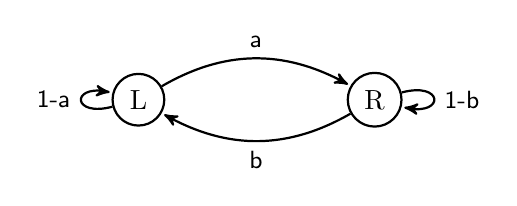
\begin{tikzpicture}[->,>=stealth',shorten >=1pt,auto,node distance=3cm,
                        thick,main node/.style={circle,draw}]
        \node[main node] (R) {R};
        \node[main node] (L) [left of=R] {L};
        \path[every node/.style={font=\sffamily\small}]
        (L) edge [loop left] node {1-a} (L)
            edge [bend left] node {a} (R)
        (R) edge [loop right] node {1-b} (R)
            edge [bend left] node {b} (L);
    \end{tikzpicture}
    \end{center}

    Then, the stationary distribution is 
    \begin{equation}
      \pi = \Big( \frac{b}{a+b}, \frac{a}{a+b} \Big)
    \end{equation}
    Notice that if $a = b = 0$, then this definition is ill-defined, and any probability distribution is invariant since $P = I_2$, the identity matrix. 
  \end{example}

  \begin{definition}[Recurrent]
    A state $x \in \mathcal{S}$ is \textit{recurrent} if
    \begin{equation}
      \mathbb{P}(X_n = n \text{ for some } n \geq 1 \, | \, X_0 = x\} = 1
    \end{equation}
    That is, if the initial state is $x$, the chain has probability $1$ of returning to $x$ at some later time. If a state is not recurrent, then the state is said to be \textit{transient}. That is, if $x$ is transient, there is some positive probability that the chain will never return to $x$. 
  \end{definition}

  \begin{definition}[Communication]
    Two states $x, y \in \mathcal{S}$ are said to \textit{communicate}, denoted $x \leftrightarrow y$, if there are positive integers $n$ and $m$ such that 
    \begin{equation}
      P^{(n)} (x, y) > 0 \text{ and } P^{(m)} (y, x) > 0
    \end{equation}
    That is, there is some positive probability that the chain can go from $x$ to $y$ and from $y$ to $x$ in some number of steps. 
  \end{definition}

  \begin{definition}[Irreducible Chains]
    If all pairs $x, y \in \mathcal{S}$ communicate, then the chain is said to be \textit{irreducible}. If there exists a pair of states that do not communicate, then the chain is said to be \textit{reducible}. 
  \end{definition}

  Note that the notion of communication is an equivalence relation between states. That is, it satisfies the properties. 
  \begin{enumerate}
    \item $x \leftrightarrow x$.
    \item $x \leftrightarrow y \implies y \leftrightarrow x$.
    \item $x \leftrightarrow y, y \leftrightarrow z \implies x \leftrightarrow z$.
  \end{enumerate}
  This relation partitions the state space $\mathcal{S}$ uniquely into transient states and irreducible sub-chains
  \begin{equation}
    \mathcal{S} = T \cup C_1 \cup C_2 \cup ...
  \end{equation}
  More specifically, $T$ is the set of all transient states, and the sets $C_k$ are \textit{closed communication classes}, meaning that
  \begin{enumerate}
    \item For all $x, y \in C_k$, $x \leftrightarrow y$. 
    \item $P(x, z) = 0$ whenever $x \in C_k$ but $z \not\in C_k$. 
  \end{enumerate}
  Note that for all $x, y \not\in T$, $x$ and $y$ communicate if and only if $x$ and $y$ are in the same class $C_k$. Moreover, once the chain reaches one of the sets $C_k$, it cannot leave $C_k$. 

  \begin{definition}[Period]
    For any state $x \in \mathcal{S}$, the \textit{period} of $x$ is defined to be
    \begin{equation}
      d(x) \equiv \gcd \{n \geq 1 \; | \; P^{(n)} (x, x) > 0\}
    \end{equation}
  \end{definition}

  \begin{theorem}
    It follows that if two states $x$ and $y$ communicate, then they must have the same period: $d(x) = d(y)$. It naturally follows that if the chain is irreducible, then all states must have the same period, and we can define the period of the chain to be $d(x)$ for any $x$ we choose.
  \end{theorem}

  \begin{definition}
    If an irreducible chain has period $1$, the chain is said to be \textit{aperiodic}. Otherwise, the chain is \textit{periodic} with period $d > 1$. 
  \end{definition}

  \begin{theorem}
    Suppose $|\mathcal{S}| < \infty$. If the chain is irreducible, then there always exists a unique stationary distribution $\pi$. If the chain is also aperiodic, then for any initial distribution $\nu$, 
    \begin{equation}
      \lim_{k \rightarrow \infty} \nu P^k = \pi
    \end{equation}
    Hence
    \begin{equation}
      \lim_{k \rightarrow \infty} P^{(k)}(x, y) = \pi(y)
    \end{equation}
    for all $x, y \in \mathcal{S}$. Furthermore, for any function $F: \mathcal{S} \longrightarrow \mathbb{R}$, the limit
    \begin{equation}
      \lim_{N \rightarrow \infty} \frac{1}{N} \sum_{n=1}^N F(X_n) = \sum_{x \in \mathcal{S}} F(x)\, \pi(x) = \mathbb{E} \big( F(x) \big)
    \end{equation}
    holds with probability $1$. In particular, the limit does not depend on the initial distribution. 
  \end{theorem}
  \begin{proof}
    The Frobenius Extension to Perron's theorem (Linear Algebra, Theorem 7.31) combined with its applications to stochastic matrices (Linear Algebra, Theorem 7.30) proves this statement. 
  \end{proof}

  \begin{definition}[First Visit]
    For each $x \in \mathcal{S}$, define the \textit{first visit} to $x$ by 
    \begin{equation}
      T_x \equiv \min\{ n \geq 1 \; | \; X_n = x\}
    \end{equation}
    This $T_x$ is an integer-valued random variable. We say $T_x = + \infty$ if $X_n$ never reaches $x$. Then, we define the \textit{mean return time} to $x$ by 
    \begin{equation}
      \mu_x \equiv \mathbb{E}\big( T_x \, | \, X_0 = x)
    \end{equation}
    If $x$ is transient, then $\mu_x = + \infty$, since there is positive probability that $T_x = + \infty$. 
  \end{definition}

  \begin{definition}
    It is possible that $x$ is recurrent while $\mu_x = +\infty$. If this is the case, then $x$ is said to be \textit{null-recurrent}. If $x$ is recurrent and $\mu_x < \infty$, then $x$ is said to be \textit{positive recurrent}. 
  \end{definition}

  \begin{theorem}
    An irreducible chain has a stationary probability distribution $\pi$ if and only if all states are positive recurrent. If a chain is irreducible and all states are positive recurrent, then 
    \begin{equation}
      \pi(x) = \frac{1}{\mu_x}
    \end{equation}
    for all $x \in \mathcal{S}$. $\pi$ is also unique. 
  \end{theorem}

  \subsubsection{Exit Probabilities}

    Suppose a chain is finite and irreducible. Let $a, b \in \mathcal{S}$ be given states, and let us define $h(x)$ to be the probability of hitting $b$ before $a$, given that we start from $x$. 
    \begin{equation}
      h(x) \equiv \mathbb{P} (X_n \text{ reaches } b \text{ before } a \, | \, X_0 = x)
    \end{equation}
    Clearly, $h(b) = 1$ and $h(a) = 0$. By conditioning on the first jump out of $x$, we also have 
    \begin{align*}
      h(x) & = \mathbb{P}(X_n \text{ reaches } b \text{ before } a \, | \, X_0 = x) \\
      & = \sum_{y} \mathbb{P}(X_n \text{ reaches } b \text{ before } a \, | \, X_1 = y, X_0 = x) \, \mathbb{P}(X_1 = y \,|\,X_0 = x) \\
      & = \sum_y \mathbb{P}(X_n \text{ reaches } b \text{ before } a \, | \,X_1 = y, X_0 = x) \, P(x, y) \\
      & = \sum_y \mathbb{P}(X_n \text{ reaches } b \text{ before } a \, | \,X_1 = y) \, P(x, y) \\
      & = \sum_y h(y) \, P(x, y) 
    \end{align*}
    The sum is over all $y \in \mathcal{S}$ for which $P(x, y) \neq 0$. This gives us a linear system of equations to solve for $h$
    \begin{align*}
      & h(x) = \sum_y P(x, y) h(y) \,\, \forall x \in \mathcal{S} \setminus \{a, b\}, \\
      & h(b) = 1, \\
      & h(a) = 0
    \end{align*}

  \subsubsection{Exit Prize}

    Let $B \subset \mathcal{S}$ be some subset of the state space, and let $g: B \longrightarrow \mathbb{R}$ be some function. Consider the function 
    \begin{equation}
      h(x) = \mathbb{E}\big( g(X_\tau) \, |\, X_0 = x \big)
    \end{equation}

    where $\tau = \min\{ n\geq 0 \,|\, X_n \in B\}$ is the first time that the chain reaches some state in the set $B$ (this time is random). We can interpret $g(y)$ as a "prize" that is awarded if the chain first reaches $B$ at state $y$, which means that $h(x)$ is the expected prize, given that $X_0 = x$. If $x \in B$, then $\tau = 0 \implies h(x) = g(x)$. But if $x \not\in B$, then by the same argument as shown in exit probabilities, it is true that $h$ satisfies the linear system of equations

    \begin{align*}
      & h(x) = \sum_g P(x, y)\,h(y), \;\; \forall x \in \mathcal{S} \setminus B, \\
      & h(x) = g(x), \;\; x \in B 
    \end{align*}

    Note that Exit probability system is a special case of the Exit prize system. In the former, we have defined $B = \{a, b\}$ and $g$ defined by $g(a) = 0, g(b) = 1$. 

  \subsubsection{Occupation Times, Absorbing States}

    Suppose that a chain on a finite $\mathcal{S}$ is irreducible. Let $B \subset \mathcal{S}$ be some subset of states and let $A = \mathcal{S} \setminus B$ be the other states. Then for $x \in A$, we wish to know how many steps the chain will take before reaching a state in the set $B$. We define 
    \begin{equation}
      \tau_B = \min\{n \geq 0 \,|\, X_n \in B\}
    \end{equation}
    which represents the first time that $X$ is in $B$, an integer valued random variable. We wish to compute
    \begin{equation}
      h(x) = \mathbb{E}(\tau_B \,|\, X_0 = x)
    \end{equation}
    Clearly, $h(y) = 0$ for all $y \in B$. For $x \in A$, it takes at least one step to reach $B \implies h(x) \geq 1$ for $x \in A$. We condition on the first step from $x$. This leads to the system 
    \begin{align*}
      h(x) = 1 + \sum_{y \in \mathcal{S}} P(x, y) \, \mathbb{E}(\tau_B \,|\, X_1 = y), & \forall x \in A = \mathcal{S} \setminus B
    \end{align*}
    Since the chain is time-homogeneous, this means that
    \begin{align*}
      h(x) = 1 + \sum_{y \in \mathcal{S}} P(x, y) \, h(y), & \forall x \in A 
    \end{align*}
    Since $h(y) = 0$ for all $y \in B$, we now have
    \begin{align*}
      h(x) = 1 + \sum_{y \in A} P(x, y) \, h(y), & \forall x \in A 
    \end{align*}
    To solve this system, let us define $M$ as the $|A| \times |A|$ submatrix of $P$ obtained by keeping only the entries $P(x, y)$ with $x, y \in A$. So, the system can be written as
    \begin{align*}
      h(x) = 1 + \sum_{y \in A} M(x, y) \, h(y), & \forall x \in A
    \end{align*}
    We can solve this system of equations through the equivalent matrix equation
    \begin{equation}
      (I - M) h = 1
    \end{equation}
    where $1 = (1, 1, ..., 1)^T$ is the column vector consisting of all $1$'s. The solution vector is therefore
    \begin{equation}
      h = (I - M)^{-1} 1
    \end{equation}
    So, for a particular $x \in A$, 
    \begin{equation}
      h(x) = \sum_{y \in A} (I - M)^{-1} (x, y)
    \end{equation}

    Alternatively, we can slightly modify the chain to chain $\Tilde{X}_n$ by replacing the transition probability matrix $P$ with another one defined as 
    \begin{equation}
      \Tilde{P}(x, y) = \begin{cases}
      P(x, y) & x \in A, y \in \mathcal{S} \\
      1 & x = y \in B \\
      0 & \text{else}
      \end{cases}
    \end{equation}

    This modification means that all transitions from state in $A$ to any other state are preserved and the only transitions from a state $x \in B$ are self loops. In particular, all transitions from states $x \in B$ to states $y \in A$ are removed. Therefore, under this modified transition matrix, the states in $B$ are absorbing states. The tail sum formula implies that
    \begin{equation}
      \mathbb{E}(\tau_B \,|\, X_0 = x) = \sum_{k=0}^\infty \mathbb{P}(\tau_B > k \,|\, X_0 = x)
    \end{equation}
    Notice that since the chain $X_n$ and $\Tilde{X}_n$ have the same transition rules before hitting a state $B$, we have 
    \begin{equation}
      P^{(k)} (x, y) = \Tilde{P}^{(k)} = M^{(k)}(x, y)
    \end{equation}
    where $M$ is the $|A| \times |A|$ submatrix defined previously. Therefore, putting this all together, we have
    \begin{align*}
      \mathbb{E}(\tau_B \,|\, X_0 = x) & = \sum_{k=0}^\infty \mathbb{P}(\tau_B > k \,|\, X_0 = x) \\
      & = \sum_{k=0}^\infty \mathbb{P}(\Tilde{X}_k \in A \,|\, X_0 = x) \\
      & = \sum_{k=0}^\infty \sum_{y \in A} \Tilde{P}^{(k)} (x, y) \\
      & = \sum_{k=0}^\infty \sum_{y \in A} M^{(k)} (x, y) \\
      & = \sum_{y \in A} \bigg( \sum_{k=0}^\infty M^{(k)} \bigg) (x, y) 
    \end{align*}
    Using a theorem from linear algebra, we can show that if all the eigenvalues of a $d \times d$ matrix $M$ have modulus strictly less than $1$, then $I-M$ is invertible and
    \begin{equation}
      \sum_{k=0}^\infty M^{(k)} = (I - M)^{-1}
    \end{equation}
    where $I$ is the $d \times d$ identity matrix. If $M$ is the $|A| \times |A|$ submatrix described above, one can show that $M$ has his property and that $I - M$ is invertible. Hence, 
    \begin{equation}
      \mathbb{E}(\tau_B \,|\, X_0 = x) = \sum_{y \in A} \bigg( \sum_{k=0}^\infty M^{(k)} \bigg) (x, y) = \sum_{y \in A} (I-M)^{-1} (x, y)
    \end{equation}
    which refers to the $(x, y)$ entry of the matrix $(I - M)^{-1}$. This is indeed consistent with our previous derivation of the formula for $h(x)$, the expected number of steps before the state reaches $B$. 

\subsection{Markov Chain Monte Carlo Algorithms}

  In statistics, Markov chain Monte Carlo (MCMC) methods comprise of a class of algorithms for sampling from a probability distribution by constructing a Markov chain that has the desired distribution as its equilibrium distribution. That way, by recording samples from the chain, one may get better approximations of the actual distribution. 

  Let there exist a state space $\mathcal{S}$ with some probability distribution $\pi(x)$ for every $x \in \mathcal{S}$. Clearly, 
  \begin{equation}
    \sum_{x \in \mathcal{S}} \pi(x) = 1
  \end{equation}
  but the problem is that we do not know that $\pi$ is. We do know, however, another function $f$ that is directly proportional to $\pi$. 
  \begin{equation}
    \pi(x) = \frac{f(x)}{c}, \text{ where } c = \sum_{x \in \mathcal{S}} f(x)
  \end{equation}
  is the normalizing constant. It is often the case that $c$ is unknown and the state space $\mathcal{S}$ is so large that computing $c$ directly is expensive. Therefore, we construct Markov chains that can provide approximations to $\pi$. 

  \subsubsection{Metropolis-Hastings Algorithm}

    This algorithm is useful because it does not require knowledge of the normalizing constant $c$. The algorithm only requires evaluations of 
    \begin{equation}
      \frac{\pi(x)}{\pi(y)} = \frac{f(x)}{f(y)}
    \end{equation}

    We first have the state space $\mathcal{S}$ consisting of all the possible states. We now construct (any) probability transition matrix $q$ for a Markov chain on $\mathcal{S}$. Note that $q$ is a $|\mathcal{S}| \times |\mathcal{S}|$ matrix and $q^T$ is a stochastic matrix. This matrix is constructed by the user and is completely well-defined and known. We start off with any initial state $x_0 \in \mathcal{S}$ and iterate the following 2-steps to construct a Markov chain. 

    \begin{enumerate}
      \item Given a state $X_n = x$, we generate a new state $X_{n+1}$ by first proposing a new state $y \in \mathcal{S}$ with probability $q(x, y)$ (determined from the matrix $q$). 
      \item With this chosen state $y$, we decide whether to accept to reject the proposal. With probability 
      \begin{equation}
        \min \bigg( 1, \frac{\pi(y) \,  q(y, x)}{\pi(x) \, q(x, y)} \bigg)
      \end{equation}
      we accept the proposal and set $X_{n+1} = y$. Otherwise, the proposal is rejected and the new state is the same $X_{n+1} = x$. 
    \end{enumerate}

    Note that there are two levels of randomness here: which state the new state $y$ will be and whether to accept this state to be the next one or not. If step two did not exist (i.e. the probability of accepting the proposal is always $1$), then this would just be a regular Markov chain represented by the matrix $q$. But the addition of step 2 means that while $q$ is used in constructing the discrete chain $X_n$, it is \textit{not} the transition probability matrix of $X_n$. 

    There is also a lot of flexibility on choosing $q$, although the performance of the algorithm (speed of convergence of the distribution of $X_n$ to the stationary distribution) will depend on the choice.

    \begin{proposition}
      For the chain defined by the Metropolis-Hastings algorithm, the distribution $\pi$ is stationary. 
    \end{proposition}
    \begin{proof}
      Let us write in shorthand 
      \begin{equation}
        \alpha(x, y) = \frac{\pi(y)\, q(y, x)}{\pi(x)\, q(x, y)}
      \end{equation}
      First, observe that if $x \neq y$, the transition probability for the chain defined by the algorithm is just
      \begin{equation}
        P(x, y) = q(x, y)\, \min\{1, \alpha(x, y)\}
      \end{equation}
      Next, we claim that for all $x, y \in \mathcal{S}$, 
      \begin{equation}
        \pi(x) P(x, y) = \pi(y) \, P(y, x)
      \end{equation}
      This condition is called \textit{detailed balance}. Assuming that $\alpha(x, y) \leq 1$, it is true that
      \begin{equation}
        \pi(x) P(x, y) = \pi(x) q(x, y) \frac{\pi(y) q(y, x)}{\pi(x) q(x, y)} = \pi(y) q(y, x)
      \end{equation}
      In this case, we also have $\alpha(y, x) = 1 / \alpha(x, y) \leq 1$. So, 
      \begin{equation}
        \pi(y) P(y, x) = \pi(y) q(y, x)
      \end{equation}
      and we have proved what we had claimed. Now, summing over $x$,
      \begin{equation}
        \sum_x \pi(x) P(x, y) = \sum_x \pi(y) P(y, x) = \pi(y) \sum_x P(y, x) = \pi(y)
      \end{equation}
      since $P^T$ is stochastic. 
    \end{proof}

  \subsubsection{Gibbs Sampling}

    Let $\mathcal{A} = \{a_1, ..., a_k\}$ be some finite set. Suppose that the state space 
    \begin{equation}
      \mathcal{S} = \mathcal{A} \times ... \times \mathcal{A} = \mathcal{A}^M
    \end{equation}
    for some $M \in \mathbb{N}$. The following algorithm generates a Markov chain on $\mathcal{S}$ with stationary distribution
    \begin{equation}
      \pi(x) = \frac{f(x_1, x_2, ..., x_M)}{c}, \;\; x = (x_1, x_2, ..., x_M) \in \mathcal{S} 
    \end{equation}
    where $c >0$ is a normalizing constant. Note that $|\mathcal{S}| = k^M$, so computing $c$ may be expensive when $M$ is large. The current state of the chain is denoted 
    \begin{equation}
      X_n = (X_n^1, X_n^2, ..., X_n^M)
    \end{equation}
    We think of $X_n$ as having $M$ components, each component taking values in $\mathcal{A}$. We start off with any initial state $X_0 = (X_0^1, X_0^2, ..., X_0^M)$ and construct a Markov chain by iterating the following two steps. 
    \begin{enumerate}
      \item Given $X_n = (X_n^1, X_n^2, ..., X_n^M)$, we generate the next state $X_{n+1}$ by picking a component index $i \in \{1, ..., M\}$ uniformly at random. 
      \item With this chosen, well-defined $i$, we choose a random $Y^i \in \mathcal{A}$ according to the distribution
      \begin{equation}
        \mathbb{P}(Y^i = a) = \frac{f\big(X_n^1 ,..., X_n^{i-1}, a, X_n^{i+1}, ..., X_n^M\big)}{\sum_{j=1}^k f\big(X_n^1 ,..., X_n^{i-1}, a_j, X_n^{i+1}, ..., X_n^M\big)}, \;\; a \in \{a_1, ..., a_k\}
      \end{equation}
      \item Then, set $X_{n+1} = \big(X_n^1, ..., X_n^{i-1}, Y^i, X_n^{i+1}, ..., X_n^M\big)$. 
    \end{enumerate}
    Note that at each step, only one component of $X_n$ is updated. Observe that the distribution above is also equal to 
    \begin{equation}
      \mathbb{P}(Y^i = a) = \frac{\pi\big(X_n^1 ,..., X_n^{i-1}, a, X_n^{i+1}, ..., X_n^M\big)}{\sum_{j=1}^k \pi \big(X_n^1 ,..., X_n^{i-1}, a_j, X_n^{i+1}, ..., X_n^M\big)}
    \end{equation}
    which is the marginal distribution of the $i$th component, given the values of the other components. 

    \begin{proposition}
      For the chain defined by this algorithm, the distribution $\pi$ is stationary. 
    \end{proposition}
    \begin{proof}
      We verify that the detailed balance condition holds. It is also helpful to note that $P(x, y) \neq 0$ if and only if $x$ and $y$ differ in one coordinate. 
    \end{proof}

\subsection{Continuous Time Markov Chains}

  As the name suggests, in a continuous time Markov chain $X_t$, the time parameter is continuous ($t \geq 0$). As before, the system jumps randomly between states in $\mathcal{S}$, but now the jumps may occur at any time and they occur randomly. This implies that there are \textit{two} sources of randomness:
  \begin{enumerate}
    \item \textit{where} the system jumps and 
    \item \textit{when} the system jumps
  \end{enumerate}

  \begin{definition}[Continuous Time Markov Chain]
    The Markov property in the continuous time case says that for any $s, t \geq 0$ and $y \in \mathcal{S}$, 
    \begin{equation}
      \mathbb{P}(X_{t + s} = y \, | \, X_t) = \mathbb{P}(X_{t+s} = y \, | \, X_r \; \forall 0 \leq r \leq t)
    \end{equation}
    Colloquially, the conditional distribution of $X_{t+s}$ given the history up to time $t$ is the same as the conditional distribution of $X_{t+s}$ given only $X_t$. Thus, if we know the current state at $t$, knowing information about the past doesn't help us better predict the future state $X_{t+s}$. 

    In order for the Markov property to hold, the times between jumps must be exponentially distributed random variables because it is the only density that has the memoryless property. This fact has already been stated in a theorem when covering Poisson arrival processes. This is what makes Exp$(\lambda)$ so important for continuous time Markov chains. 
  \end{definition}

  \begin{lemma}
    Let $T_1, T_2, ..., T_n$ be independent exponential random variables with rates $\lambda_1, \lambda_2, ..., \lambda_n$, respectively. Then the random variable $T \equiv \min\{T_1, T_2, ..., T_n\}$ is
    \begin{equation}
      T \sim \text{Exp}\Big(\sum_{i=1}^n T_i\Big)
    \end{equation}
    Moreover, 
    \begin{equation}
      \mathbb{P}(T_k = \min\{T_1, ..., T_n\}) = \frac{\lambda_k}{\lambda_1 + ... + \lambda_n}
    \end{equation}
  \end{lemma}

  We can interpret the lemma above by imagining that we have $n$ alarm clocks all set simultaneously, which will ring independently at random times. Suppose that clock $k$ will ring after $T_k$ units of time have expired, where $T_k$ is a random variable distributed as Exp$(\lambda_k)$. Then, $T = \min\{T_1, ..., T_n\}$ is the time at which the first ring occurs. 

  \begin{example}
    The simplest and the most important continuous time Markov chains is the Poisson arrival process. The process really has a single parameter $\lambda >0$ (the rate of process) by definition and is integer valued. At each jump time, the process increases by $1$, and the time between jumps are independent, distributed as Exp$(\lambda)$. 

    Notice that when $\lambda$ is large, the arrivals occur more frequently than when $\lambda$ is small, because the expected time between arrivals is $1/\lambda$. The second way we can interpret it is to choose an interval of time $t$ and let $X_t$ be the number of jumps that have occurred up to time $t$. It is a fact that $X_t$ is a integer-valued, Poisson$(\lambda t)$ distribution. That is, 
    \begin{equation}
      \mathbb{P}(X_t = k) = e^{-\lambda t} \frac{(\lambda t)^k}{k!}, \; k = 0, 1, 2, ...
    \end{equation}
    In particular, $\mathbb{E}(X_t) = \lambda t$ and $\Var(X_t) = \lambda t$. 
  \end{example}

\subsection{Branching Processes}

  \begin{definition}[Branching Process]
    A \textit{branching process} is a type of Markov chain modeling a population in which each individual produces a random number of children (possibly $0$) and dies. The state space is $\mathcal{S} = \{0, 1, 2, 3, ...\}$. Furthermore, there is a discrete-time version and a continuous time version of the chain. In the discrete case, the state is $Z_n$, the size of the population at time $n = 0, 1, 2, ...$, and in the continuous case, the state is $Z_t$ for $t \geq 0$. 
  \end{definition}

  \subsubsection{Discrete-time Branching Process}

    In the discrete case, all of the $Z_n$ individuals in the current generation branch at the same time and immediately die. The branching is independent and distributed according to the \textit{offspring distribution} $\{p_k\}_{k=0}^\infty$. Specifically, if $Z_n = m$, then 
    \begin{equation}
      Z_{n+1} = Y_1^n + Y_2^n + ... + Y_m^n
    \end{equation}
    where $Y_i^n$ represents the number of offspring the $i$th individual in the $n$th generation has. All of them are distributed as
    \begin{equation}
      \mathbb{P}(Y_i^n = k) = p_k, \; k = 0, 1, 2, 3, ...
    \end{equation}
    where $p_k$ is the probability that a parent has $k$ children. Note that if $p_0 \neq 0$, then there is positive probability that $Y_i^n = 0$ for all $i$, meaning that the population can go extinct. A sample branching process up to the second generation is shown below. 

    \begin{center}
    \begin{tikzpicture}[scale=0.8]
      \draw[fill] (0,4) circle (0.05);
      \draw[fill] (-2,2) circle (0.05);
      \draw[fill] (0,2) circle (0.05);
      \draw[fill] (2,2) circle (0.05);
      \draw[dashed] (0,4)--(-2,2);
      \draw[dashed] (0,4)--(0,2);
      \draw[dashed] (0,4)--(2,2);
      \draw[fill] (-3,0) circle (0.05);
      \draw[fill] (-1,0) circle (0.05);
      \draw[dashed] (-2,2)--(-3,0);
      \draw[dashed] (-2,2)--(-1,0);
      \draw[dashed] (2,2)--(3,0);
      \draw[dashed] (2,2)--(1,0);
      \draw[dashed] (2,2)--(2,0);
      \draw[fill] (3,0) circle (0.05);
      \draw[fill] (2,0) circle (0.05);
      \draw[fill] (1,0) circle (0.05);
      \node at (5,4) {$Z_0 = 1$};
      \node at (5,2) {$Z_1 = 3$};
      \node at (5,0) {$Z_2 = 5$};
      \draw[->] (4.3,4)--(3.5,4);
      \draw[->] (4.3,2)--(3.5,2);
      \draw[->] (4.3,0)--(3.5,0);
      \node at (-5, 3) {$Y_1^0 = 3$};
      \node at (-5, 1.5) {$Y_1^1 = 2$};
      \node at (-5, 1) {$Y_2^1 = 0$};
      \node at (-5, 0.5) {$Y_3^1 = 3$};
    \end{tikzpicture}
    \end{center}

    Suppose that the mean number of offspring of a single parent is finite. 
    \begin{equation}
      \mu = \mathbb{E}(Y) = \sum_{k=0}^\infty k \, \mathbb{P}(Y = k) = \sum_{k=0}^\infty k \, p_k < \infty
    \end{equation}
    If $Y_1$ and $Y_2$ are two independent, discrete random variables, we can define their convolution and use the fact that $\mathbb{P}(Y_i = k) = p_k$ to get
    \begin{align*}
      \mathbb{P}(Y_1 + Y_2 = k) & = \sum_j \mathbb{P}(Y_1 = k - j) \, \mathbb{P}(Y_2 = j) \\
      & = \sum_{j=0}^\infty p_{k-j} p_j, \;\; k = 0, 1, 2, ...
    \end{align*}
    This is a two-fold convolution of the sequence $\{p_k\}$ with itself, denoted
    \begin{equation}
      p_k^{*2} = \sum_{j=0}^\infty p_{k-j} \, p_j
    \end{equation}
    Extending this, we can find the $m$-fold convolution of the sequence $\{p_j\}$ with itself, represented by the sequence $\{p_j^{*m}\}$, where $p_k^{*m}$ is the $k$th term in this sequence. This gives us
    \begin{equation}
      p_k^{*n+1} = \sum_{j=0}^\infty p_{k-j} \, p_j^{*n}
    \end{equation}
    for all $n \in \mathbb{N}$. Using this, we can write down the transition probabilities for the Markov chain $Z_n$. 
    \begin{equation}
      \mathbb{P}(Z_{n+1} = k \, | \, Z_n = m) = \begin{cases}
      0 & \text{if } m = 0 \\
      p_k^{*m} & \text{if } m \geq 1, k \geq 0
      \end{cases}
    \end{equation}
    where $\mathbb{P}(Z_{n+1} = k \, | \, Z_n = m)$ represents the probability of the $n$th generation consisting of $m$ individuals producing a total of $k$ offspring for the $(n+1)$th generation. Thus, the branching process is completely determined by the distribution of $Z_0$ and the offspring distribution $\{p_k\}_{k=0}^\infty$. 

    \begin{lemma}
      Given this discrete-time branching process, let $\mu$ be the mean of the offspring distribution. Then, 
      \begin{equation}
        \mathbb{E}(Z_n \, | \, Z_0 = 1) = \mu^n
      \end{equation}
      If $\mu > 1$, the mean of $Z_n$ grows exponentially, and if $\mu_1$, the mean of $Z_n$ decreases exponentially. 
    \end{lemma}

  \subsubsection{Continuous-time Branching Process}

    A continuous time branching process $Z_t$ has very similar structure to the discrete time branching process, except that the times between branch events (for each individual) are independent exponentially distributed random variables Exp$(\lambda)$, where the parameter $\lambda> 0$ is the branching rate. It is as though each individual has an independent alarm clock which rings as a time that is Exp$(\lambda)$, independently of all other clocks. So, if there are currently $N$ individuals, then the next alarm will ring at rate $\lambda N$; that is, the time until the next ring is distributed as Exp$(\lambda N)$, since it is the minimum of $N$ independent Exp$(\lambda)$ random variables. When an individual branches (clock rings), that individual produces a random number of offspring, according to the offspring distribution $\{p_k\}$, as before. So, a continuous time branching process has the same geneological structure as the discrete time process, but the times between branch events is randomized. Consequently, whether or not the process eventually goes extinct, depends only on the offspring distribution, not on the branching rate $\lambda$. 

    Let $m_1(t) = \mathbb{E}(Z_t)$ denote the expected population size at time $t$. Then, it is a fact that $m_1(t)$ satisfies the ordinary differential equation
    \begin{equation}
      \frac{d}{d t} m_1 (t) = \lambda(\mu - 1) m_1 (t)
    \end{equation}
    where 
    \begin{equation}
      \mu = \sum_{k=1}^\infty k p_k
    \end{equation}
    is the mean of the offspring distribution. Solving this equation reveals that 
    \begin{equation}
      m_1 (t) = e^{\lambda (\mu-1) t} m_1 (0)
    \end{equation}
    If $\mu > 1$, the mean population size grows exponentially, and if $\mu < 1$, the mean population size decreases exponentially. 

  \subsubsection{Extinction Probability, Generating Functions}

    The expression for the transition probabilities of $Z_n$ (disrete case) is quite difficult to work with. Alternatively, it can be convenient to work with generating functions. 

    \begin{definition}[Generating Function]
      The \textit{generating function} for the offspring distribution is the function 
      \begin{equation}
        G(s) \equiv \sum_{k=0}^\infty p_k \, s^k = \mathbb{E}(s^Y)
      \end{equation}
      where $Y \sim \{p_k\}$ is a random variable representing the number of children produced by a given individual. Note that $G$ is a power series that simply encodes information about the offspring distribution (also a sequence) $\{p_k\}_{k=0}^\infty$. 
    \end{definition}

    \begin{theorem}[Properties]
      Properties of the generating function. 
      \begin{enumerate}
        \item The radius of convergence of $G(s)$ is at least $1$. $G(s)$ defines a continuous function on $|s| \leq 1$. 
        \item On the interval $[0,1]$, $G(s)$ is increasing and convex. If $p_0 + p_1 < 1$, then $G(s)$ is strictly convex for $s \in [0,1]$. 
        \item $G(0) = p_0$. 
        \item $G(1) = 1$. 
        \item $G^\prime(1^-) = \mu$ is the expected number of offspring of a single individual. 
      \end{enumerate}
    \end{theorem}
    \begin{proof}
      We use the fact that 
      \[\sum_{k=0}^\infty p_k = 1 \text{ and } 0 \geq p_k \geq \; \forall k = 0, 1, 2, ...\]
    \end{proof}

    \begin{theorem}
      Suppose that $Z_0 = 1$ and that $p_0 + p_1 < 1$. Then
      \begin{equation}
        \lim_{n \rightarrow \infty} \mathbb{P}(Z_n = 0) = \mathbb{P}(\text{eventual extinction}) = t
      \end{equation}
      where $t \in [0, 1]$ is the smallest non-negative root of the equation $t = G(t)$. If $\mu \leq 1$, then $t = 1$ (clearly, since the population will exponentially decrease on average). If $\mu > 1$, there is a positive probability that the population never goes extinct. 
    \end{theorem}
    \begin{proof}
      Let $t$ be the probability that an individual's descendent family tree goes extinct. That is, $t = \mathbb{P}(Z_n = 0$ for some $n \geq 1 \; | \; Z_0 = 1)$. To derive the equation $t = G(t)$, let us condition on the first generation, with $Y_1$ denoting the number of offspring of the single parent. 
      \begin{align*}
        t & = \mathbb{P}(\text{eventual extinction} \; | \; Z_0 = 1) \\
        & = \sum_{k=0}^\infty \mathbb{P}(\text{eventual extinction} \; | \; Z_0 = 1, Y_1 = k) \, \mathbb{P}(Y_1 = k \; | \; Z_0 = 1) \\
        & = \sum_{k=0}^\infty \mathbb{P}(\text{eventual extinction} \; | \;Z_0 =1, Y_1 = k) \, p_k
      \end{align*}
      That is, given that there are $k$ children of the first individual, the probability that this first individual's descendent family tree will go extinct is equal to the probability that each of the $k$ children's trees go extinct. These $k$ extinction events are independent. Therefore, 
      \begin{equation}
        \mathbb{P}(\text{eventual extinction} \; | \;Z_0 = 1, Y_1 = k) = t^k
      \end{equation}
      which implies that 
      \begin{equation}
        t = \sum_{k=0}^\infty \mathbb{P}(\text{eventual extinction} \; | \; Z_0 = 1, Y_1 = k) \, p_k = \sum_{k=0}^\infty t^k \, p_k = G(t)
      \end{equation}
      Additionally, under the hypothesis that $p_0 + p_1 < 1$, then $G(s)$ is strictly convex on $[0,1]$. Hence if $G^\prime (1) = \mu \leq 1$, the smallest non-negative root of $t = G(t)$ must be $t=1 \implies$ extinction occurs with probability 1. On the other hand, if $G^\prime (1) = \mu > 1$, then the smallest root of $t = G(t)$ occurs in the interval $[0,1)$. 
    \end{proof}

    Note that this result applies to both the discrete time case and the continuous time case. In continuous-time chains, whether or not the population goes extinct does not depend on $\lambda$, the rate at which individuals give birth. The $\lambda$ affects the time at which extinction occurs (if it occurs), but it does not affect the probability that it occurs. However, the extinction probability certainly does depend on the offspring distribution. 

    \begin{definition}[Counting Variable]
      A random variable $X$ is a \textit{counting variable} if it takes values in $\{0, 1, 2, ...\}$. 
    \end{definition}

    Note that generating functions is a mapping from $X$, the set of counting variables (all assumed to be pairwise independent) to the algebra of power series over variable $s$.
    \begin{equation}
      G: X \longrightarrow F[[s]]
    \end{equation}

    \begin{lemma}
      Let $X$ and $Y$ be two independent random counting variables, with generating functions $G_X (s) = \mathbb{E}(s^X)$ and $G_Y (s) = \mathbb{E}(s^Y)$. Then, the generating function for the random variable $Z = X + Y$ is $G_Z(s) = G_X (s) G_Y (s)$. That is, the generating function mapping $G$ is a homomorphism that maps addition to multiplication. In particular, if $X$ and $Y$ are iid, then $G_Z (s) = G_X (s)^2$. 
    \end{lemma}
    \begin{proof}
      Since $X$ and $Y$ are independent, 
      \begin{equation}
        G_Z (s) = \mathbb{E}(s^Z) = \mathbb{E}(s^{X+Y}) = \mathbb{E}(s^X s^Y) = \mathbb{E}(s^X) \mathbb{E}(s^Y) = G_X (s) G_Y (s)
      \end{equation}
    \end{proof}

    Applying this argument iteratively, we get the following lemma. 
    \begin{lemma}
      Let $N \geq 1$ be a fixed positive integer. Let $Y_1, Y_2, ..., Y_N$ be independent, identically distributed random counting variables with generating function $G_Y (s) = \mathbb{E}(s^Y)$. Then, the generating function for the sum $Z = Y_1 + ... + Y_n$ is 
      \begin{equation}
        G_Z (s) = G_Y (s)^N
      \end{equation}
    \end{lemma}

    Now, suppose that $N$ is not fixed, but another random variable. We wish to describe the distribution of the sum of a random number of random variables. 

    \begin{lemma}
      Let $Y_1, Y_2, Y_3, ...$ be a collection of independent, identically distributed random variables with generating function $G_Y (s) = \mathbb{E}(s^Y)$. Let $N$ be a random counting variable, independent of the $Y_i$. Let $N$ have generating function $G_N (s)$. Then the generating function for $Z = Y_1 + Y_2 + ... + Y_N$ is 
      \begin{equation}
        G_Z (s) = G_N \big( G_Y (s) \big)
      \end{equation}
    \end{lemma}
    \begin{proof}
      Just condition on $N = k$ 
      \begin{align*}
        G_Z (s) = \mathbb{E}(s^Z) & = \sum_{k=0}^\infty \mathbb{E}\big( s^Z \,|\, N=k\big) \, \mathbb{P}(N=k) \\
        & = \sum_{k=0}^\infty \mathbb{E}(s^{Y_1 + ... + Y_k} \,|\,N=k) \, \mathbb{P}(N=k) \\
        & = \sum_{k=0}^\infty G_Y (s)^k \, \mathbb{P}(N=k) \\
        & = \mathbb{E}\big( G_Y (s)^N \big) = G_N \big( G_Y (s) \big)
      \end{align*}
    \end{proof}

    \begin{theorem}
      Let $G(s)$ be the generating function for the offspring distribution $G(s) = \sum_{k=0}^\infty p_k s^k$. Suppose that $Z_0 = 1$ and let $G_n (s) = \mathbb{E}(s^{Z_n})$ be the generating function for the random variable $Z_n$. Then, 
      \begin{equation}
        G_{n+m} (s) = G_n \big(G_m (s)\big) = G_m \big( G_n (s) \big)
      \end{equation}
      Hence, 
      \begin{equation}
        G_n (s) = G(G(G(...(G(s))...))) \;\;\;\; \text{n-fold composition}
      \end{equation}
    \end{theorem}

    \begin{example}
      Suppose the offspring distribution is
      \begin{equation}
        p_k = q p^k, \;\; k \geq 0
      \end{equation}
      for some $p \in (0, 1)$, where $q = 1-p$. Thus, the number of children from a given parent is $Y = X - 1$, where $X \sim$ Geom$(q)$. Then, $\mathbb{E}(Y) = \frac{1}{q} - 1 = \frac{p}{q}$. With some computation, this means that
      \begin{equation}
        G(s) = \frac{q}{1- p s}
      \end{equation}
      and $t = \min \{1, \frac{q}{p}\}$. 
    \end{example}


\section{Common Distributions}

\subsection{Multivariate Gaussians}

Recall $X \sim \mathcal{N}(\mu, \sigma^2)$ implies that its PDF is 
\[f_X (x) = \frac{1}{\sigma \sqrt{2 \pi}} e^{-\frac{(x - \mu)^2}{2 \sigma^2}}\]
Now we will consider a Gaussian random \textit{vector}, which can be considered a vector of random variables  
\[\mathbf{X} = \begin{bmatrix} X_1 \\ X_2 \\ \vdots \\ X_n \end{bmatrix}\]
mapping from $\Omega$ to $\mathbb{R}^n$. It is not merely a vector where every $X_i$ is Gaussian, as we will show later. That is, a joint distribution that has all $n$ marginal distributions Gaussians does not make a multivariate Gaussian. 

This measurable function $\mathbf{X}: \Omega \rightarrow \mathbb{R}^n$ induces a probability law $\mathbb{P}_X$ on $\mathcal{B}(\mathbb{R}^n)$, and the Radon-Nikodym theorem states the existence of a PDF $f_X$ such that $\mathbb{P}_X (B) = \int_B f_X \,d\lambda$.

\subsubsection{Bivariate Gaussians}
Let us first begin with two-variable Gaussians. 

\begin{definition}[Standard Bivariate Gaussian RV]
A random variable $(X, Y)$ is said to be a \textbf{standard bivariate Gaussian} if its PDF is of form
\[f_{X, Y} (x, y) = \frac{1}{2 \pi \sqrt{1 - \rho^2}} \exp \bigg( -\frac{x^2 - 2 \rho x y + y^2}{2 (1 - \rho^2)} \bigg) \text{ for } \rho \in (-1, 1)\] 
\end{definition}

\begin{proposition}
Given a standard bivariate Gaussian $(X, Y)$, 
\begin{enumerate}
    \item $X$ and $Y$ are marginally distributed as $\mathcal{N}(0, 1)$. That is, if we integrate a variable (say, $x$) out, we will get a univariate standard Gaussian PDF of the other ($y$): 
    \[\int_{-\infty}^\infty \frac{1}{2 \pi \sqrt{1 - \rho^2}} \exp \bigg( -\frac{x^2 - 2 \rho x y + y^2}{2 (1 - \rho^2)}\bigg) \,dx = \frac{1}{\sqrt{2 \pi}} e^{-y^2 / 2}\]
    \item $\rho_{X, Y}$, the correlation coefficient of $X$ and $Y$, is equal to $\rho$. 
    \item The conditional distribution of $X$ given $Y = y$ is $X \mid Y = y \sim \mathcal{N} (\rho y, 1 - \rho^2)$. That is, 
    \[f_{X \mid Y} (x \mid y) = \frac{1}{2 \pi \sqrt{1 - \rho^2}} \exp \bigg( -\frac{x^2 - 2 \rho x y + y^2}{2 (1 - \rho^2)}\bigg) = \frac{1}{ \sqrt{2 \pi (1 - \rho^2)}} \, \exp\bigg( - \frac{(x - (\rho y))^2}{2 (1 - \rho^2)} \bigg)\]
    \item From (3), we can see that the conditional expectation $\mathbb{E}[X \mid Y = y] = \rho y$ since $X \mid Y = y$ has mean at $\rho y$. Therefore, the conditional expectation of $X$ given $Y$ (which is a random variable) is 
    \[\mathbb{E}[X \mid Y] = \rho Y\]
    i.e. $\mathbb{E}[X \mid Y]$ is a linear function of $Y$. 
\end{enumerate}
\end{proposition}

The formula of the general bivariate Gaussian $\mathbf{X} = (X_1, X_2)$ PDF is messy, but we will put it here. 
\[f_{X_1, X_2} (x, y) = \frac{\sigma_1 \sigma_2 \sqrt{1 - \rho^2}} \exp \bigg[ -\frac{1}{2} \bigg( \frac{(x_1 - \mu_1)^2}{\sigma_1^2} + \frac{(x_2 - \mu_2)^2}{\sigma_2^2} - 2 \rho \frac{(x_1 - \mu_1)}{\sigma_1} \frac{(x_2 - \mu_2)}{\sigma_2}\bigg)\bigg]\]
It is cleaner to put it into matrix form. 
\[f_{X_1, X_2} (x_1 , x_2) = \frac{1}{2 \pi \sqrt{\mathrm{det}(\boldsymbol{\Sigma})}} \exp \bigg( - \frac{(\mathbf{x} - \boldsymbol{\mu})^T \boldsymbol{\Sigma}^{-1} (\mathbf{x} - \boldsymbol{\mu})}{2} \bigg) \]
where 
\[\mathbf{x} = \begin{pmatrix} x_1 \\ x_2 \end{pmatrix}, \;\; \boldsymbol{\mu} = \begin{pmatrix} \mu_1 \\ mu_2 \end{pmatrix} , \;\; \boldsymbol{\Sigma} = \mathbb{E}\big[ (\mathbf{X} - \boldsymbol{\mu}) (\mathbf{X} - \boldsymbol{\mu})^T \big] = \begin{pmatrix} \mathrm{Var}(X_1) & \mathrm{Cov}(X_1, X_2) \\
\mathrm{Cov}(X_1, X_2) & \mathrm{Var}(X_2) \end{pmatrix}\]

Note that visually, $\boldsymbol{\Sigma}$ will determine how much the Gaussian distribution is "stretched" on one way or another. Obviously, the "peak" of the distribution will be $\boldsymbol{\mu}$. If $\boldsymbol{\Sigma} = I$, then we could visualize the Gaussian distribution as being perfectly symmetric. However, if we scale the distribution up to a certain constant (below shown $\boldsymbol{\Sigma} = I$, $\boldsymbol{\Sigma} = 0.61 I$, $\boldsymbol{\Sigma} = 2 I$), we get
\begin{center}
    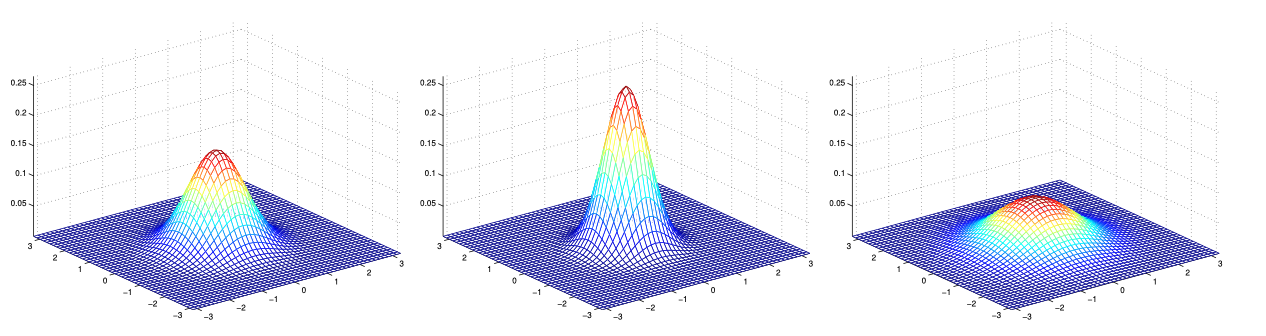
\includegraphics[scale=0.65]{img/Gaussian_Distribution.png}
\end{center}

Now we've made a remark before that given a multivariate distribution $\mathbf{X} = (X_1, \ldots, X_n)$, all of its marginal distributions being Gaussian does not mean that $\mathbf{X}$ is a multivariate Gaussian. We give a counterexample. 

\begin{example}
Let $Y_1, Y_2$ be iid random variables distributed according to the PDF 
\[f_Y (y) = \sqrt{\frac{2}{\pi}} e^{-y^2 / 2} \text{ for } y > 0\]
which we can interpret as a one-sided Gaussian. Let $W \sim \mathrm{Bernoulli}(\frac{1}{2})$ be independent of $Y_1$ and $Y_2$. Now, define the random variables 
\[X_1 = W \, Y_1 \text{ and } X_2 = W \, Y_2\]
This is clearly not a multivariate Gaussian, even though the marginals are $X_1, X_2 \sim \mathcal{N}(0, 1)$. We could make the degenerate case that $X_1 = X_2$, which would make the image of $(X_1, X_2)$ just the line at $x_1 = x_2$, but we can think of this as a degenerate Gaussian with a singular $\boldsymbol{\Sigma}$. 

\begin{figure}[H]
  \centering 
  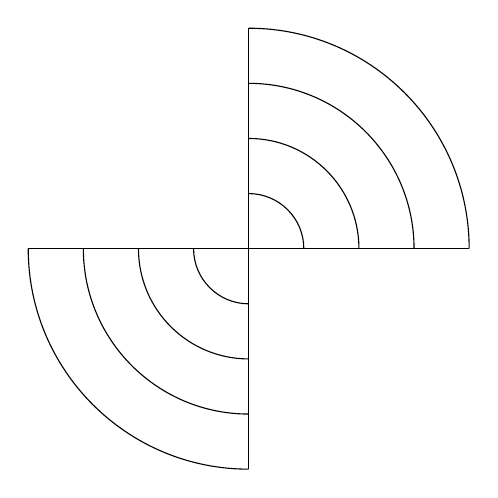
\begin{tikzpicture}[scale=0.7]
    % Draw the x and y axes
    \draw (-4,0) -- (4,0);
    \draw (0,-4) -- (0,4);
    
    \draw (1,0) arc (0:90:1);
    \draw (-1,0) arc (180:270:1);
    \draw (2,0) arc (0:90:2);
    \draw (-2,0) arc (180:270:2);
    \draw (3,0) arc (0:90:3);
    \draw (-3,0) arc (180:270:3);
    \draw (4,0) arc (0:90:4);
    \draw (-4,0) arc (180:270:4);
  \end{tikzpicture}
  \caption{Now note that $Y_1$ and $Y_2$ are both positive, and since $X_1$ and $X_2$ are both dependent on the same value of $W$, it is either $X_1$ and $X_2$ are both positive or both negative. So, the joint distribution of $X_1, X_2$ will be on only the 1st and 3rd quadrant with no mass on the 2nd and 4th. }
  \label{fig:not_multi_gaussian}
\end{figure}
\end{example}

\subsubsection{Multivariate Gaussians}

There are three equivalent definitions of multivariate Gaussians of $n$-variables. 

\begin{definition}[Multivariate Gaussian]
Let us have a vector-valued random variable $\mathbf{X} = (X_1 \ldots X_n)^T \sim \mathcal{N}(\boldsymbol{\mu}, \boldsymbol{\Sigma})$. 
\begin{enumerate}
    \item $\mathbf{X}$ is a \textbf{multivariate Gaussian distribution} with mean $\boldsymbol{\mu} \in \mathbb{R}^n$ and symmetric, positive-definite covariance matrix $\boldsymbol{\Sigma} \in \mathbb{R}^{n \times n}$ if its probability density function is
    \[f_X (x) = \frac{1}{(2\pi)^{n/2} \mathrm{det}(\boldsymbol{\Sigma})^{1/2}} \exp\bigg( -\frac{1}{2} (x-\boldsymbol{\mu})^T \boldsymbol{\Sigma}^{-1} (x - \boldsymbol{\mu})\bigg)\]
    The covariance matrix $\boldsymbol{\Sigma}$ is the $n \times n$ matrix whose $(i, j)$th entry is $\Cov(X_i, X_j)$. That is, for any random vector $\mathbf{X}$ with mean $\boldsymbol{\mu}$, its covariance matrix 
    \[\boldsymbol{\Sigma} = \mathbb{E}\big[ (\mathbf{X} - \boldsymbol{\mu}) (\mathbf{X} - \boldsymbol{\mu})^T \big] = \mathbb{E}[\mathbf{X} \mathbf{X}^T] - \boldsymbol{\mu} \boldsymbol{\mu}^T\]
    is positive definite and symmetric, which implies by the spectral theorem we can break it down into $n$ orthogonal eigenspaces of positive eigenvalues. 

    \item $X$ is a multivariate Gaussian distribution if it can be expressed as 
    \[\mathbf{X} = \mathbf{D} \mathbf{w} + \boldsymbol{\mu}\]
    where $\mathbf{w}$ is a vector of independent $\mathcal{N}(0, 1)$ Gaussians, $\boldsymbol{\mu} \in \mathbb{R}^n$, and $\mathbf{D} \in \mathbb{R}^{n \times n}$. The mean of $\mathbf{X}$ is $\boldsymbol{\mu}$ and its covariance is $\boldsymbol{\Sigma} = \mathbf{D} \mathbf{D}^T$; $\mathbf{D}$ is called the \textbf{standard deviation matrix}. When modeling high-dimensional Gaussians, this way is most computationally feasible. 

    \item $X$ is a multivariate Gaussian distribution if for every $\mathbf{a} \in \mathbb{R}^n$, $\mathbf{a}^T \mathbf{x}$ is a Gaussian RV. This means that if we take $\mathbf{a} = \mathbf{0}$, then the entire $\mathbf{X}$ is constantly $0$, which we will take to be the degenerate Gaussian with mean, variance $0$. 
\end{enumerate}
The $n$ semi-axes of the $(n-1)$-dimensional isocontour ellipsoid formed by an $n$-dimensional Gaussian distribution are precisely the normalized eigenvectors of $\boldsymbol{\Sigma}$ multiplied by their eigenvalues. 
\end{definition}


If we let $\boldsymbol{\Sigma} = \mathbf{I}$, then this means that all the $X_i$'s are pairwise uncorrelated since $\Sigma_{ij} = \Cov (X_i, X_j) = 0$. In general, this does not mean that the $X_i$'s are independent, but for joint Gaussians, this also implies independence! 

\begin{theorem}
Given multivariate Gaussian $\mathbf{X} = (X_1 \ldots X_n)^T \sim \mathcal{N}(\boldsymbol{\mu}, \boldsymbol{\Sigma})$, the $X_i$'s are pairwise independent if and only if they are uncorrelated. 
\end{theorem}
\begin{proof}
We can expand the PDF of $\mathbf{X}$ as 
\begin{align*}
    f_X (x) & = \frac{1}{(2 \pi)^{n/2}} \exp \bigg( -\frac{1}{2} (x - \mu)^T (x - \mu) \bigg) \\
    & = \bigg(\frac{1}{\sqrt{2\pi}} \bigg)^n \exp \bigg( \sum_{i=1}^n -\frac{1}{2} (x_i - \mu_i)^2 \bigg) \\
    & = \prod_{i=1}^n \frac{1}{\sqrt{2\pi}} \exp \bigg( -\frac{1}{2} (x_i - \mu_i)^2 \bigg)
\end{align*}
which is the product of $n$ single-variable Gaussians $X_i$. Therefore this means that independence and uncorrelation are equivalent! 
\end{proof}

Therefore, if the nondiagonal entries of the covariance matrix are all $0$, then we know that the variables are all uncorrelated and therefore independent. 



\end{document}
